\section{การวิเคราะห์ระบบ}

\subsection{แผนภาพ use case ของระบบ}

แผนภาพ use case ของระบบโดยรวมแสดงในภาพที่ \ref{fig:ch4_9} โดยแบ่งออกเป็น 3 ระบบย่อย ได้แก่ ระบบจัดการบัญชีผู้ใช้ ระบบใช้งานหนังสือ และระบบจัดการผู้ดูแล 

\begin{figure}[H]
\centering
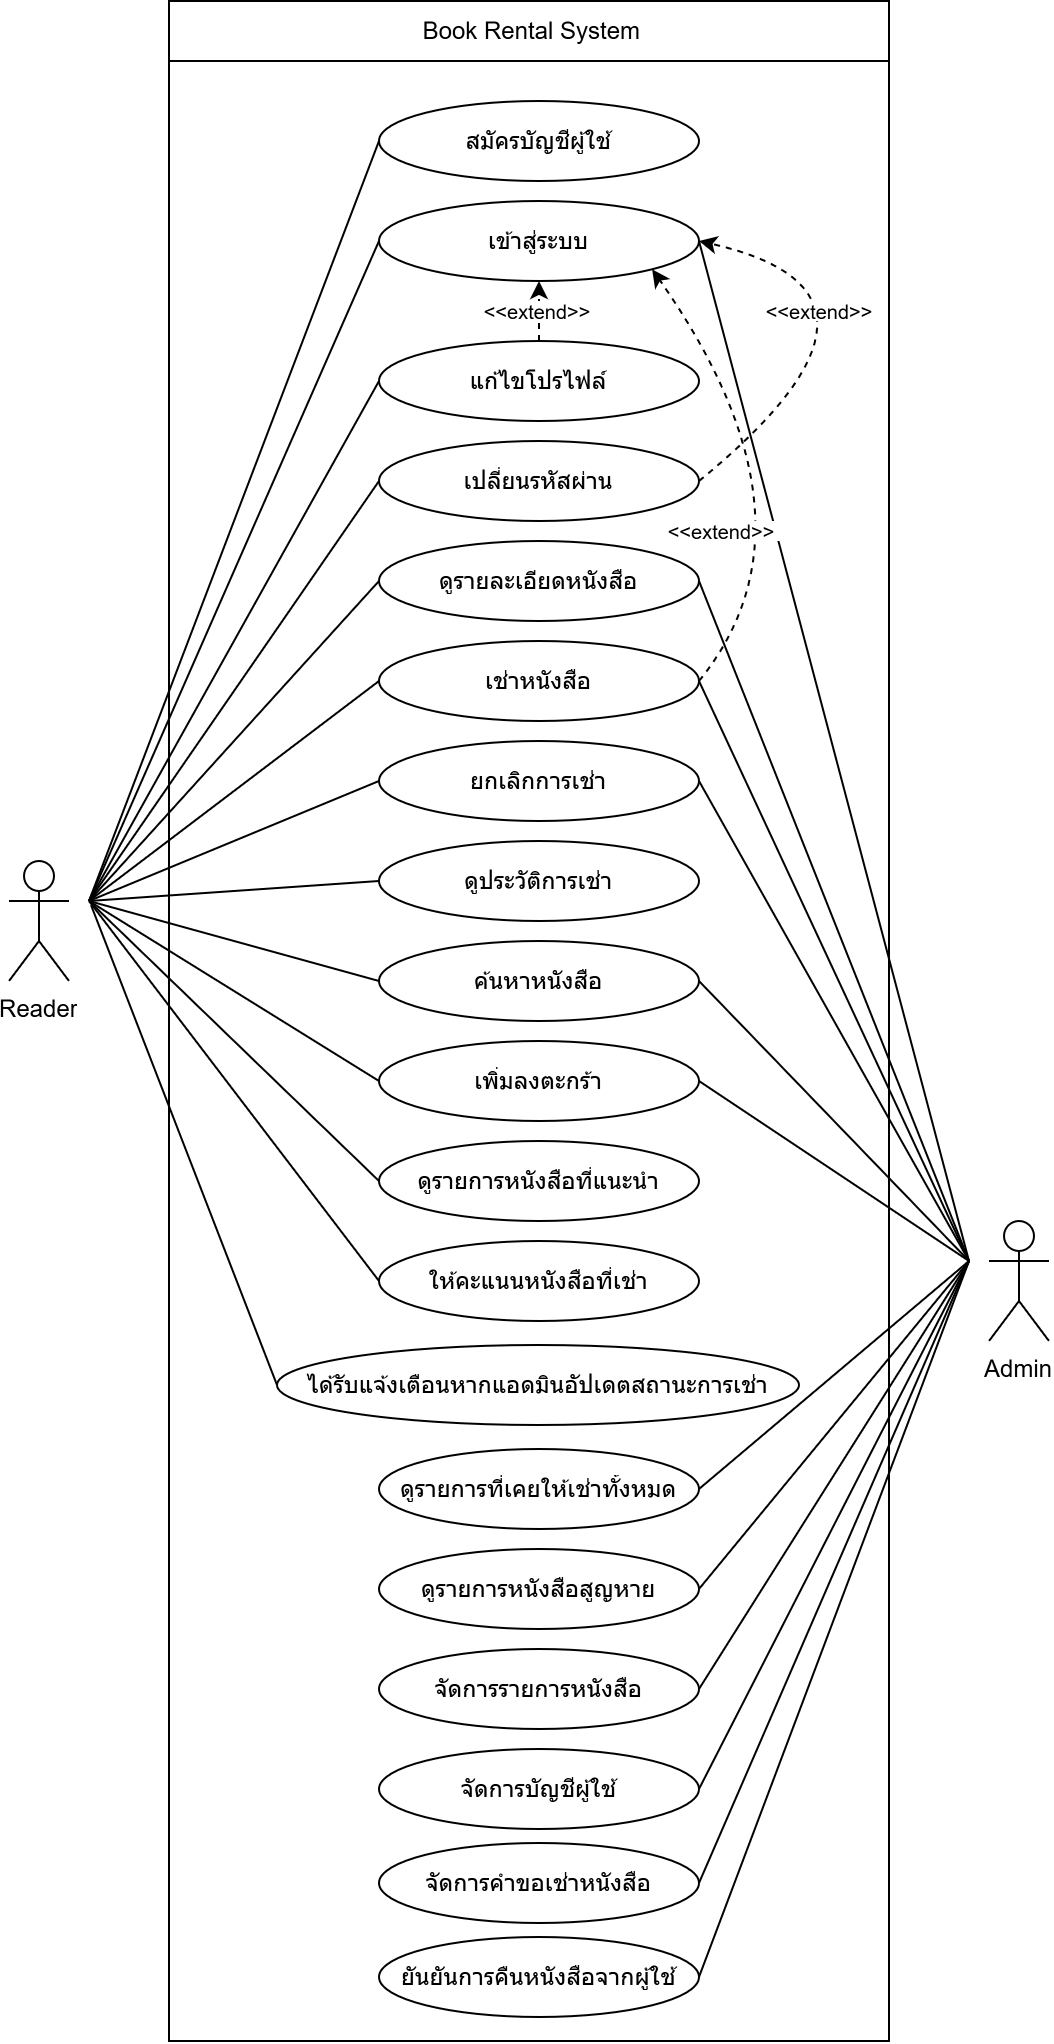
\includegraphics[width=0.5\textwidth]{images/4image9.png}
\caption{Overall Use Case Diagram}
\label{fig:ch4_9}
\end{figure}

ภาพที่ \ref{fig:ch4_9} แสดงแผนภาพ Use Case ภาพรวมของระบบเช่าหนังสือการ์ตูน ประกอบด้วยผู้ใช้งานหลัก 2 กลุ่ม คือ ผู้ใช้ทั่วไป และผู้ดูแลระบบ ซึ่งมีการเชื่อมโยงกับฟังก์ชันการทำงานต่างๆ ของระบบ โดยแบ่งเป็นกลุ่มงานหลักได้แก่ การจัดการบัญชี การค้นหาและเช่าหนังสือ การจัดการคำสั่งเช่า และการบริหารจัดการข้อมูลโดยผู้ดูแลระบบ

\bigskip
\begin{figure}[H]
\centering
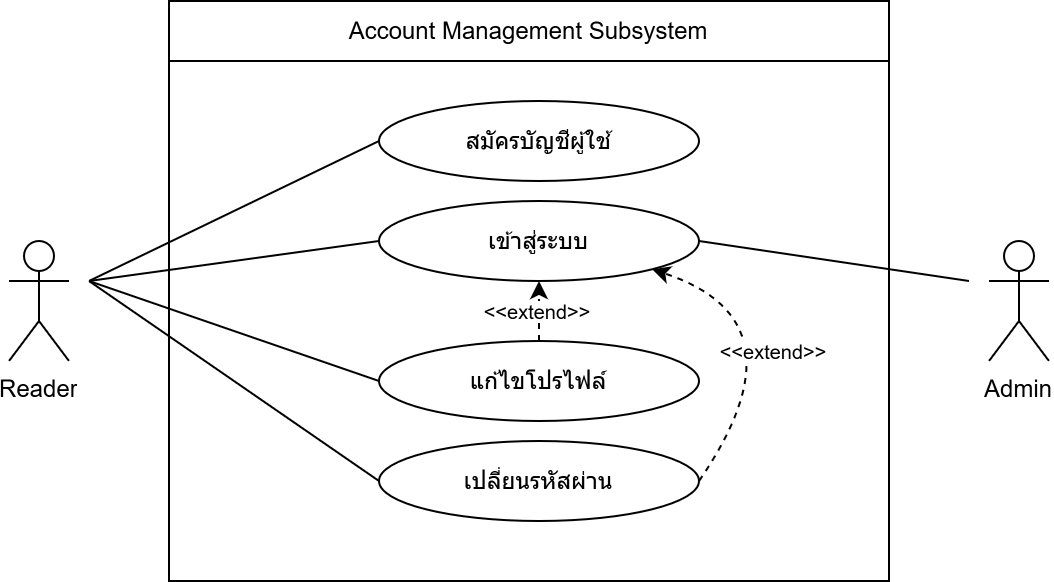
\includegraphics[width=0.9\textwidth]{images/4image11.png}
\caption{Account Management Subsystem}
\label{fig:ch4_11}
\end{figure}

ภาพที่ \ref{fig:ch4_11} แสดงระบบย่อยการจัดการบัญชีผู้ใช้ ซึ่งครอบคลุมฟังก์ชันการสมัครสมาชิก การเข้าสู่ระบบ การแก้ไขโปรไฟล์ส่วนตัว และการออกจากระบบ โดยผู้ใช้ทั่วไปสามารถดำเนินการเหล่านี้ได้ด้วยตนเอง เพื่อบริหารจัดการบัญชีและข้อมูลส่วนบุคคลของตนเองภายในระบบ

\begin{figure}[H]
\centering
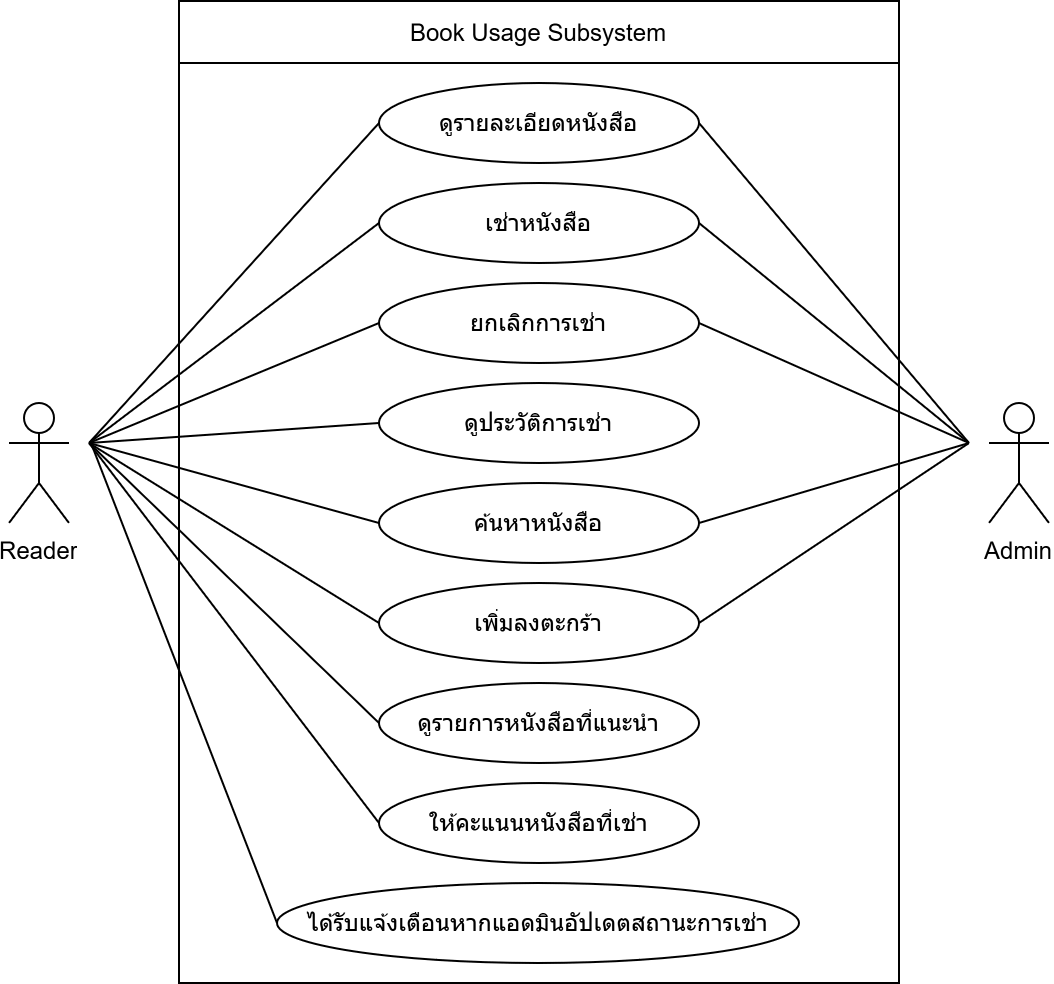
\includegraphics[width=0.9\textwidth]{images/4image13.png}
\caption{Book Usage Subsystem}
\label{fig:ch4_13}
\end{figure}

ภาพที่ \ref{fig:ch4_13} แสดงระบบย่อยการใช้งานหนังสือการ์ตูน ประกอบด้วยฟังก์ชันหลักที่ผู้ใช้สามารถทำได้ ได้แก่ การค้นหาและเรียกดูหนังสือการ์ตูน การดูรายละเอียดและตัวอย่างเนื้อหา การเพิ่มหนังสือลงในตะกร้า การดูประวัติการเช่า การยกเลิกคำสั่งเช่า และการให้คะแนนหรือรีวิวหนังสือที่เคยเช่า ซึ่งฟังก์ชันเหล่านี้เป็นกระบวนการหลักของระบบเช่าหนังสือการ์ตูนออนไลน์

\begin{figure}[H]
\centering
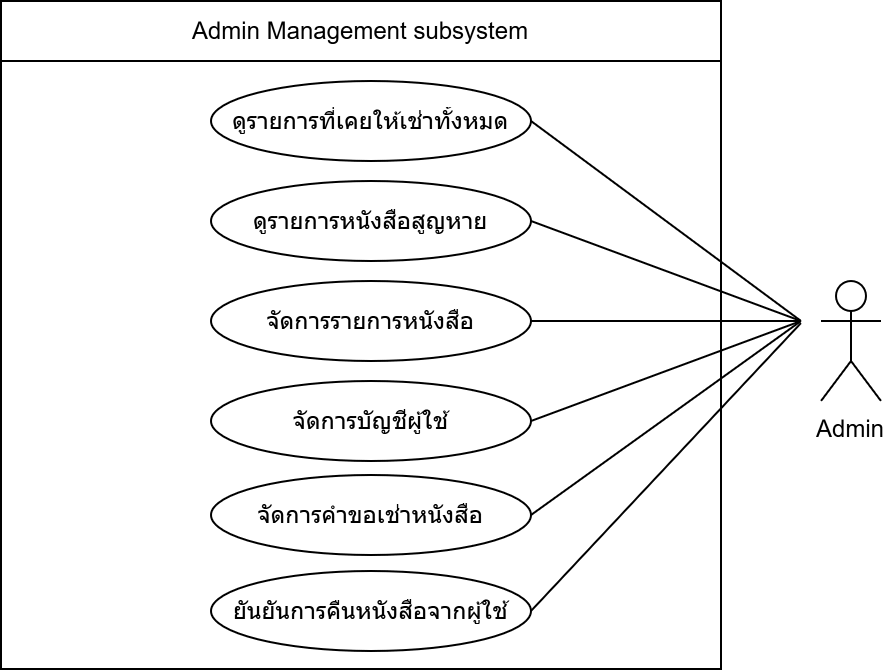
\includegraphics[width=0.9\textwidth]{images/4image15.png}
\caption{Admin Management subsystem}
\label{fig:ch4_15}
\end{figure}

ภาพที่ \ref{fig:ch4_15} แสดงระบบย่อยการจัดการผู้ดูแลระบบ ซึ่งประกอบด้วยฟังก์ชันสำหรับผู้ดูแลระบบในการบริหารจัดการทรัพยากรและข้อมูลต่างๆ ได้แก่ การจัดการข้อมูลหนังสือการ์ตูน (เพิ่ม แก้ไข ลบ) การจัดการข้อมูลผู้ใช้ การอนุมัติหรือปฏิเสธคำสั่งเช่า การตรวจสอบการคืนหนังสือและเรียกเก็บค่าปรับกรณีชำรุดหรือส่งคืนล่าช้า ตลอดจนการดูประวัติธุรกรรมทั้งหมดในระบบ เพื่อให้สามารถควบคุมและดูแลการดำเนินงานของระบบได้อย่างมีประสิทธิภาพ

\subsection{แผนภาพ sequence diagram ของระบบ}

แผนภาพ sequence diagram อธิบายลำดับการทำงานของระบบในแต่ละฟังก์ชัน โดยแบ่งการแสดงผลออกเป็นส่วนๆ ตามลำดับการทำงาน ได้แก่ การสมัครสมาชิก (ภาพที่ \ref{fig:ch4_66}) การค้นหาหนังสือและตะกร้าสินค้า (ภาพที่ \ref{fig:ch4_67}--\ref{fig:ch4_70}) การส่งคำขอเช่า (ภาพที่ \ref{fig:ch4_71}--\ref{fig:ch4_74}) ประวัติการเช่า (ภาพที่ \ref{fig:ch4_75}--\ref{fig:ch4_78}) การให้คะแนน (ภาพที่ \ref{fig:ch4_79}--\ref{fig:ch4_82}) การจัดการคำสั่งเช่าของผู้ดูแลระบบ (ภาพที่ \ref{fig:ch4_83}--\ref{fig:ch4_87}) การจัดการหนังสือของผู้ดูแลระบบ (ภาพที่ \ref{fig:ch4_88}--\ref{fig:ch4_93}) และการจัดการผู้ใช้ของผู้ดูแลระบบ (ภาพที่ \ref{fig:ch4_94}--\ref{fig:ch4_100})

\begin{figure}[H]
\centering
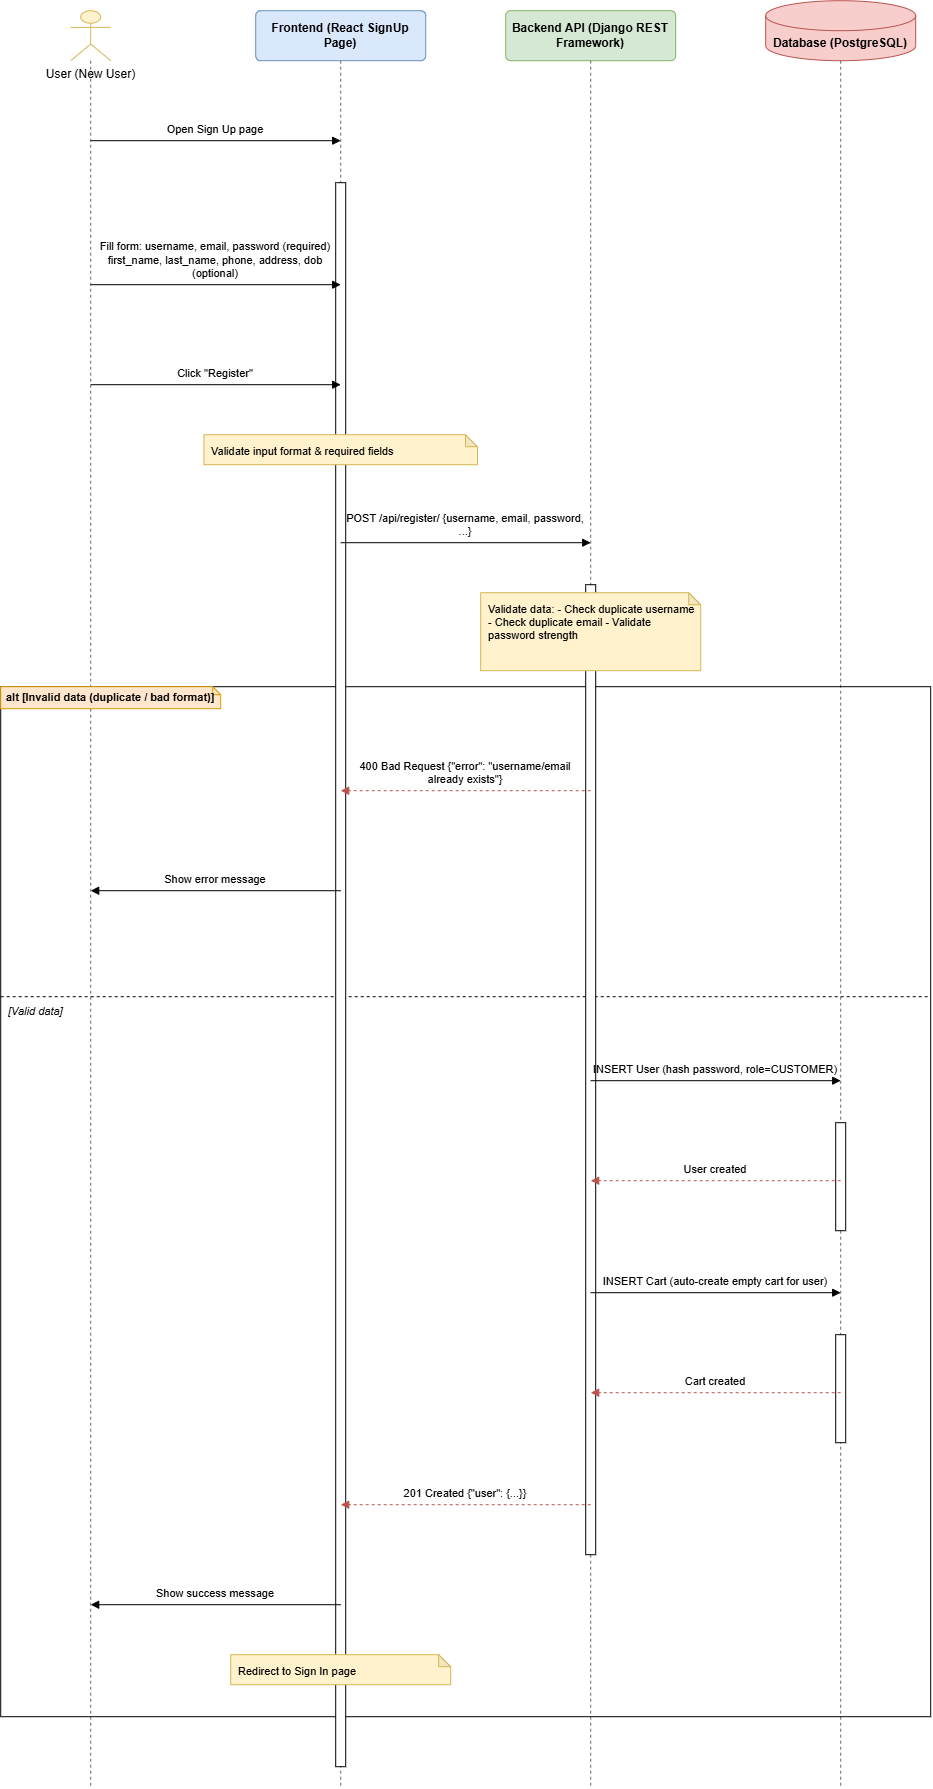
\includegraphics[width=0.8\textwidth]{images/4image66.png}
\caption{Register Sequence Diagram - Manga Rental System}
\label{fig:ch4_66}
\end{figure}

ภาพที่ \ref{fig:ch4_66} แสดง Sequence Diagram ของกระบวนการสมัครสมาชิก เริ่มต้นจากผู้ใช้กรอกข้อมูลส่วนตัวผ่าน Frontend ระบบจะส่งข้อมูลไปยัง Backend API เพื่อตรวจสอบความถูกต้องและซ้ำซ้อนของข้อมูล หากผ่านการตรวจสอบ ระบบจะบันทึกข้อมูลผู้ใช้ใหม่ลงในฐานข้อมูลและส่งผลลัพธ์การสมัครสมาชิกสำเร็จกลับไปยังผู้ใช้

\bigskip
\begin{figure}[H]
\centering
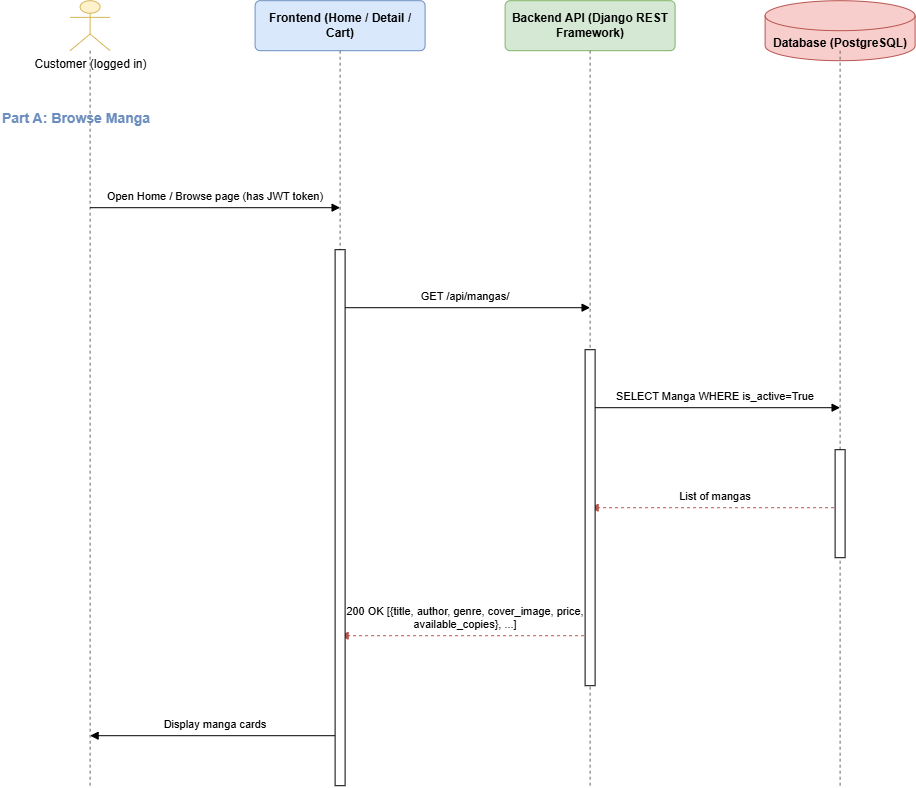
\includegraphics[width=0.85\textwidth]{images/4image67.png}
\caption{Browse and Cart Sequence Diagram - Part A: Browse Manga}
\label{fig:ch4_67}
\end{figure}

\begin{figure}[H]
\centering
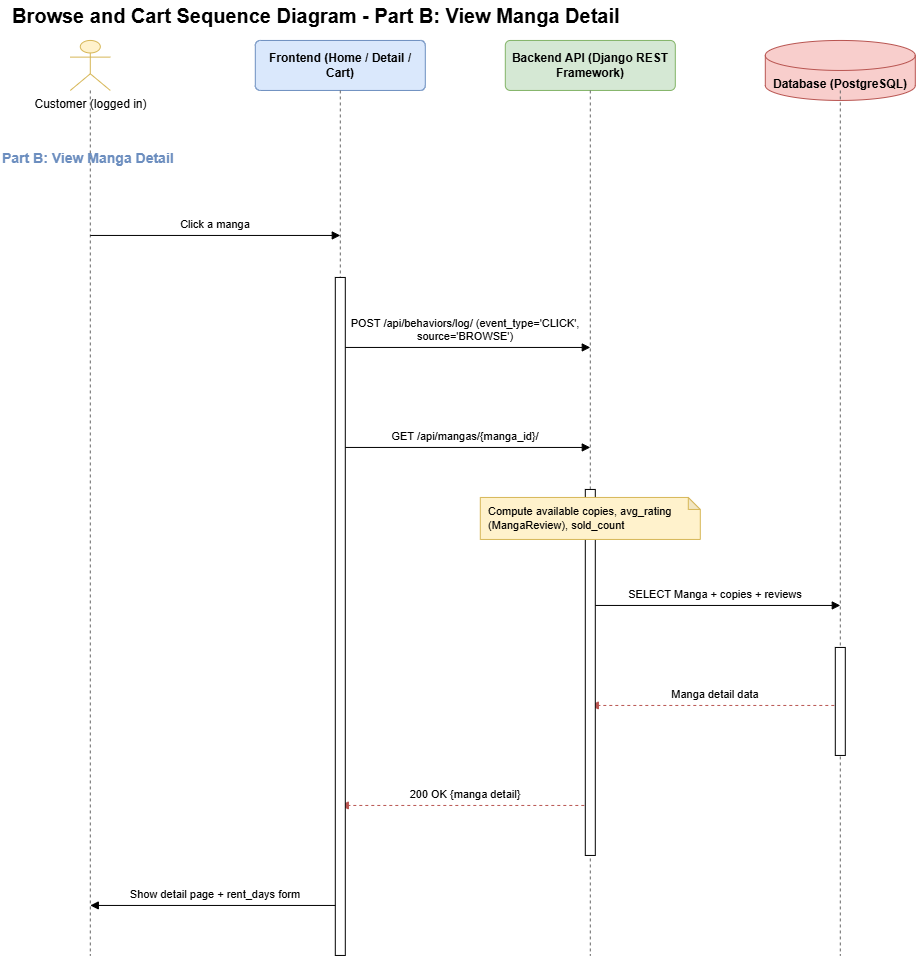
\includegraphics[width=0.85\textwidth]{images/4image68.png}
\caption{Browse and Cart Sequence Diagram - Part B: View Manga Detail}
\label{fig:ch4_68}
\end{figure}

\begin{figure}[H]
\centering
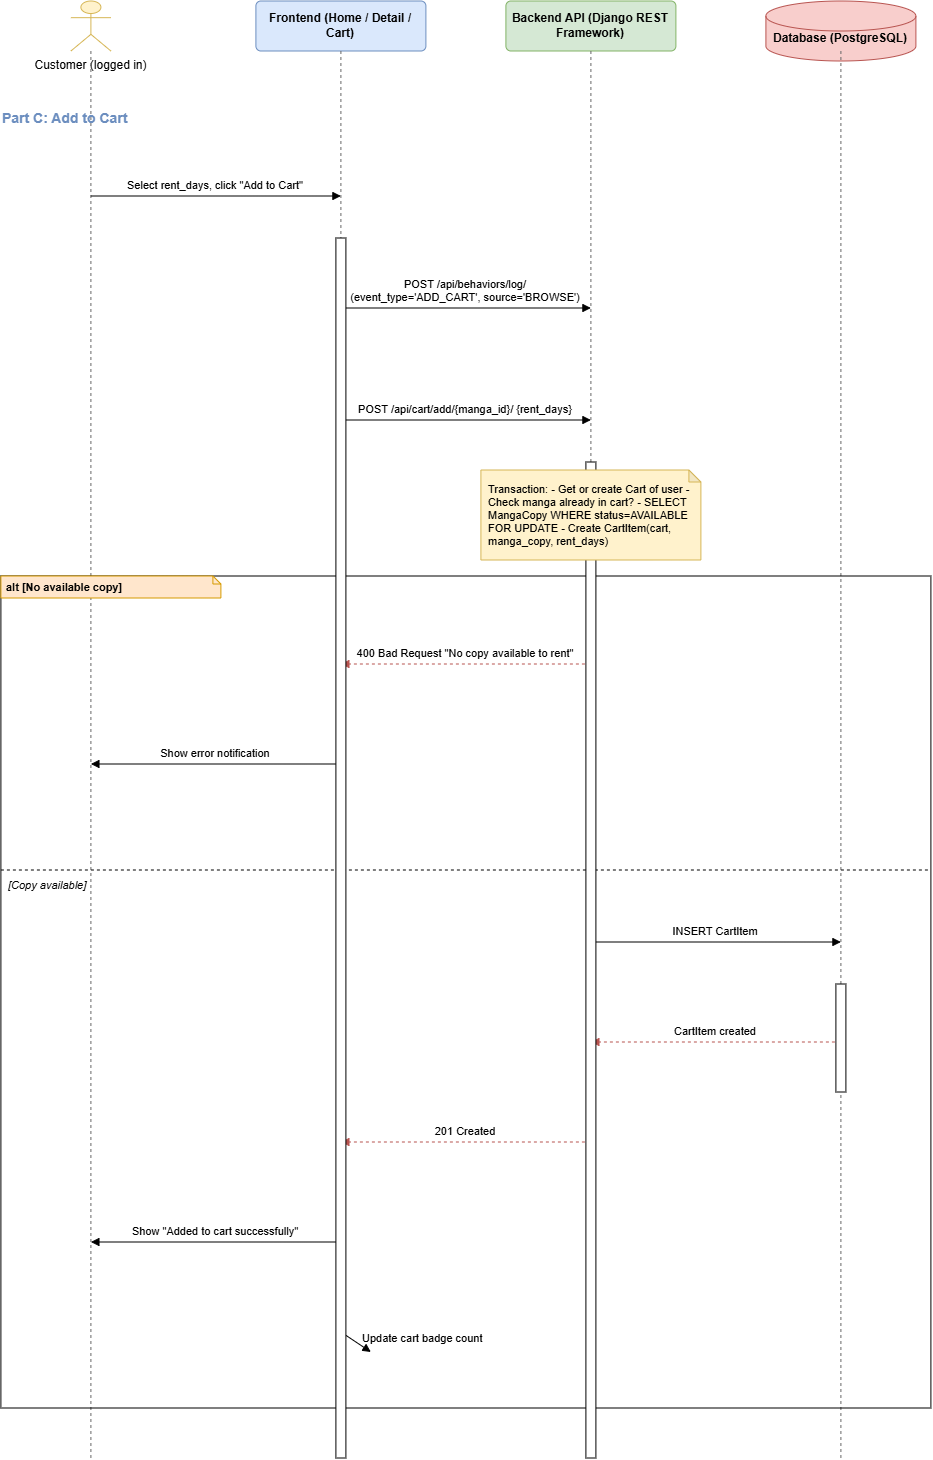
\includegraphics[width=0.85\textwidth]{images/4image69.png}
\caption{Browse and Cart Sequence Diagram - Part C: Add to Cart}
\label{fig:ch4_69}
\end{figure}

\begin{figure}[H]
\centering
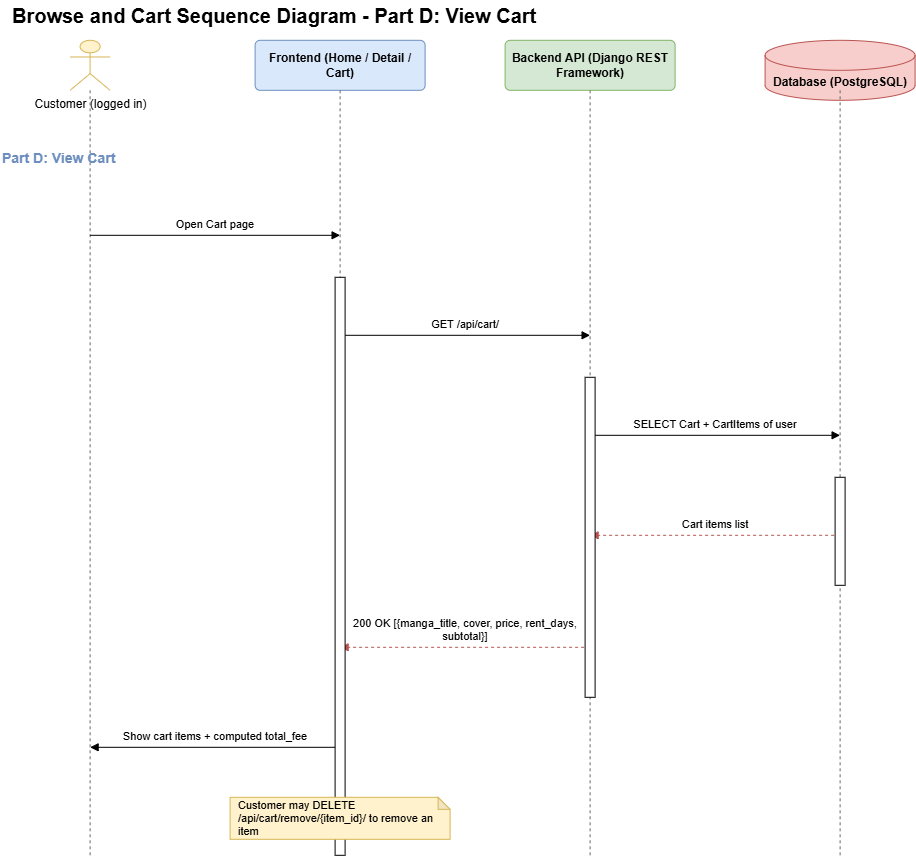
\includegraphics[width=0.85\textwidth]{images/4image70.png}
\caption{Browse and Cart Sequence Diagram - Part D: View Cart}
\label{fig:ch4_70}
\end{figure}

ภาพที่ \ref{fig:ch4_67}--\ref{fig:ch4_70} แสดง Sequence Diagram ของกระบวนการค้นหาหนังสือและจัดการตะกร้าสินค้า โดยครอบคลุม 4 ฟังก์ชันหลัก ได้แก่ การเรียกดูรายการหนังสือที่มีในระบบพร้อมกับข้อมูลคำแนะนำ (\ref{fig:ch4_67}) การดูรายละเอียดและตัวอย่างเนื้อหาของหนังสือที่สนใจ (\ref{fig:ch4_68}) การเพิ่มหนังสือเข้าตะกร้า (\ref{fig:ch4_69}) และการแสดงรายการสินค้าในตะกร้าพร้อมคำนวณราคารวม (\ref{fig:ch4_70}) ซึ่งแต่ละขั้นตอนมีการส่งผ่านข้อมูลระหว่าง Frontend, Backend API และ Database

\begin{figure}[H]
\centering
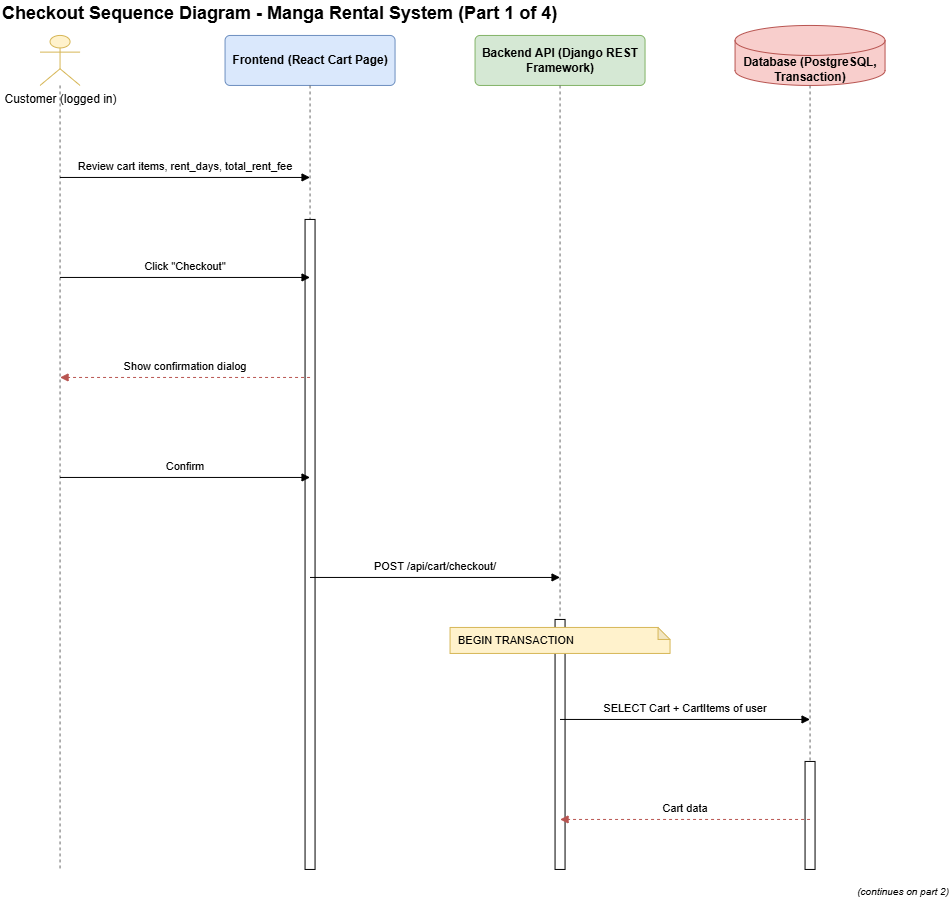
\includegraphics[width=0.85\textwidth]{images/4image71.png}
\caption{Checkout Sequence Diagram - Manga Rental System (Part 1 of 4)}
\label{fig:ch4_71}
\end{figure}

\begin{figure}[H]
\centering
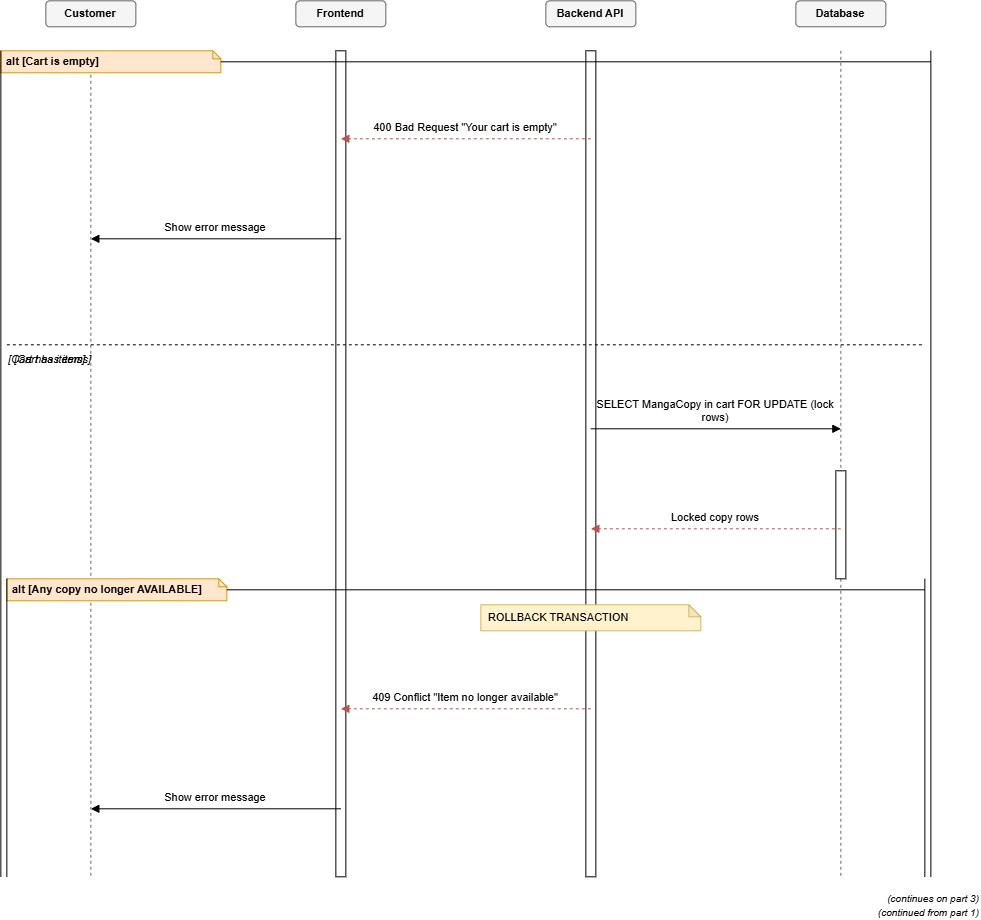
\includegraphics[width=0.85\textwidth]{images/4image72.png}
\caption{Checkout Sequence Diagram - Manga Rental System (Part 2 of 4)}
\label{fig:ch4_72}
\end{figure}

\begin{figure}[H]
\centering
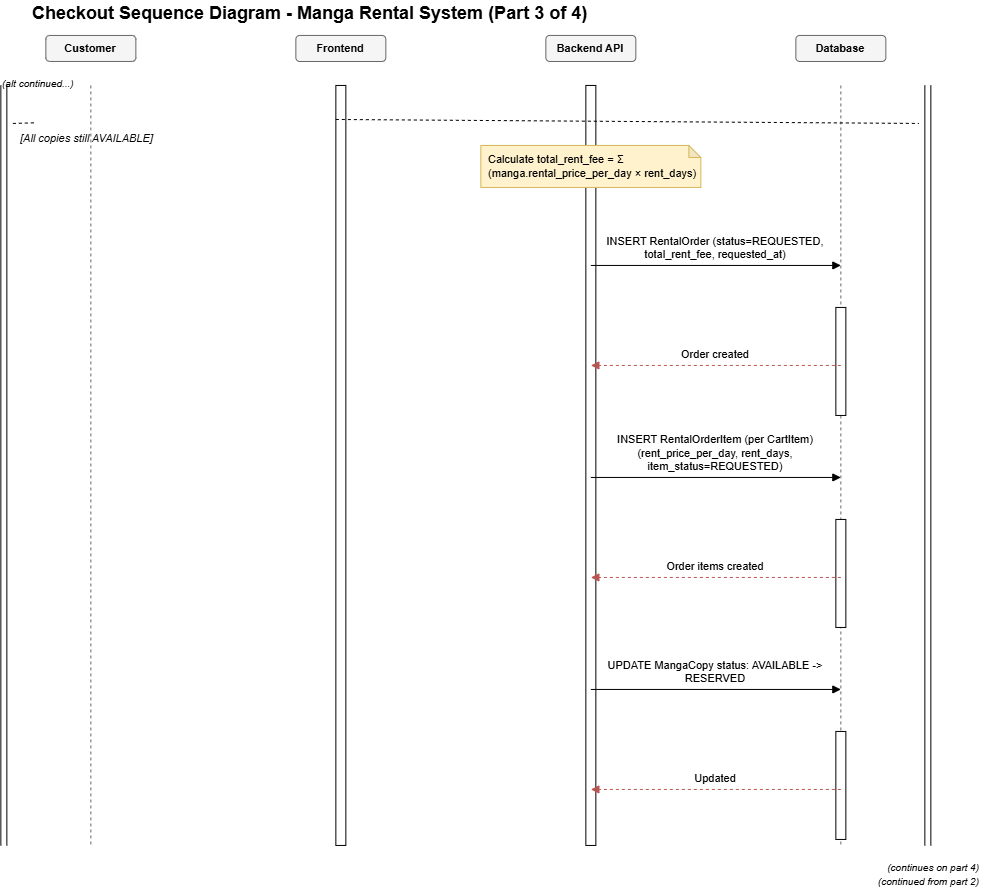
\includegraphics[width=0.85\textwidth]{images/4image73.png}
\caption{Checkout Sequence Diagram - Manga Rental System (Part 3 of 4)}
\label{fig:ch4_73}
\end{figure}

\begin{figure}[H]
\centering
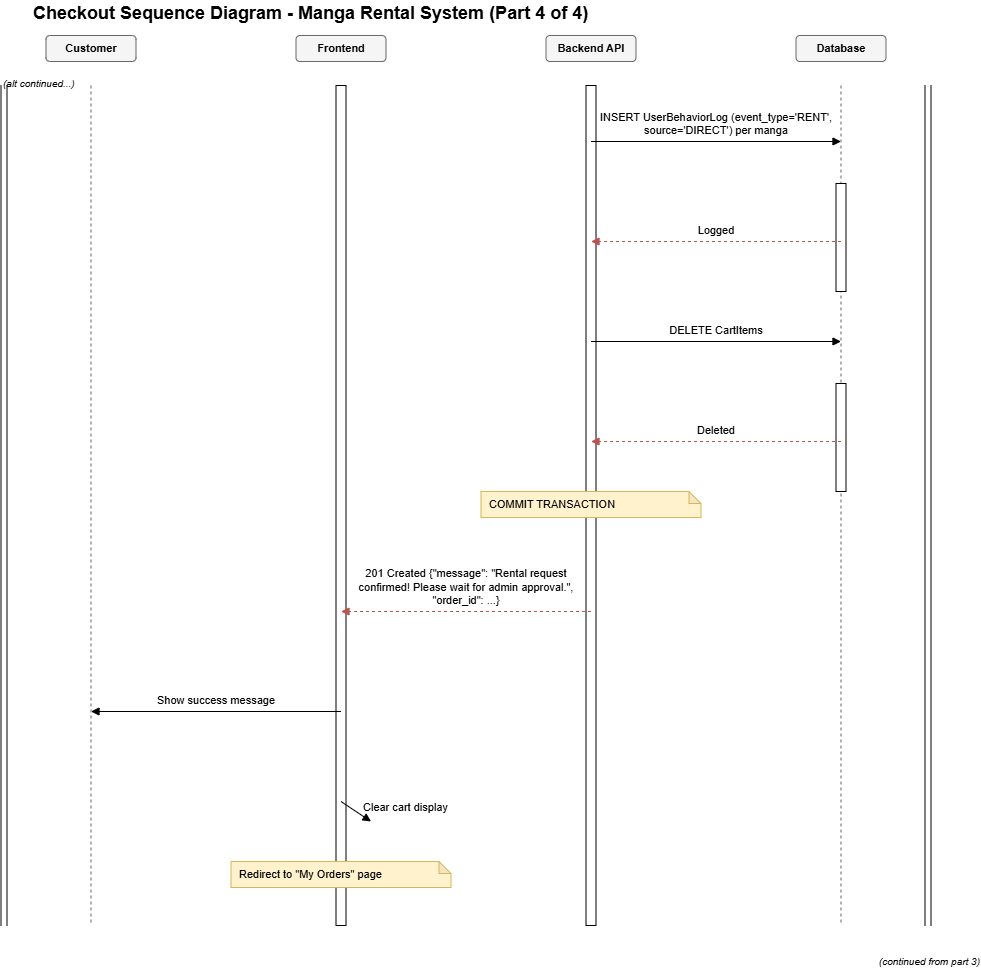
\includegraphics[width=0.85\textwidth]{images/4image74.png}
\caption{Checkout Sequence Diagram - Manga Rental System (Part 4 of 4)}
\label{fig:ch4_74}
\end{figure}

ภาพที่ \ref{fig:ch4_71}--\ref{fig:ch4_74} แสดง Sequence Diagram ของกระบวนการส่งคำขอเช่า โดยเริ่มจากผู้ใช้กดยืนยันการการเช่า ระบบจะดึงข้อมูลตะกร้าสินค้าและตรวจสอบสถานะความพร้อมของหนังสือแต่ละเล่ม จากนั้นจะสร้างคำสั่งเช่า และรายการคำสั่ง บันทึกลงในฐานข้อมูล อัปเดตสถานะหนังสือเป็น "ไม่ว่าง" และล้างตะกร้าสินค้า สุดท้ายจะส่งข้อมูลการเช่าสำเร็จพร้อมรายละเอียดคำสั่งเช่ากลับไปยังผู้ใช้

\begin{figure}[H]
\centering
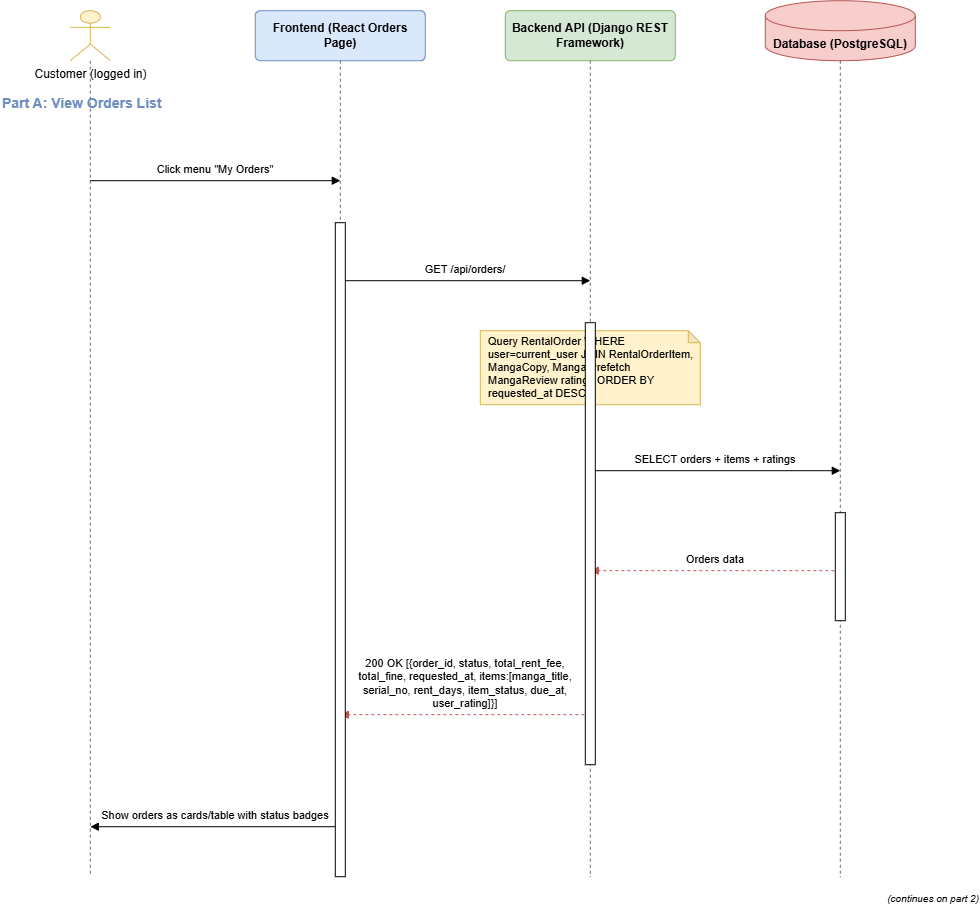
\includegraphics[width=0.85\textwidth]{images/4image75.png}
\caption{My Order Sequence Diagram - Manga Rental System (Part 1 of 4 - View Orders List)}
\label{fig:ch4_75}
\end{figure}

\begin{figure}[H]
\centering
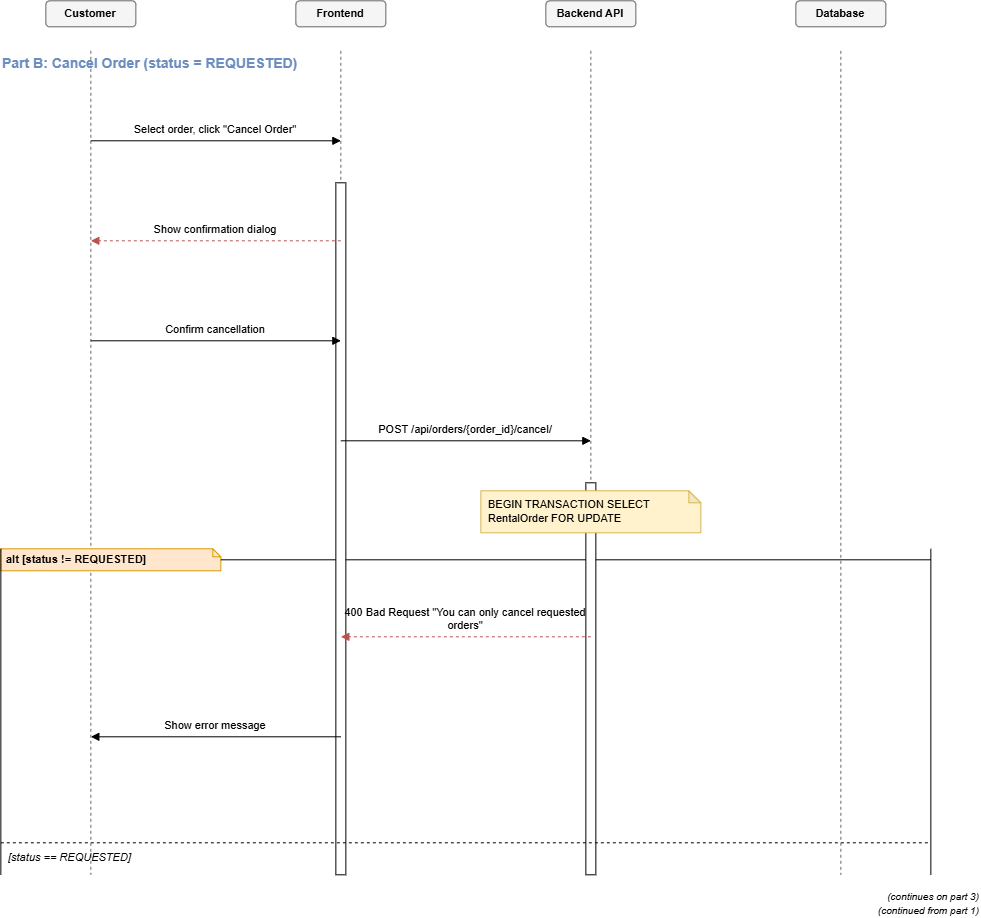
\includegraphics[width=0.85\textwidth]{images/4image76.png}
\caption{My Order Sequence Diagram - Manga Rental System (Part 2 of 4 - Cancel Order (1/2))}
\label{fig:ch4_76}
\end{figure}

\begin{figure}[H]
\centering
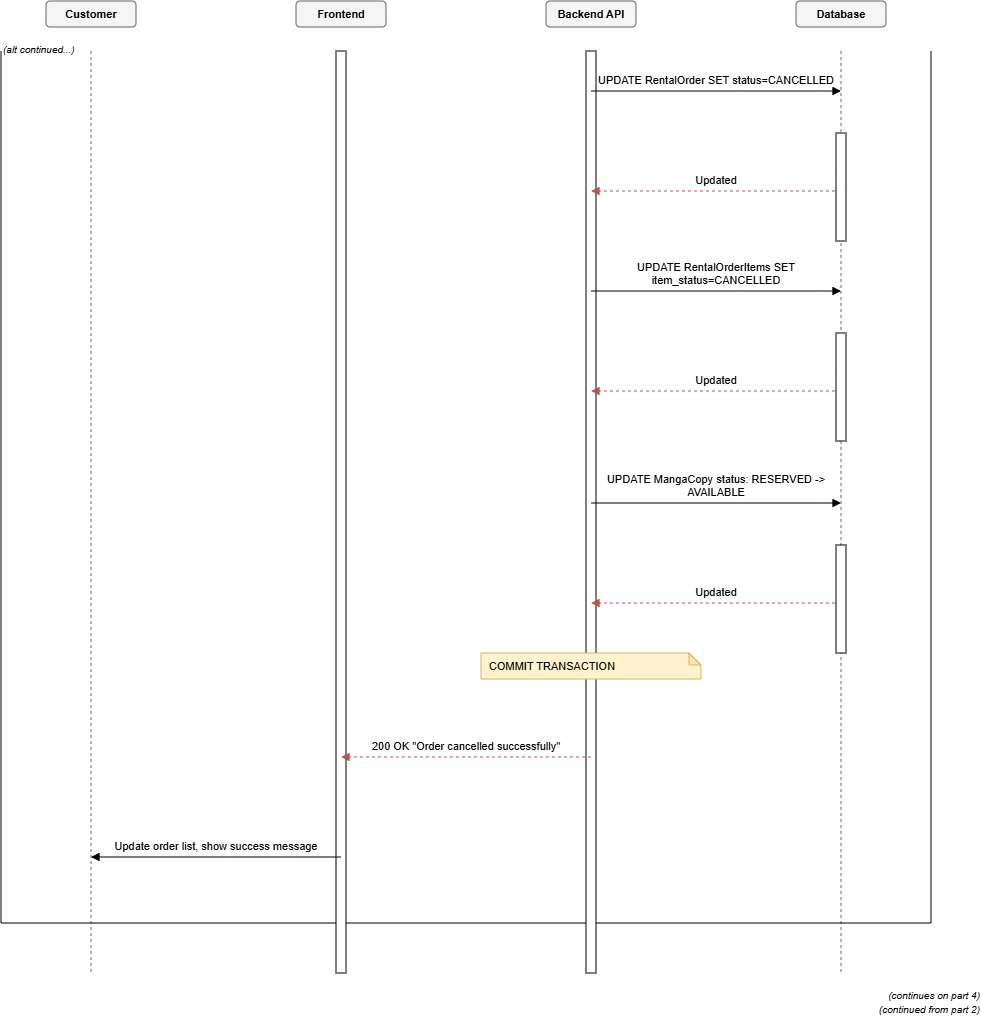
\includegraphics[width=0.85\textwidth]{images/4image77.png}
\caption{My Order Sequence Diagram - Manga Rental System (Part 3 of 4 - Cancel Order (2/2))}
\label{fig:ch4_77}
\end{figure}

\begin{figure}[H]
\centering
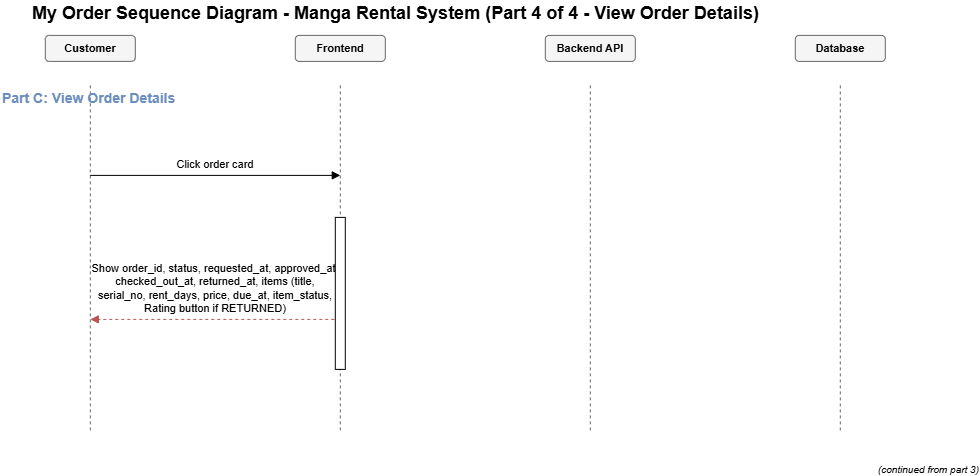
\includegraphics[width=0.85\textwidth]{images/4image78.png}
\caption{My Order Sequence Diagram - Manga Rental System (Part 4 of 4 - View Order Details)}
\label{fig:ch4_78}
\end{figure}

ภาพที่ \ref{fig:ch4_75}--\ref{fig:ch4_78} แสดง Sequence Diagram ของกระบวนการจัดการประวัติการเช่า โดยครอบคลุม 3 ฟังก์ชันหลัก ได้แก่ การดูรายการคำสั่งเช่าทั้งหมดของผู้ใช้พร้อมสถานะ กระบวนการยกเลิกคำสั่งเช่าซึ่งประกอบด้วยการตรวจสอบสถานะคำสั่งเช่า อัปเดตสถานะเป็น "ยกเลิก" และปรับสถานะหนังสือกลับเป็น "ว่าง" และการดูรายละเอียดคำสั่งเช่าแต่ละรายการพร้อมข้อมูลหนังสือที่เช่า 

\begin{figure}[H]
\centering
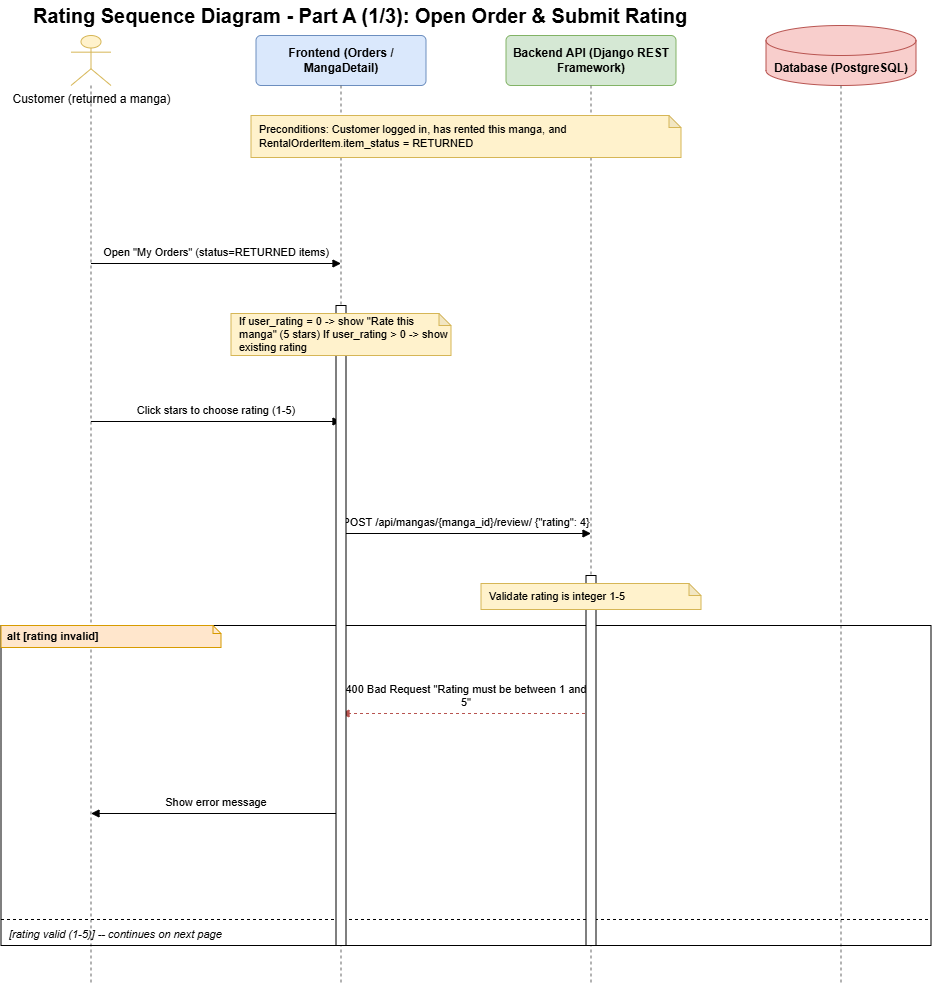
\includegraphics[width=0.85\textwidth]{images/4image79.png}
\caption{Rating Sequence Diagram - Part A (1/3): Open Order \& Submit Rating}
\label{fig:ch4_79}
\end{figure}

\begin{figure}[H]
\centering
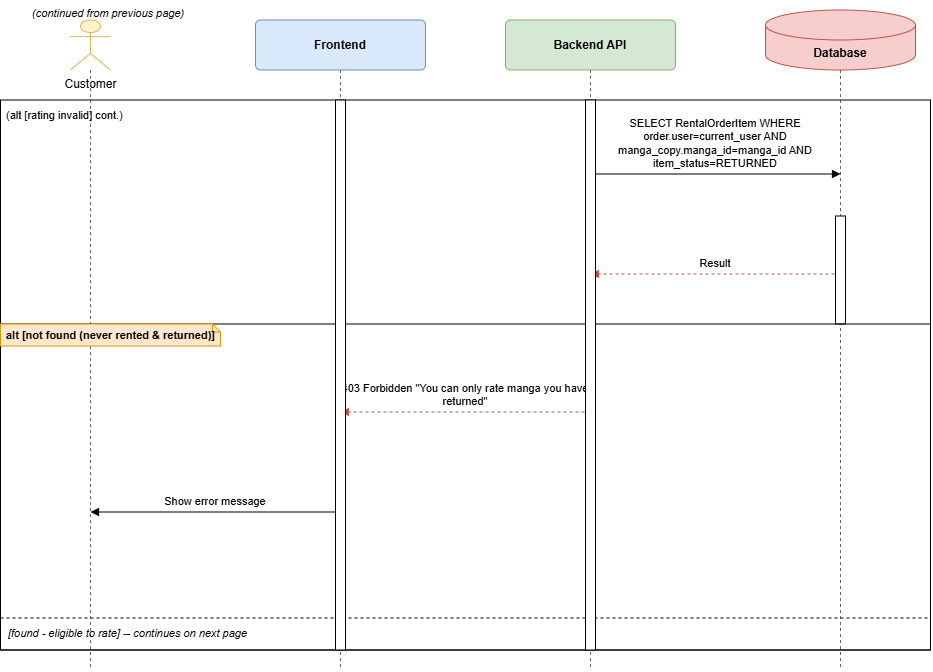
\includegraphics[width=0.85\textwidth]{images/4image80.png}
\caption{Rating Sequence Diagram - Part A (2/3): Check Eligibility}
\label{fig:ch4_80}
\end{figure}

\begin{figure}[H]
\centering
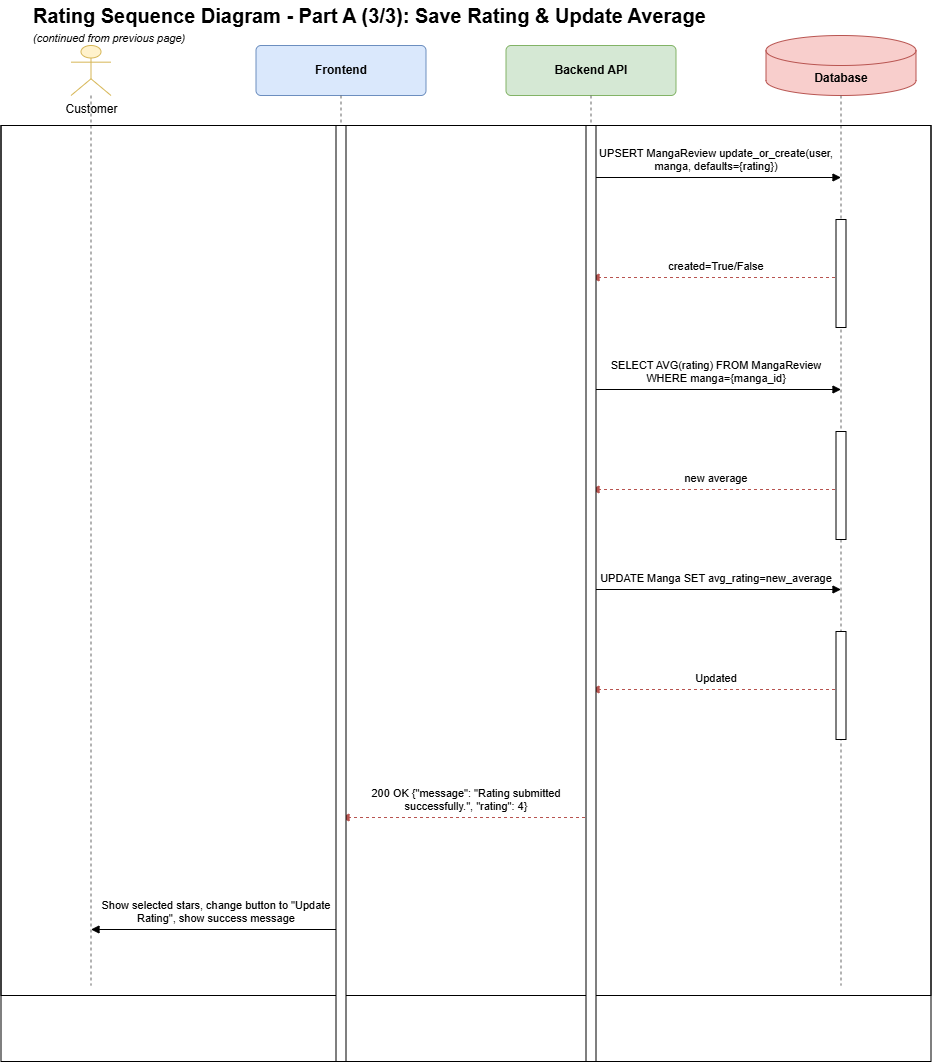
\includegraphics[width=0.85\textwidth]{images/4image81.png}
\caption{Rating Sequence Diagram - Part A (3/3): Save Rating \& Update Average}
\label{fig:ch4_81}
\end{figure}

\begin{figure}[H]
\centering
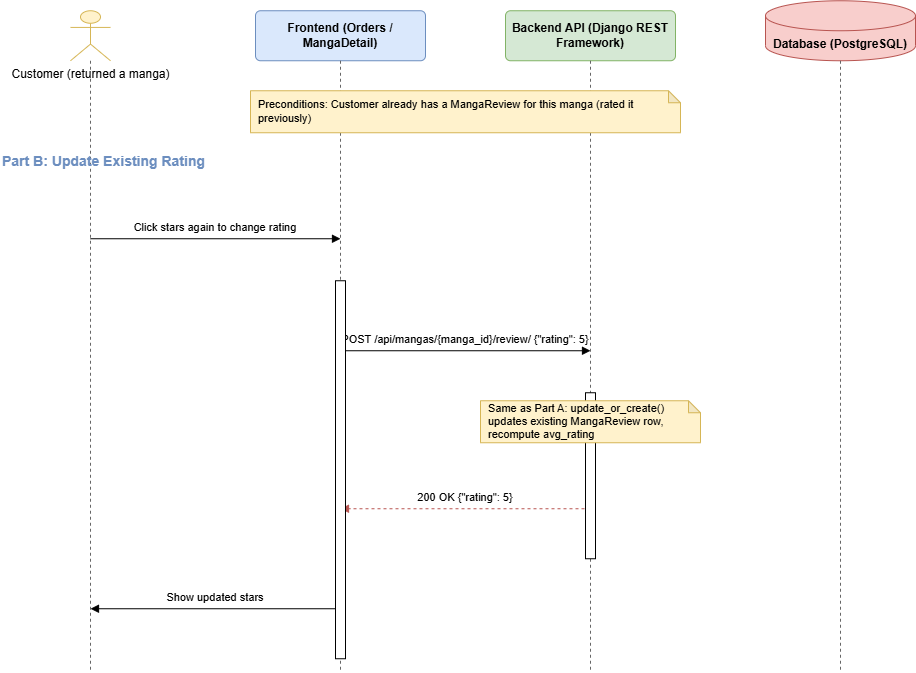
\includegraphics[width=0.85\textwidth]{images/4image82.png}
\caption{Rating Sequence Diagram - Part B: Update Existing Rating}
\label{fig:ch4_82}
\end{figure}

ภาพที่ \ref{fig:ch4_79}--\ref{fig:ch4_82} แสดง Sequence Diagram ของกระบวนการให้คะแนนและรีวิวหนังสือ แบ่งเป็น 2 กรณี คือ การให้คะแนนครั้งแรก ซึ่งระบบจะตรวจสอบสิทธิ์ว่าผู้ใช้เคยเช่าหนังสือเล่มนี้หรือไม่ หากผ่านจะบันทึกคะแนนและคำนวณคะแนนเฉลี่ยใหม่ของหนังสือ และการแก้ไขคะแนนที่เคยให้ไว้แล้ว ซึ่งระบบจะอัปเดตคะแนนเดิมและคำนวณคะแนนเฉลี่ยใหม่อีกครั้ง

\begin{figure}[H]
\centering
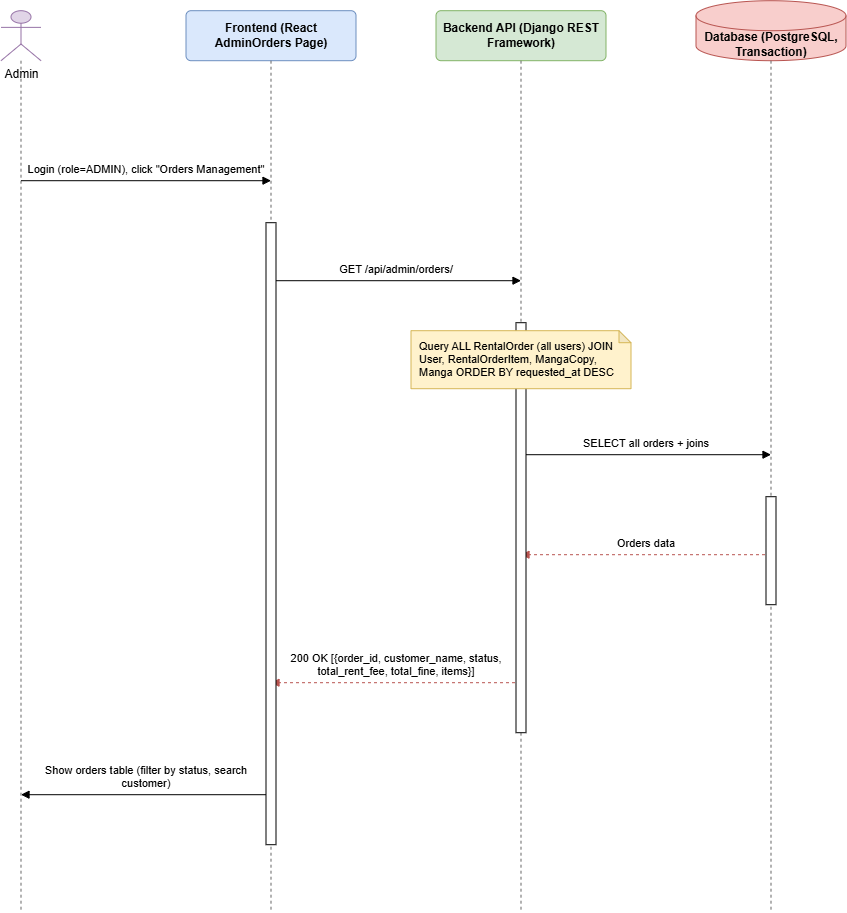
\includegraphics[width=0.85\textwidth]{images/4image83.png}
\caption{Admin Checkout Sequence Diagram - Part A: View All Orders}
\label{fig:ch4_83}
\end{figure}

\begin{figure}[H]
\centering
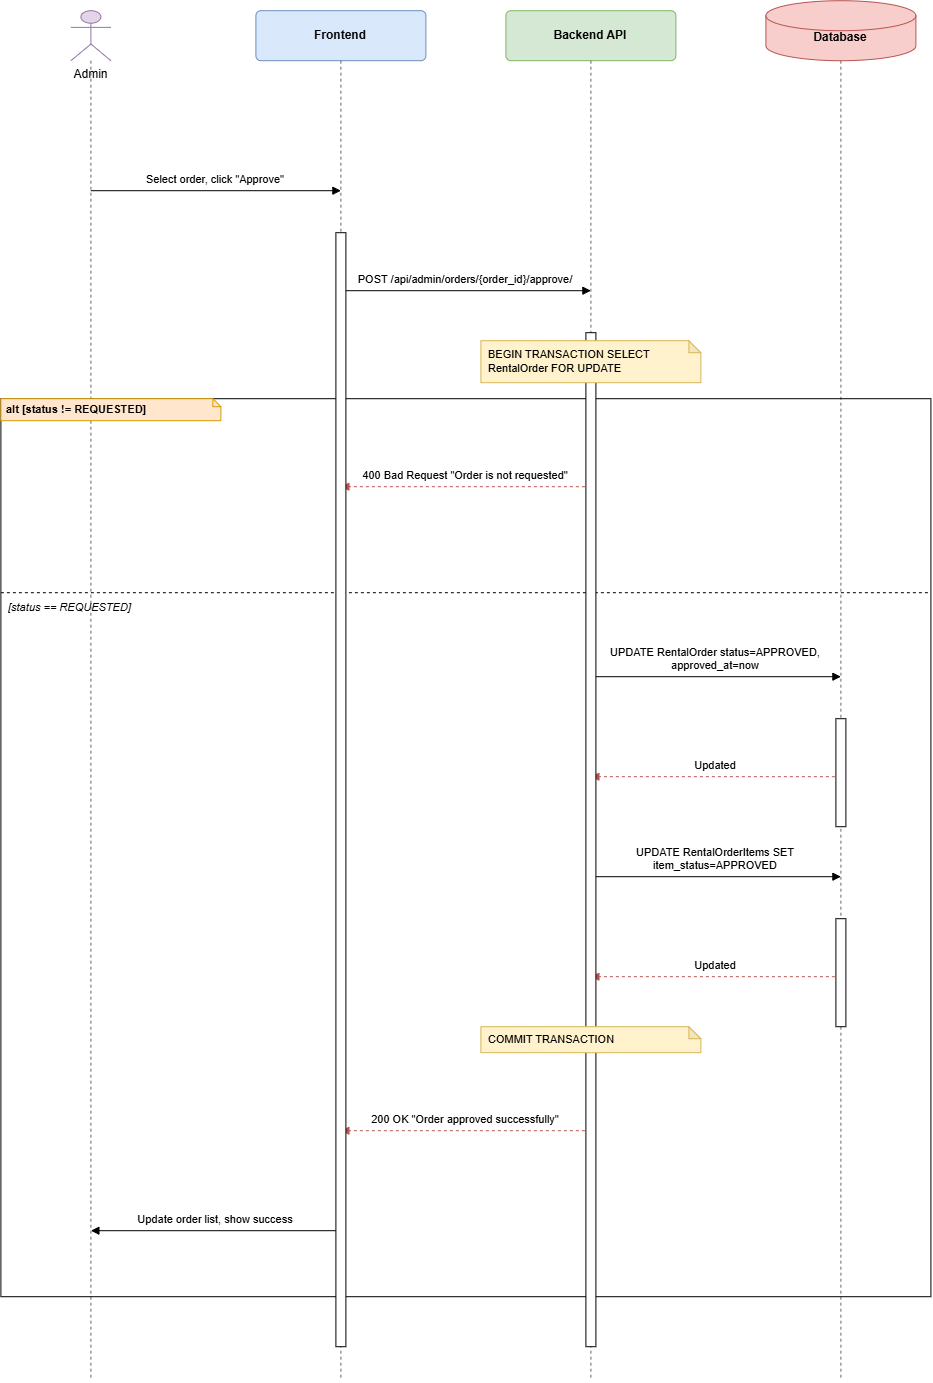
\includegraphics[width=0.85\textwidth]{images/4image84.png}
\caption{Admin Checkout Sequence Diagram - Part B: Approve Order}
\label{fig:ch4_84}
\end{figure}

\begin{figure}[H]
\centering
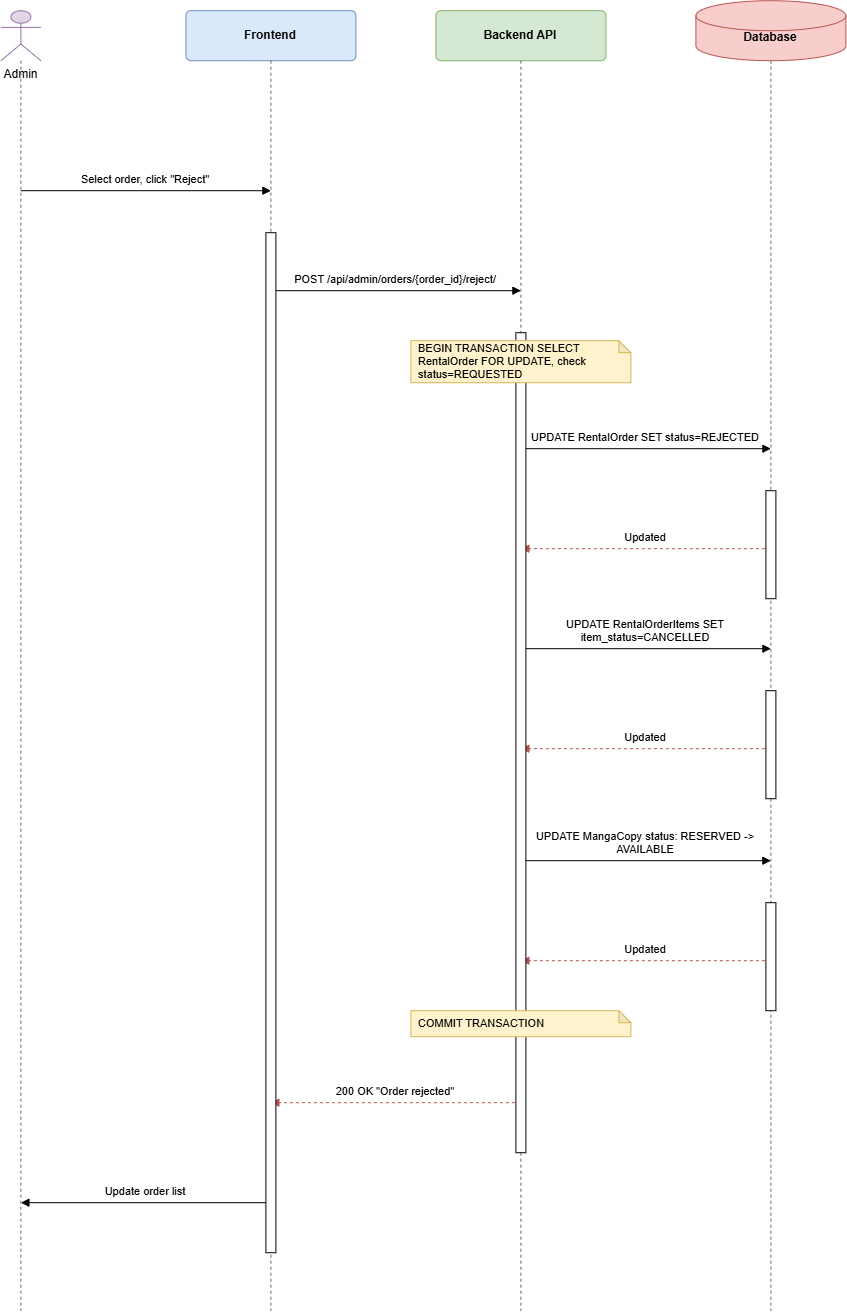
\includegraphics[width=0.85\textwidth]{images/4image85.png}
\caption{Admin Checkout Sequence Diagram - Part C: Reject Order}
\label{fig:ch4_85}
\end{figure}

\begin{figure}[H]
\centering
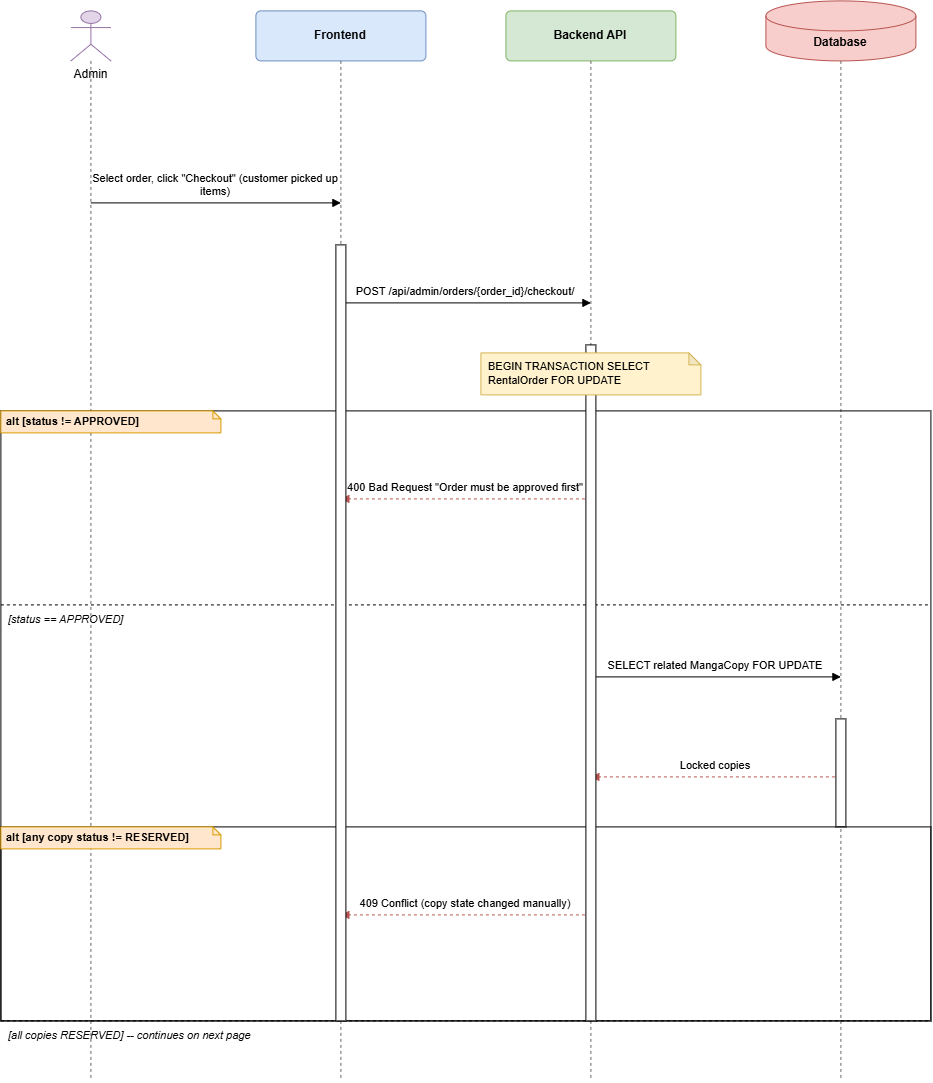
\includegraphics[width=0.85\textwidth]{images/4image86.png}
\caption{Admin Checkout Sequence Diagram - Part D (1/2): Checkout - Validation}
\label{fig:ch4_86}
\end{figure}

\begin{figure}[H]
\centering
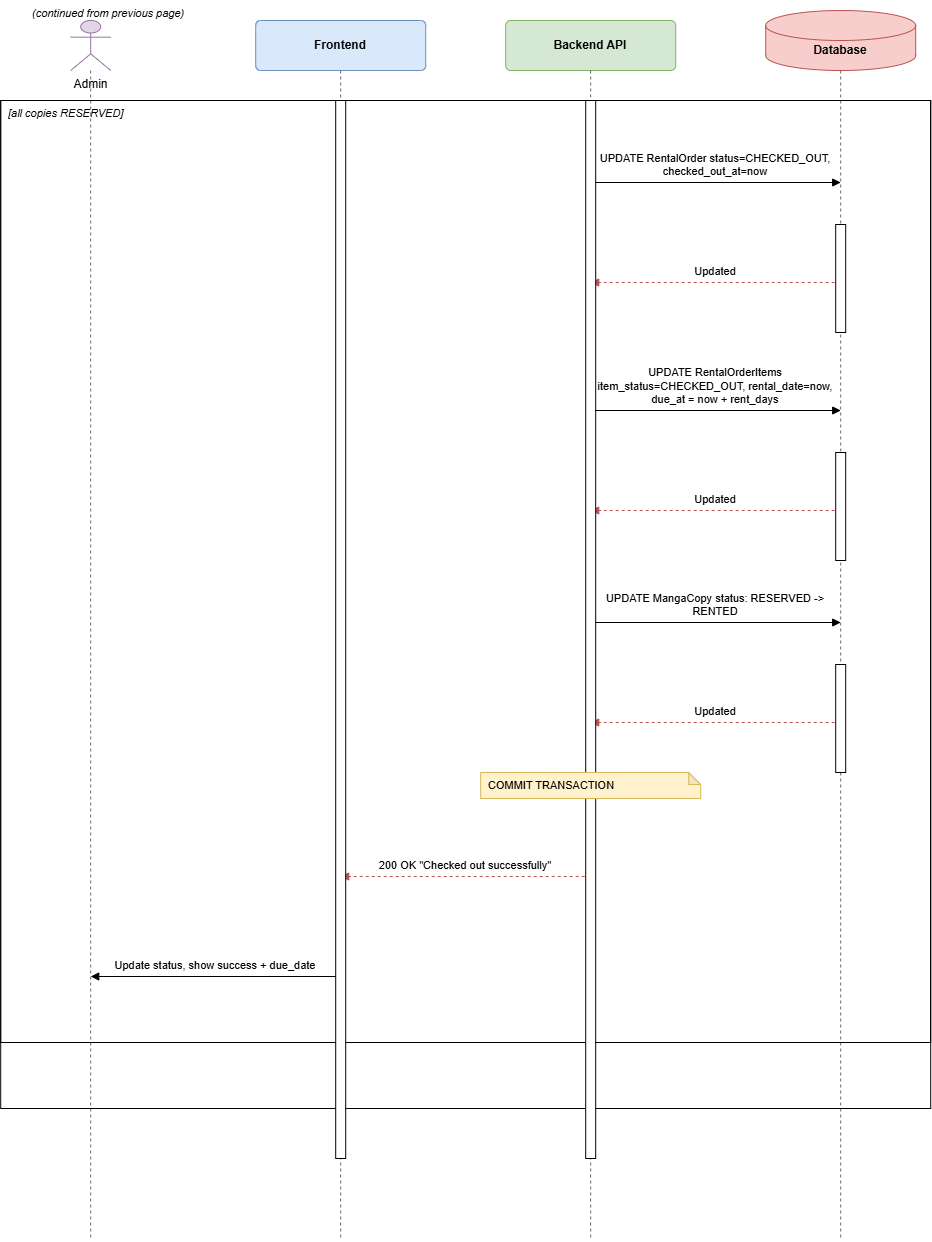
\includegraphics[width=0.85\textwidth]{images/4image87.png}
\caption{Admin Checkout Sequence Diagram - Part D (2/2): Checkout - Commit \& Response}
\label{fig:ch4_87}
\end{figure}

ภาพที่ \ref{fig:ch4_83}--\ref{fig:ch4_87} แสดง Sequence Diagram ของกระบวนการจัดการคำสั่งเช่าโดยผู้ดูแลระบบ ประกอบด้วย การดูรายการคำสั่งเช่าทั้งหมด การอนุมัติคำสั่งเช่าซึ่งจะอัปเดตสถานะเป็น "อนุมัติ" การปฏิเสธคำสั่งเช่าซึ่งจะอัปเดตสถานะเป็น "ปฏิเสธ" และปรับสถานะหนังสือกลับเป็น "ว่าง" และกระบวนการคืนหนังสือ ซึ่งตรวจสอบสภาพหนังสือและระยะเวลาการคืน คำนวณค่าปรับหากมี บันทึกข้อมูลการคืน และอัปเดตสถานะหนังสือเป็น "ว่าง"

\begin{figure}[H]
\centering
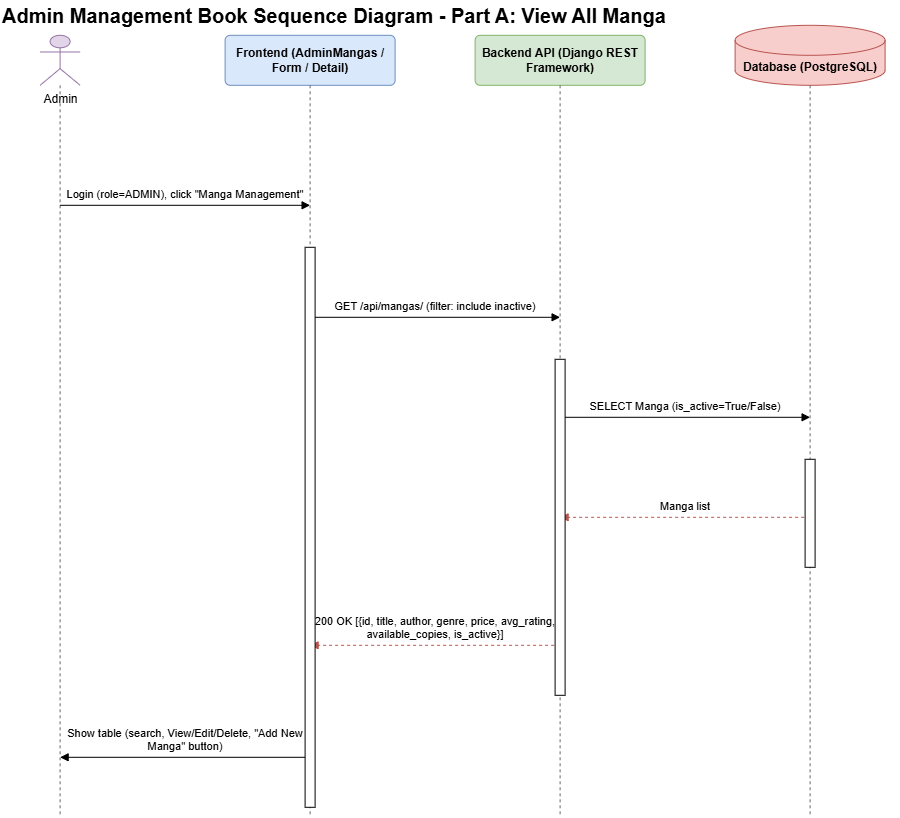
\includegraphics[width=0.85\textwidth]{images/4image88.png}
\caption{Admin Management Book Sequence Diagram - Part A: View All Manga}
\label{fig:ch4_88}
\end{figure}

\begin{figure}[H]
\centering
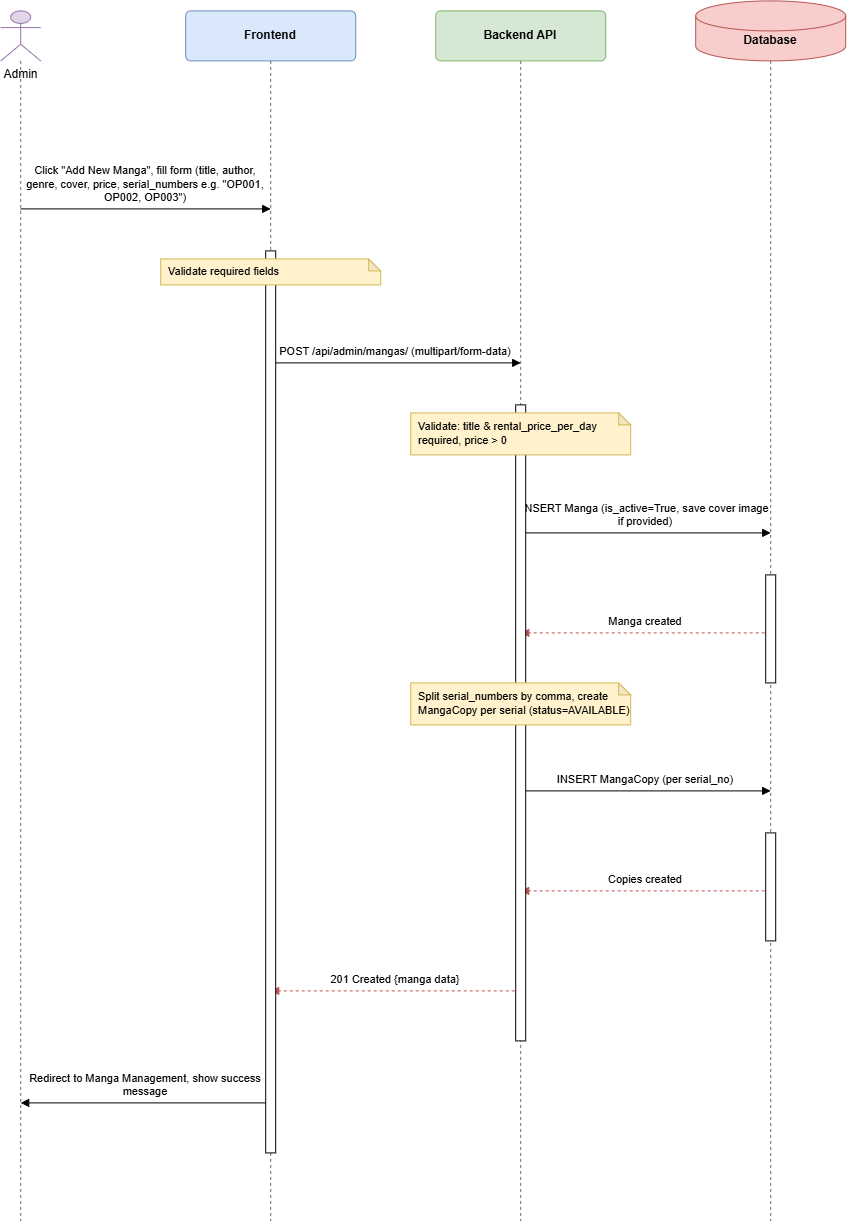
\includegraphics[width=0.85\textwidth]{images/4image89.png}
\caption{Admin Management Book Sequence Diagram - Part B: Add New Manga}
\label{fig:ch4_89}
\end{figure}

\begin{figure}[H]
\centering
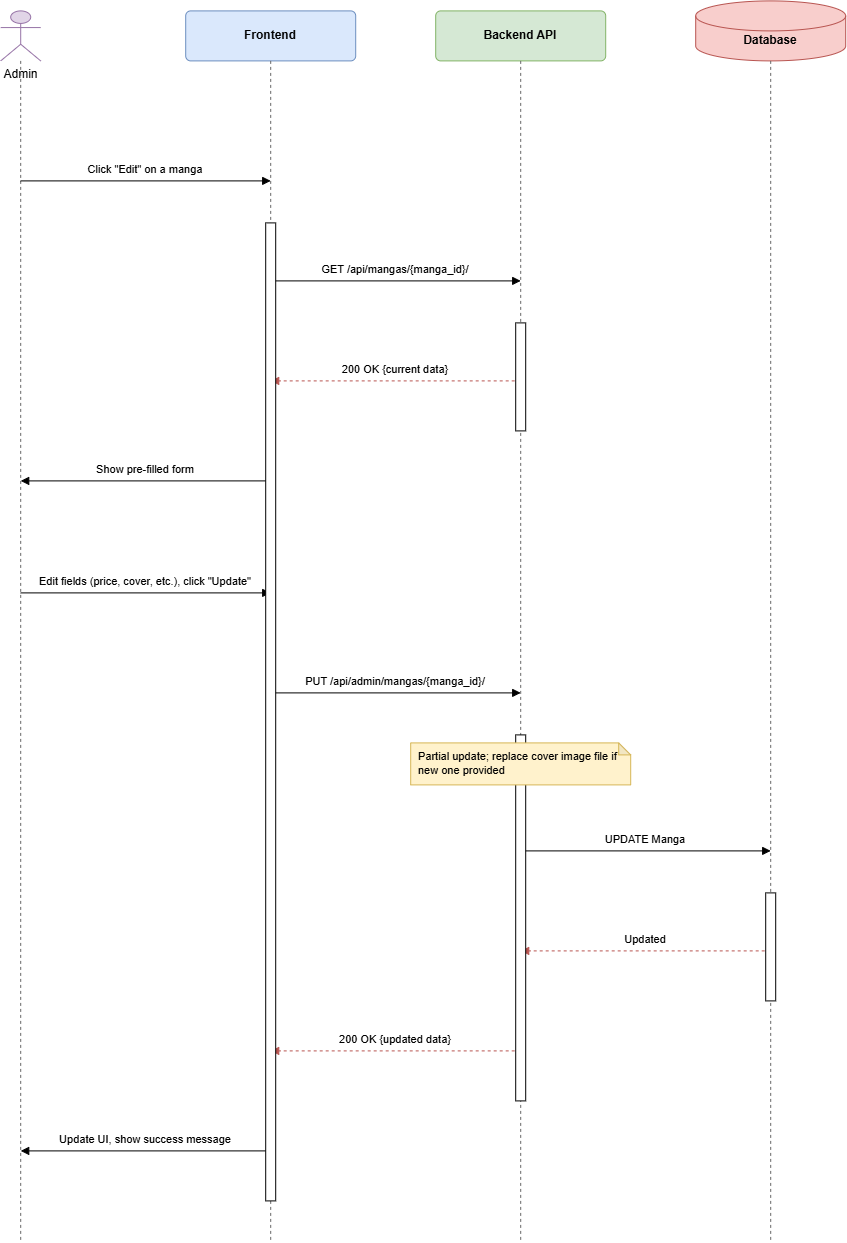
\includegraphics[width=0.85\textwidth]{images/4image90.png}
\caption{Admin Management Book Sequence Diagram - Part C: Edit Manga}
\label{fig:ch4_90}
\end{figure}

\begin{figure}[H]
\centering
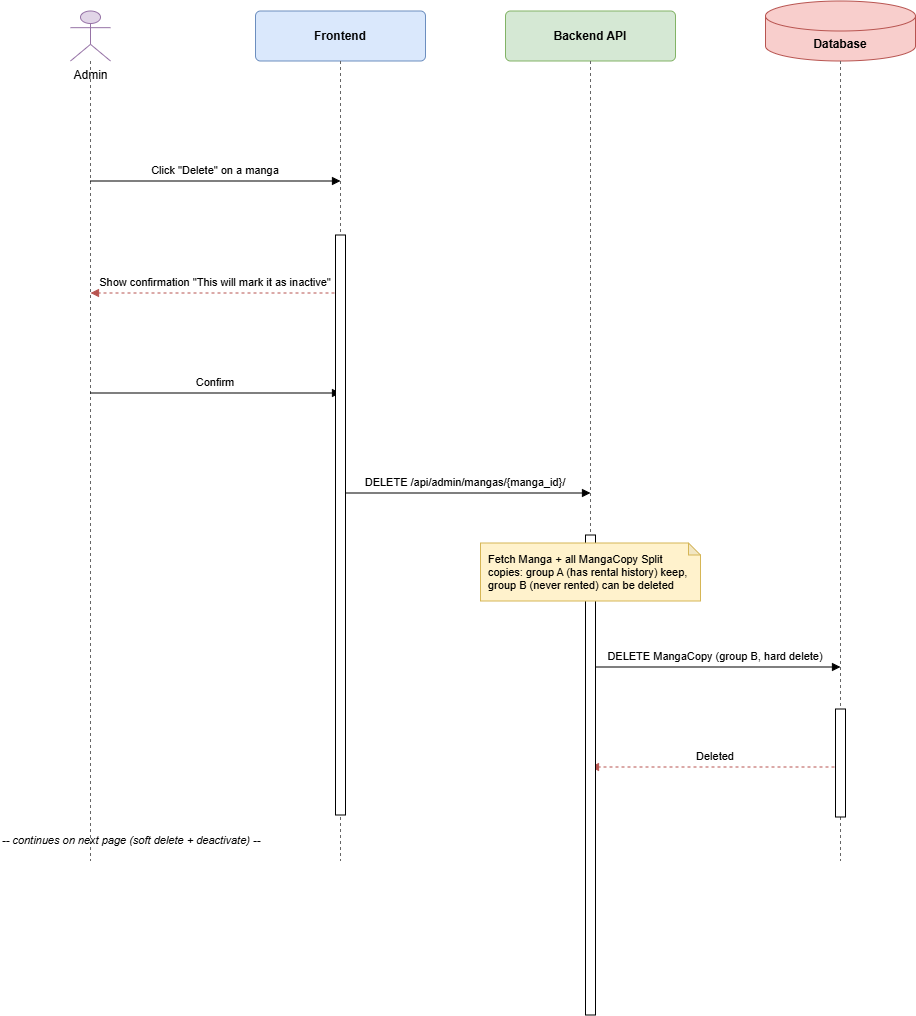
\includegraphics[width=0.85\textwidth]{images/4image91.png}
\caption{Admin Management Book Sequence Diagram - Part D (1/2): Delete/Deactivate Manga}
\label{fig:ch4_91}
\end{figure}

\begin{figure}[H]
\centering
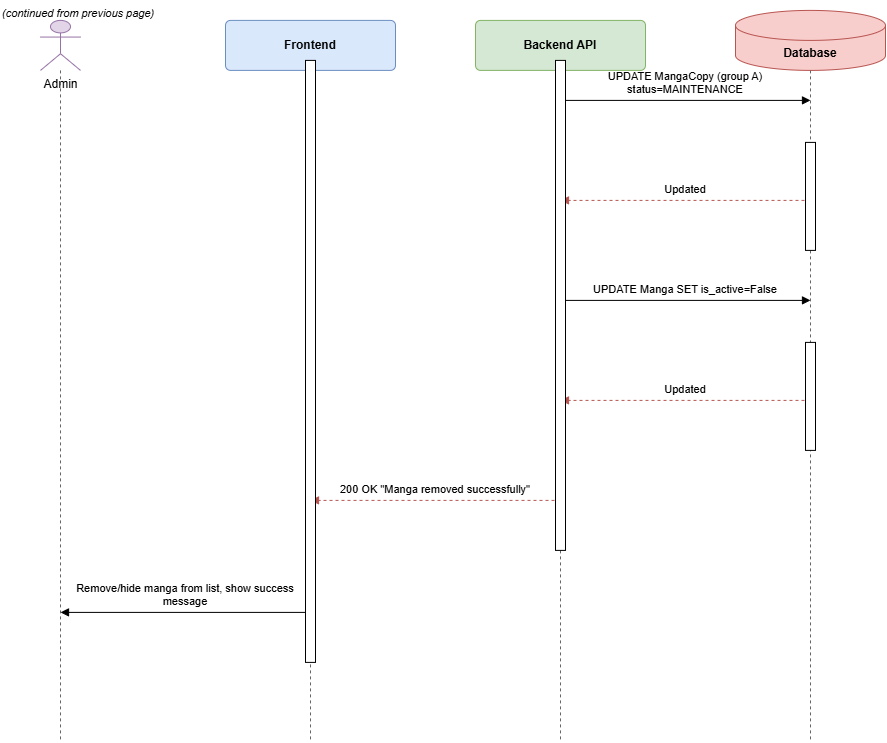
\includegraphics[width=0.85\textwidth]{images/4image92.png}
\caption{Admin Management Book Sequence Diagram - Part D (2/2): Delete/Deactivate Manga}
\label{fig:ch4_92}
\end{figure}

\begin{figure}[H]
\centering
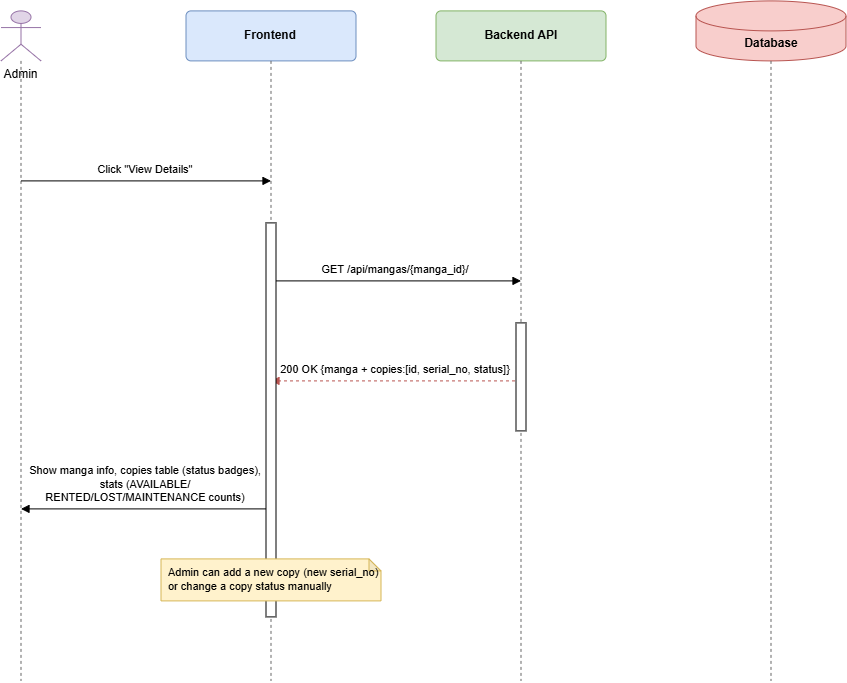
\includegraphics[width=0.85\textwidth]{images/4image93.png}
\caption{Admin Management Book Sequence Diagram - Part E: View Manga Detail \& Copies}
\label{fig:ch4_93}
\end{figure}

ภาพที่ \ref{fig:ch4_88}--\ref{fig:ch4_93} แสดง Sequence Diagram ของกระบวนการจัดการหนังสือการ์ตูนโดยผู้ดูแลระบบ ประกอบด้วย การดูรายการหนังสือทั้งหมด การเพิ่มหนังสือใหม่พร้อมอัปโหลดรูปภาพและรายละเอียด  การแก้ไขข้อมูลหนังสือที่มีอยู่ การลบหรือปิดการใช้งานหนังสือซึ่งระบบจะตรวจสอบว่ามีคำสั่งเช่าที่ใช้งานอยู่หรือไม่ก่อนทำการลบ และการดูรายละเอียดหนังสือพร้อมจำนวนสำเนาที่มีอยู่ 

\begin{figure}[H]
\centering
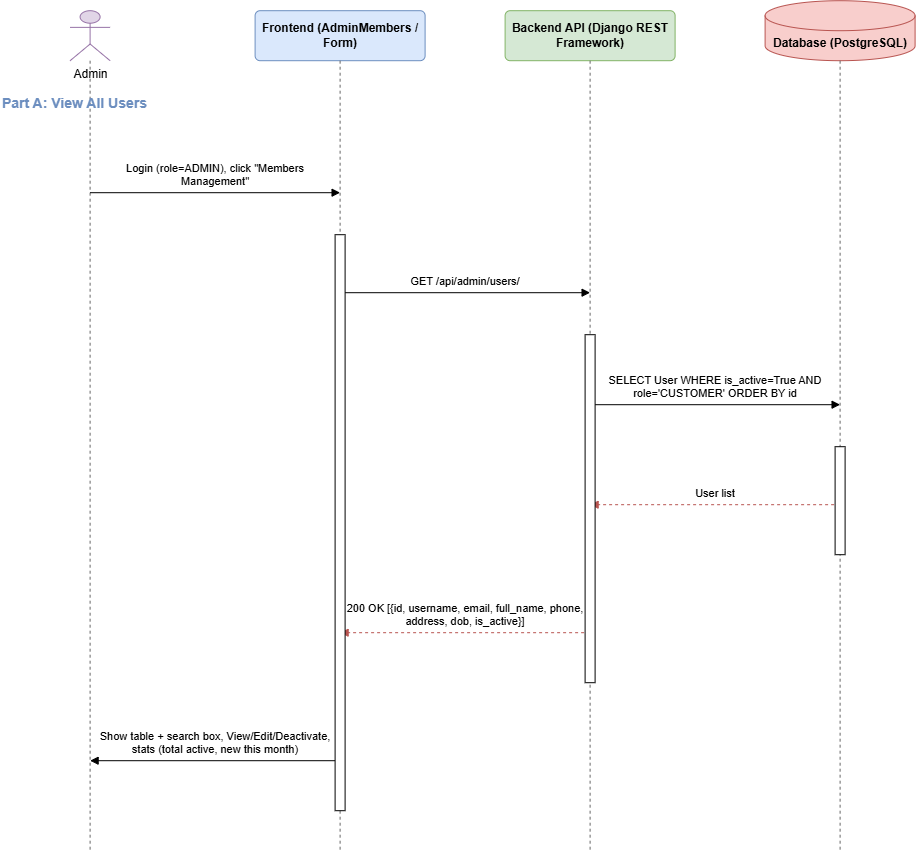
\includegraphics[width=0.85\textwidth]{images/4image94.png}
\caption{Admin Management User Sequence Diagram - Manga Rental System Part A}
\label{fig:ch4_94}
\end{figure}

\begin{figure}[H]
\centering
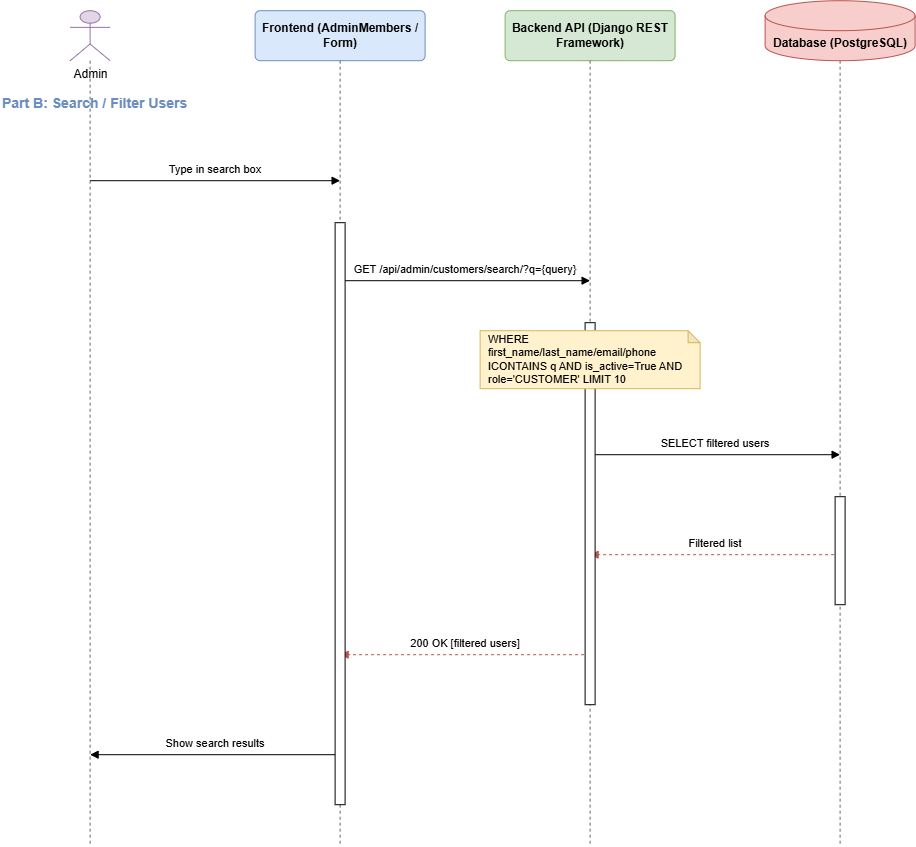
\includegraphics[width=0.85\textwidth]{images/4image95.png}
\caption{Admin Management User Sequence Diagram - Manga Rental System Part B}
\label{fig:ch4_95}
\end{figure}

\begin{figure}[H]
\centering
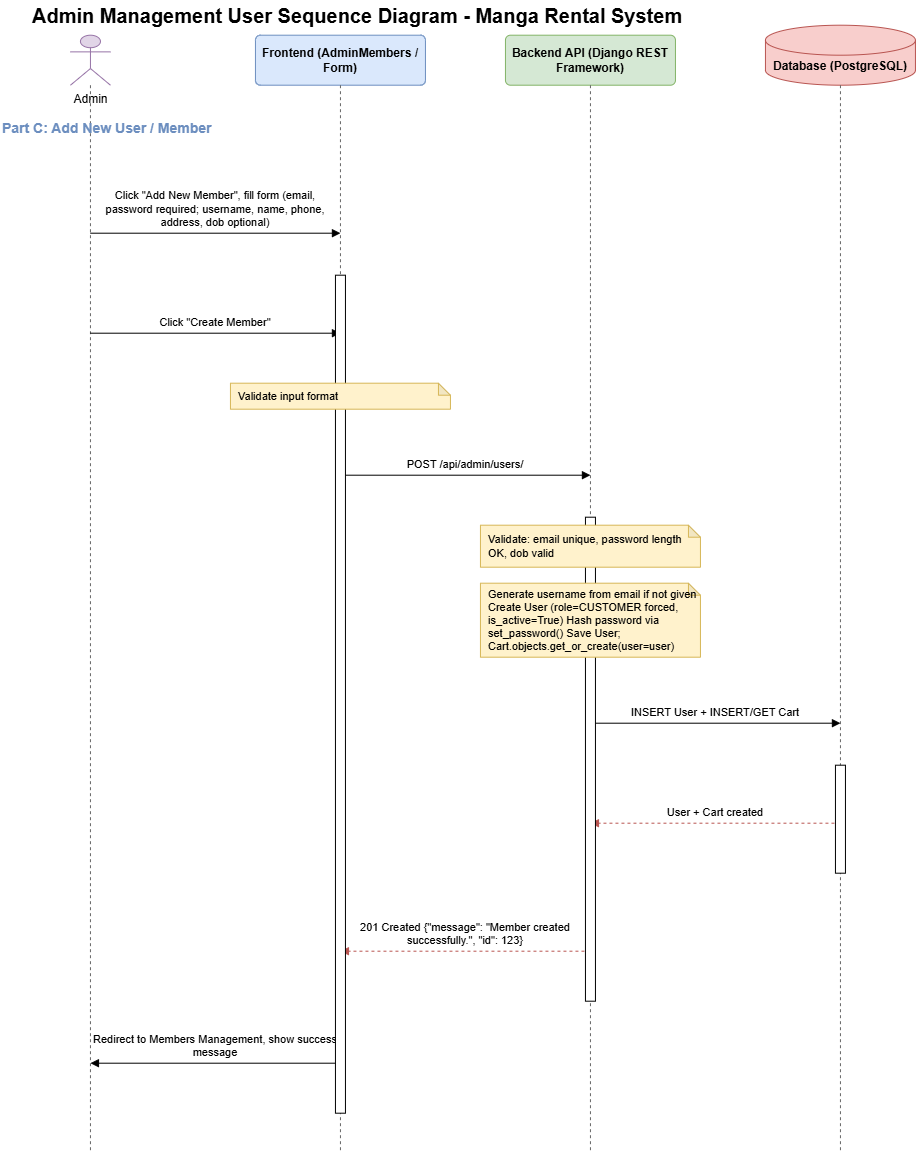
\includegraphics[width=0.85\textwidth]{images/4image96.png}
\caption{Admin Management User Sequence Diagram - Manga Rental System Part C}
\label{fig:ch4_96}
\end{figure}

\begin{figure}[H]
\centering
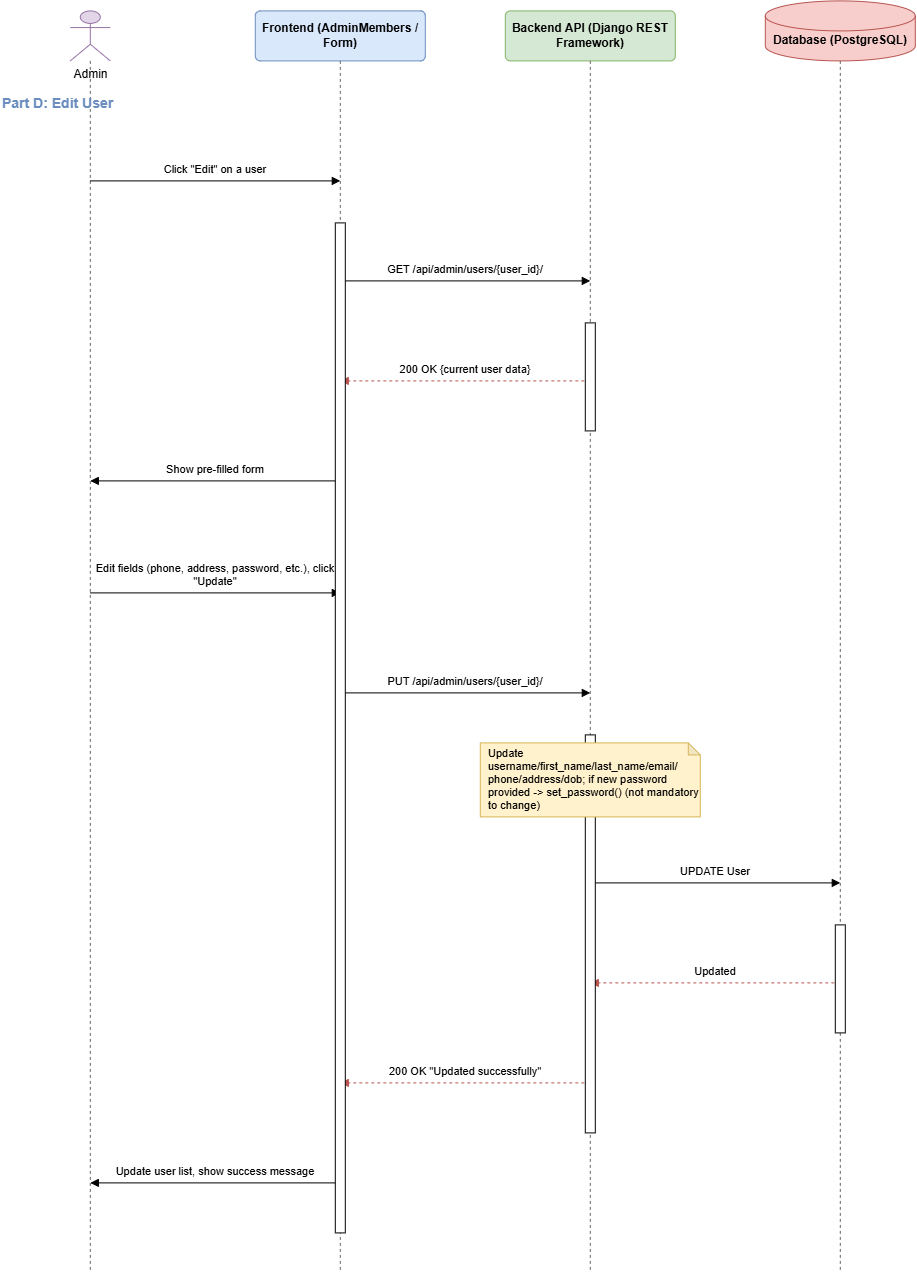
\includegraphics[width=0.85\textwidth]{images/4image97.png}
\caption{Admin Management User Sequence Diagram - Manga Rental System Part D}
\label{fig:ch4_97}
\end{figure}

\begin{figure}[H]
\centering
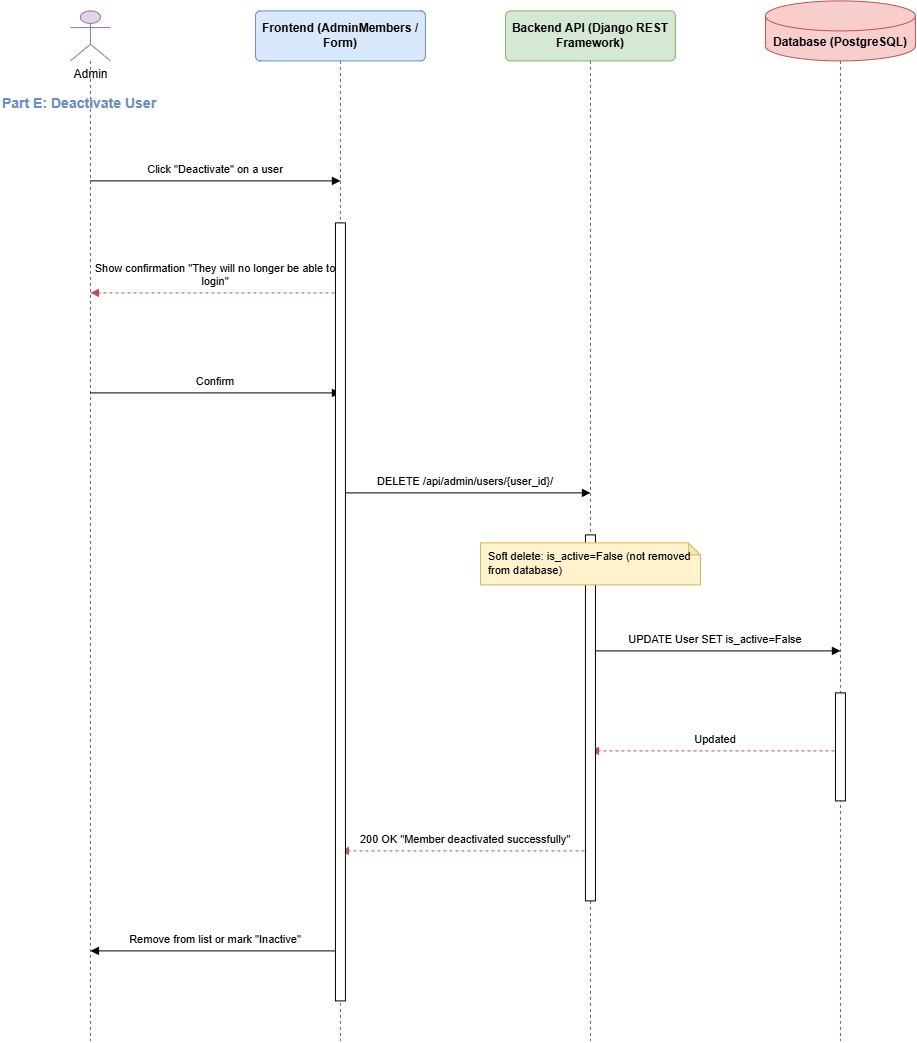
\includegraphics[width=0.85\textwidth]{images/4image98.png}
\caption{Admin Management User Sequence Diagram - Manga Rental System Part E}
\label{fig:ch4_98}
\end{figure}

\begin{figure}[H]
\centering
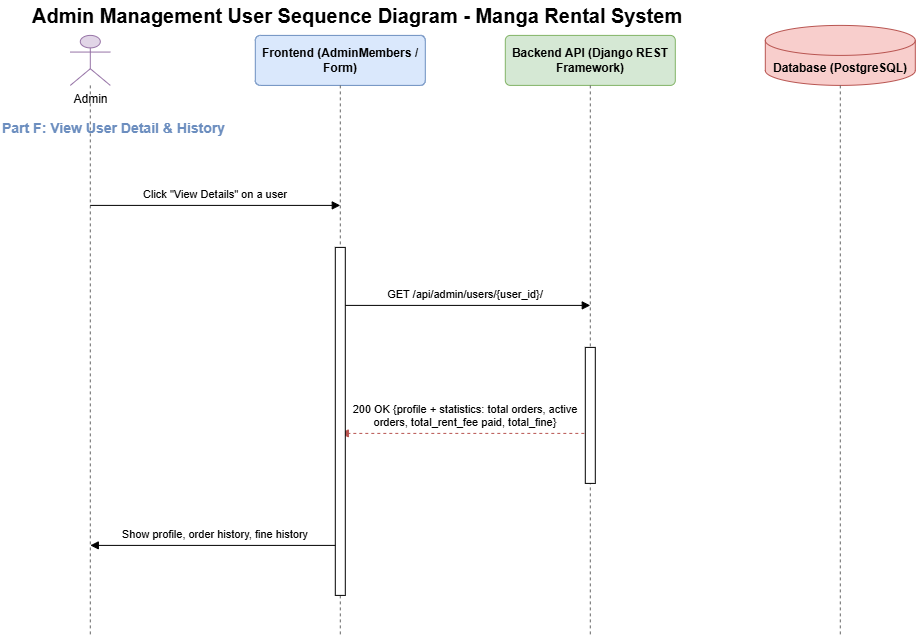
\includegraphics[width=0.85\textwidth]{images/4image99.png}
\caption{Admin Management User Sequence Diagram - Manga Rental System Part F}
\label{fig:ch4_99}
\end{figure}

\begin{figure}[H]
\centering
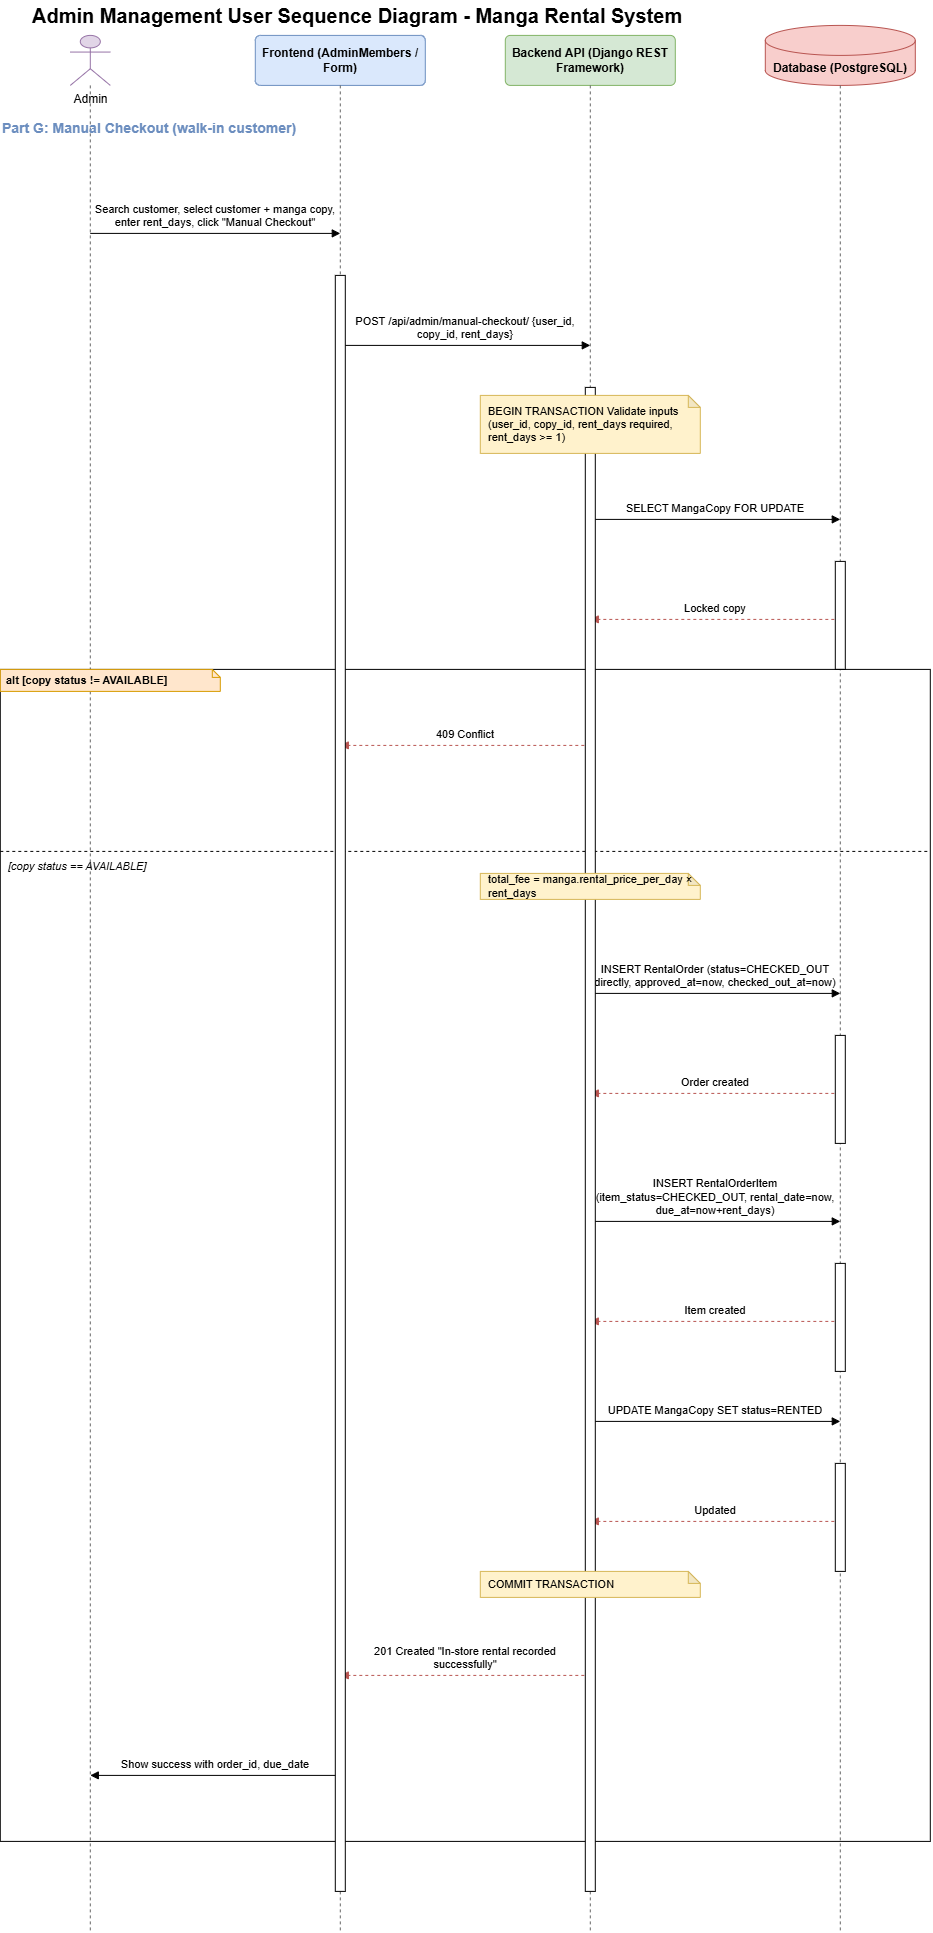
\includegraphics[width=0.7\textwidth]{images/4image100.png}
\caption{Admin Management User Sequence Diagram - Manga Rental System Part G}
\label{fig:ch4_100}
\end{figure}

ภาพที่ \ref{fig:ch4_94}--\ref{fig:ch4_100} แสดง Sequence Diagram ของกระบวนการจัดการผู้ใช้โดยผู้ดูแลระบบ ครอบคลุมฟังก์ชันการดูรายการผู้ใช้ทั้งหมด การค้นหาผู้ใช้ การดูรายละเอียดผู้ใช้แต่ละราย การแก้ไขข้อมูลผู้ใช้ การระงับหรือเปิดใช้งานบัญชีผู้ใช้ และการจัดการสิทธิ์การเข้าถึงระบบ ซึ่งผู้ดูแลระบบสามารถควบคุมและดูแลบัญชีผู้ใช้ทั้งหมดภายในระบบได้

\subsection{แผนภาพสถาปัตยกรรมระบบ}

แผนภาพสถาปัตยกรรมของระบบแสดงในภาพที่ \ref{fig:ch4_17}

\begin{figure}[H]
\centering
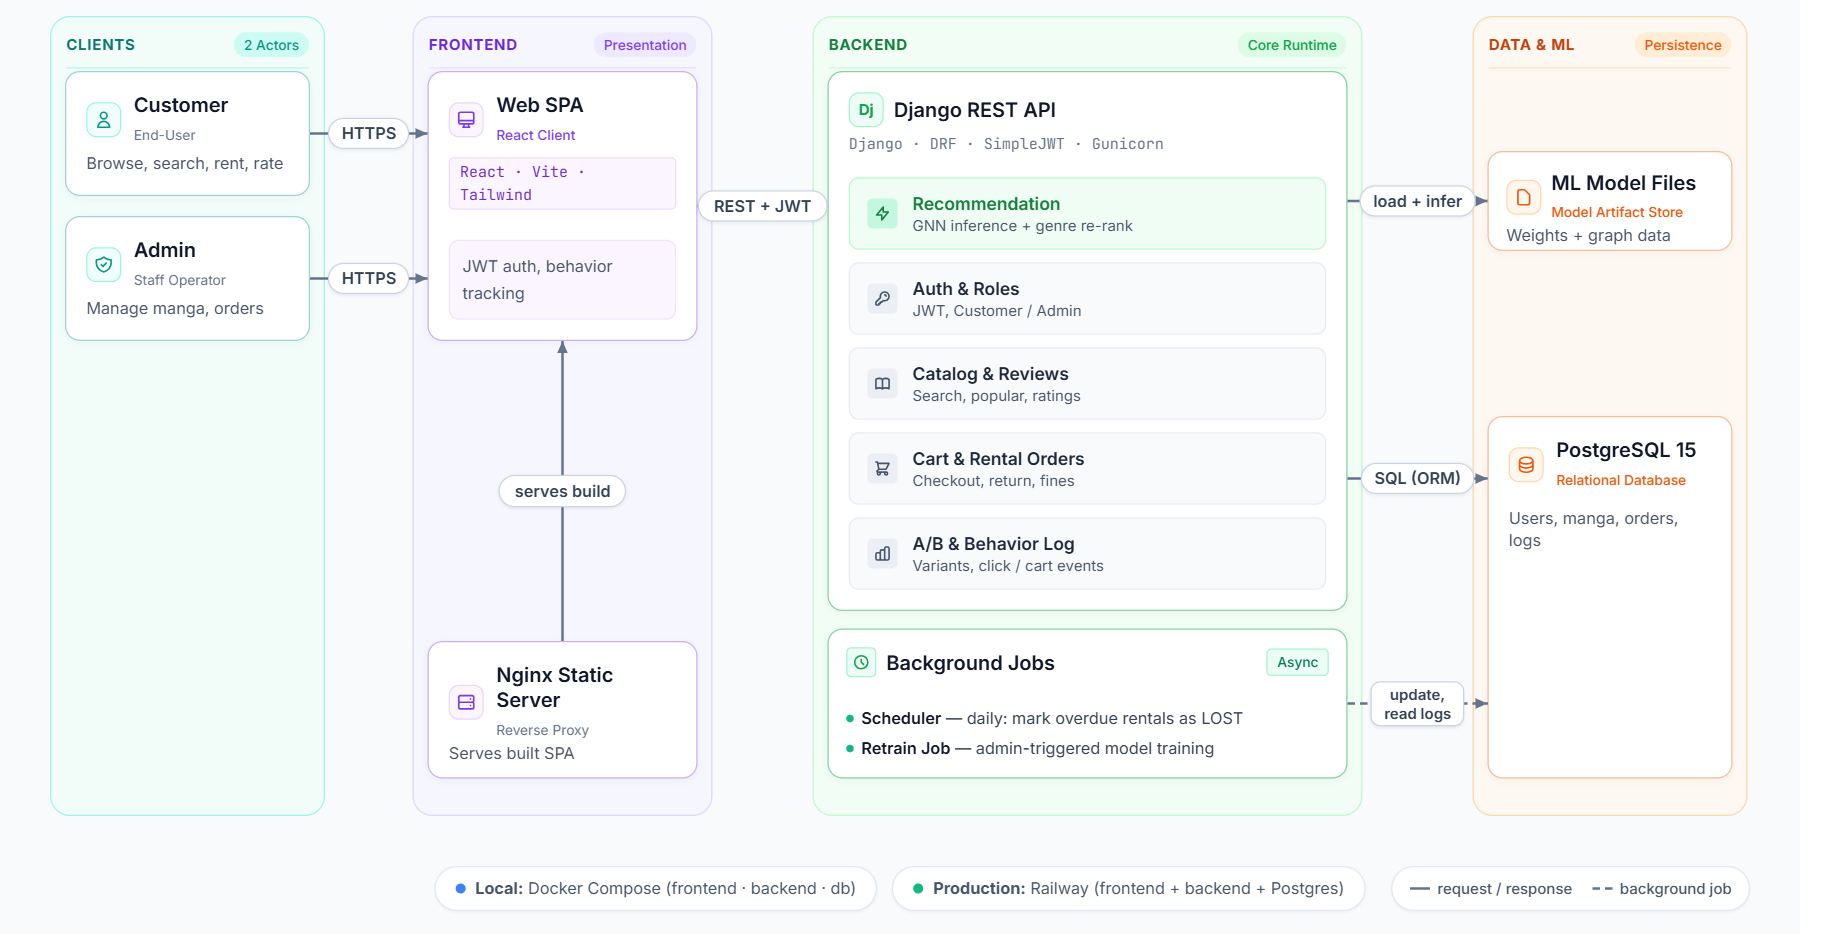
\includegraphics[width=0.9\textwidth]{images/4image17.png}
\caption{System Architecture Diagram}
\label{fig:ch4_17}
\end{figure}

ภาพที่ \ref{fig:ch4_17} ระบบแบ่งออกเป็น 4 ชั้น ผู้ใช้ทั้งกลุ่มลูกค้าและผู้ดูแลระบบเข้าใช้งานผ่านเว็บแอป (React, Vite, Tailwind) ซึ่งเสิร์ฟด้วย Nginx และสื่อสารกับ Backend ผ่าน REST API พร้อมการยืนยันตัวตนด้วย JWT ส่วน Backend พัฒนาด้วย Django REST Framework ประกอบด้วยโมดูลหลัก 5 ส่วน ได้แก่ ระบบแนะนำ (MB-CGCN), การยืนยันตัวตนและสิทธิ์, แคตตาล็อกและรีวิว, ตะกร้าและคำสั่งเช่า, และการทดสอบ A/B พร้อมบันทึกพฤติกรรมผู้ใช้ นอกจากนี้มีงานเบื้องหลัง (Background Jobs) ได้แก่ ตัวตั้งเวลาที่ตรวจรายการเช่าเกินกำหนดทุกเที่ยงคืน และงานฝึกโมเดลใหม่ที่ผู้ดูแลระบบสั่งได้ ข้อมูลทั้งหมดจัดเก็บใน PostgreSQL ส่วนโมเดลแนะนำเก็บเป็นไฟล์น้ำหนัก PyTorch ที่โหลดมาใช้ทำนายใน process เดียวกับ Backend ระบบติดตั้งด้วย Docker Compose ในเครื่องผู้พัฒนา และใช้งานจริงบน Railway

\section{การออกแบบระบบ}

\subsection{โครงสร้างฐานข้อมูล}

โครงสร้างฐานข้อมูลเชิงสัมพันธ์ของระบบแสดงดังภาพที่ \ref{fig:ch4_22}

\begin{figure}[H]
\centering
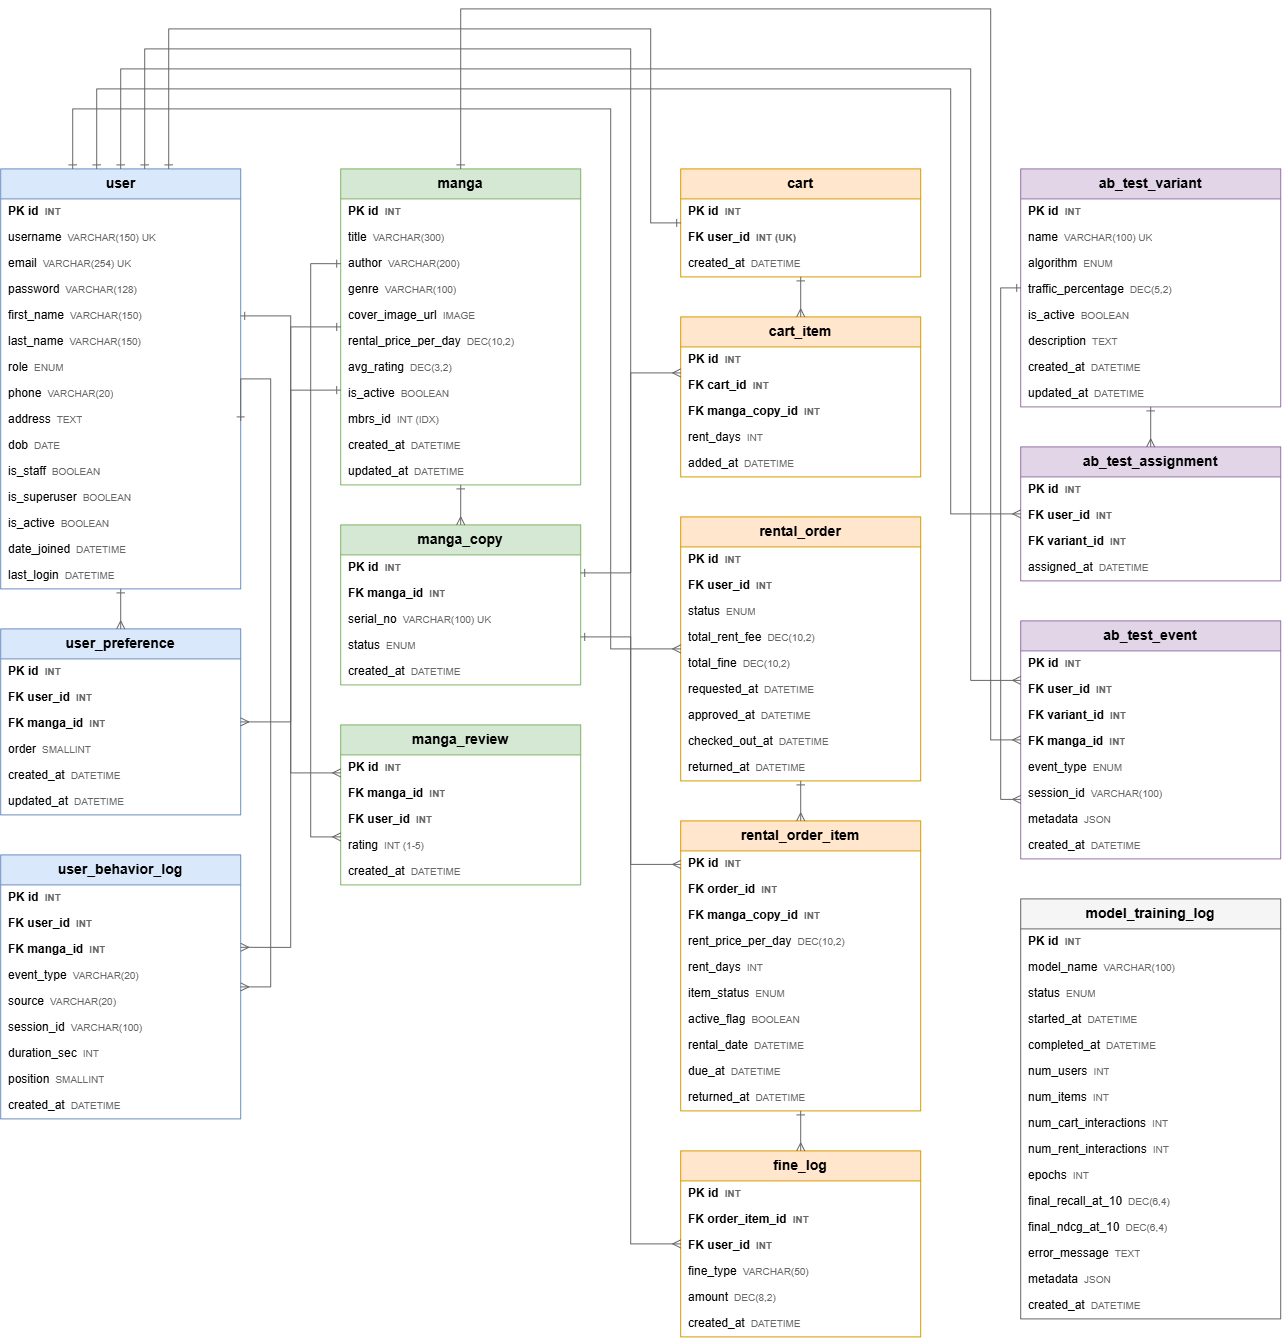
\includegraphics[width=\textwidth]{images/4image35.png}
\caption{Database Schema diagram}
\label{fig:ch4_22}
\end{figure}

ภาพที่ \ref{fig:ch4_22} แสดงโครงสร้างฐานข้อมูลเชิงสัมพันธ์ของระบบ ประกอบด้วยตารางหลักได้แก่ ตาราง Users (ข้อมูลผู้ใช้) ตาราง Manga (ข้อมูลหนังสือการ์ตูน) ตาราง MangaCopy (ข้อมูลสำเนาหนังสือแต่ละเล่ม) ตาราง Orders (คำสั่งเช่า) ตาราง OrderItems (รายการหนังสือในคำสั่งเช่า) ตาราง Cart และ CartItems (ตะกร้าสินค้า) ตาราง Ratings (คะแนนและรีวิว) และตาราง Returns (ข้อมูลการคืนหนังสือ) โดยมีความสัมพันธ์ระหว่างตารางผ่าน Foreign Key ตามหลักการออกแบบฐานข้อมูลเชิงสัมพันธ์

\section{การพัฒนาเว็บแอปพลิเคชัน}

\subsection{Technology Stack}

\subsubsection{Frontend}
React 19, React Router DOM, Vite, Tailwind CSS, PostCSS

\subsubsection{Backend}
Django 4.2+, Django REST Framework (DRF), SimpleJWT, CORS headers, Pillow, APScheduler, psycopg2-binary

\subsubsection{Machine Learning}
PyTorch, PyTorch Geometric, pandas, NumPy, scikit-learn

\subsubsection{Database}
PostgreSQL

\subsubsection{Infrastructure}
Docker Compose, Gunicorn, WhiteNoise, Nginx, Railway, Environment Variables

\subsubsection{Authentication}
JWT ผ่าน SimpleJWT (access token และ refresh token) โดยระบบใช้ค่าตั้งต้นของไลบรารี SimpleJWT ทั้งหมด ไม่มีการกำหนดค่าอายุของ Token หรือค่าอื่น ๆ เพิ่มเติมเป็นพิเศษ ดังแสดงในภาพที่ \ref{fig:ch4_101}

% TODO-IMG: แคปจาก backend/core/settings.py:140-146
\begin{figure}[H]
\centering
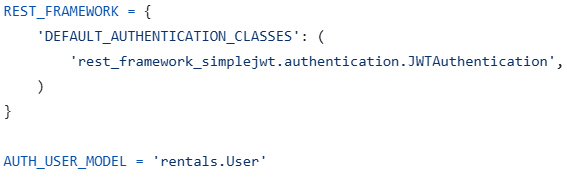
\includegraphics[width=0.85\textwidth]{images/code4_jwt_config.png}
\caption{การตั้งค่า JWT Authentication ในไฟล์ settings.py}
\label{fig:ch4_101}
\end{figure}
ภาพที่ \ref{fig:ch4_101} แสดงการตั้งค่า REST\_FRAMEWORK ในไฟล์ settings.py ซึ่งกำหนดให้ JWTAuthentication จาก SimpleJWT เป็นคลาสยืนยันตัวตนหลักของ Django REST Framework

\subsection{API Documentation}

รายการ API Endpoint ทั้งหมดของระบบแสดงดังตารางที่ \ref{tab:ch4_32}

\begingroup
\small
\begin{longtable}{|p{0.6cm}|p{1.6cm}|p{4.3cm}|p{1.9cm}|p{1.7cm}|}
\caption{API Endpoint} \label{tab:ch4_32} \\
\hline
\textbf{\#} & \textbf{Method} & \textbf{Endpoint} & \textbf{Permission} & \textbf{หมวดหมู่} \\ \hline
\endfirsthead
\caption[]{API Endpoint (ต่อ)} \\
\hline
\textbf{\#} & \textbf{Method} & \textbf{Endpoint} & \textbf{Permission} & \textbf{หมวดหมู่} \\ \hline
\endhead
1 & POST & /api/token/ & Public & Auth \\ \hline
2 & POST & /api/token/refresh/ & Public & Auth \\ \hline
3 & POST & /api/register/ & Public & Auth \\ \hline
4 & GET & /api/me/ & Authenticated & User \\ \hline
5 & GET & /api/users/profile/ & Authenticated & User \\ \hline
6 & PUT & /api/users/profile/ & Authenticated & User \\ \hline
7 & GET & /api/mangas/ & Public & Manga \\ \hline
8 & GET & /api/mangas/\{id\}/ & Public & Manga \\ \hline
9 & GET & /api/mangas/popular/ & Public & Manga \\ \hline
10 & POST & /api/mangas/\{manga\_id\}/review/ & Authenticated & Review \\ \hline
11 & GET & /api/cart/ & Authenticated & Cart \\ \hline
12 & POST & /api/cart/add/\{manga\_id\}/ & Authenticated & Cart \\ \hline
13 & DELETE & /api/cart/remove/\{item\_id\}/ & Authenticated & Cart \\ \hline
14 & POST & /api/cart/checkout/ & Authenticated & Cart \\ \hline
15 & GET & /api/orders/ & Authenticated & Order \\ \hline
16 & POST & /api/orders/\{order\_id\}/cancel/ & Authenticated & Order \\ \hline
17 & GET & /api/admin/orders/ & Admin & Admin-Order \\ \hline
18 & POST & /api/admin/orders/\{order\_id\}/approve/ & Admin & Admin-Order \\ \hline
19 & POST & /api/admin/orders/\{order\_id\}/reject/ & Admin & Admin-Order \\ \hline
20 & POST & /api/admin/orders/\{order\_id\}/checkout/ & Admin & Admin-Order \\ \hline
21 & POST & /api/admin/orders/\{order\_id\}/items/\{item\_id\}/return/ & Admin & Admin-Order \\ \hline
22 & POST & /api/admin/orders/\{order\_id\}/items/\{item\_id\}/fine/ & Admin & Admin-Order \\ \hline
23 & GET & /api/admin/users/ & Admin & Admin-User \\ \hline
24 & POST & /api/admin/users/ & Admin & Admin-User \\ \hline
25 & GET & /api/admin/users/\{user\_id\}/ & Admin & Admin-User \\ \hline
26 & PUT & /api/admin/users/\{user\_id\}/ & Admin & Admin-User \\ \hline
27 & DELETE & /api/admin/users/\{user\_id\}/ & Admin & Admin-User \\ \hline
28 & GET & /api/admin/customers/search/ & Admin & Admin-User \\ \hline
29 & POST & /api/admin/mangas/ & Admin & Admin-Manga \\ \hline
30 & PUT & /api/admin/mangas/\{manga\_id\}/ & Admin & Admin-Manga \\ \hline
31 & DELETE & /api/admin/mangas/\{manga\_id\}/ & Admin & Admin-Manga \\ \hline
32 & POST & /api/admin/manual-checkout/ & Admin & Admin-Misc \\ \hline
33 & GET & /api/admin/history/ & Admin & Admin-Misc \\ \hline
34 & GET & /api/recommendations/ & Authenticated & Recommendation \\ \hline
35 & GET, POST & /api/preferences/ & Authenticated & Preference \\ \hline
36 & POST & /api/behaviors/log/ & Authenticated & Behavior \\ \hline
37 & GET & /api/admin/behaviors/stats/ & Admin & Behavior \\ \hline
38 & GET, POST, PUT, DELETE & /api/admin/ab-test/variants/ & Admin & A/B Test \\ \hline
39 & GET & /api/admin/ab-test/metrics/ & Admin & A/B Test \\ \hline
40 & POST & /api/admin/ml/retrain/ & Admin & ML Training \\ \hline
41 & GET & /api/admin/ml/status/ & Admin & ML Training \\ \hline
42 & GET, POST & /api/admin/ml/config/ & Admin & ML Training \\ \hline
43 & POST & /api/admin/ml/training-logs/\{log\_id\}/activate/ & Admin & ML Training \\ \hline
44 & GET & /api/health/ & Public & Health \\ \hline
\end{longtable}
\endgroup


\section{การพัฒนาโมเดลระบบแนะนำ}

ในส่วนนี้จะอธิบายถึงกระบวนการทางวิศวกรรมในการพัฒนาโมเดลแนะนำหนังสือการ์ตูนแบบหลายพฤติกรรม โดยใช้สถาปัตยกรรม Multi-Behavior Cascading Graph Convolutional Networks (MB-CGCN) ที่พัฒนาขึ้นด้วยเฟรมเวิร์ก PyTorch สถาปัตยกรรมนี้อยู่ในกลุ่มโครงข่ายประสาทแบบกราฟ (Graph Convolutional Network หรือ GCN) ซึ่งเรียนรู้เวกเตอร์ตัวแทน (Embedding) ของผู้ใช้และหนังสือการ์ตูนโดยอาศัยการส่งผ่านและรวมข้อมูล (Message Passing) ระหว่างจุดที่เชื่อมต่อกันในกราฟปฏิสัมพันธ์ ซ้ำกันหลายรอบ (Convolution Layer) เพื่อให้เวกเตอร์ตัวแทนสะท้อนทั้งความสัมพันธ์โดยตรงและความสัมพันธ์ทางอ้อมผ่านจุดอื่น ๆ ในกราฟ และคำว่า ``Cascading'' หมายถึงการที่โมเดลเรียนรู้จากพฤติกรรมหลายประเภทตามลำดับขั้น โดยส่งผลลัพธ์จากการเรียนรู้พฤติกรรมหนึ่งไปเป็นจุดตั้งต้นของการเรียนรู้พฤติกรรมถัดไป ดังจะอธิบายรายละเอียดในหัวข้อต่อไป

\subsection{ชุดข้อมูลที่ใช้ในการพัฒนาโมเดล (Dataset)}

ชุดข้อมูลที่ใช้ในการฝึกสอนโมเดลประกอบด้วยไฟล์ CSV จำนวน 2 ไฟล์ ได้แก่

\subsubsection{ไฟล์ Anime.csv}
เก็บข้อมูลรายการหนังสือการ์ตูนทั้งหมดจำนวน 28,467 รายการ ประกอบด้วยคอลัมน์หลักที่ใช้งาน ได้แก่ anime\_id, name, title\_english, status และ source ที่เป็นแหล่งที่มาของเรื่อง เช่น Manga, Light novel, Original, Game เป็นต้น ตัวอย่างข้อมูลดิบบางส่วนแสดงดังภาพที่ \ref{fig:ch4_107}

% TODO-IMG: img4_anime_csv_sample.png -- capture ตัวอย่างแถวข้อมูลจาก Anime.csv ด้วย pandas.read_csv().head(15)
\begin{figure}[H]
\centering
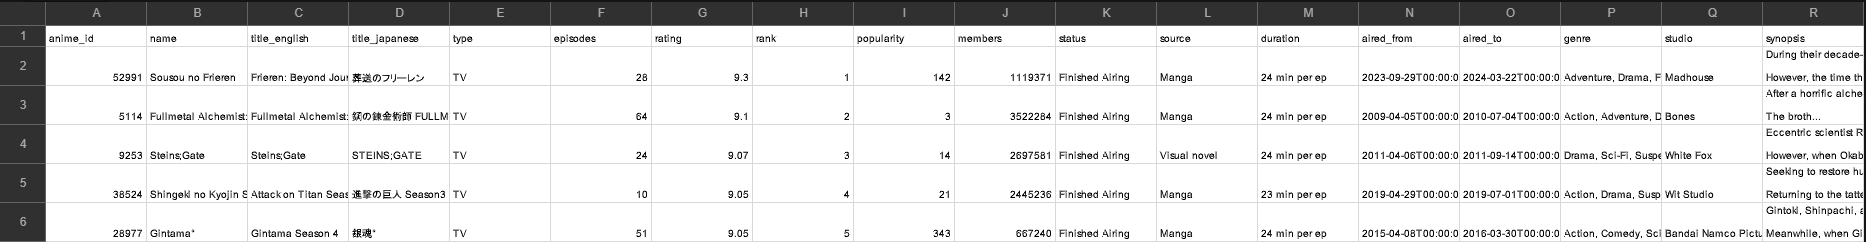
\includegraphics[width=0.85\textwidth]{images/img4_anime_csv_sample.png}
\caption{ตัวอย่างข้อมูลดิบจากไฟล์ Anime.csv}
\label{fig:ch4_107}
\end{figure}

\subsubsection{ไฟล์ User-AnimeReview.csv}
เก็บข้อมูลปฏิสัมพันธ์ระหว่างผู้ใช้กับรายการหนังสือการ์ตูนจำนวนกว่า 16.5 ล้านแถว ประกอบด้วยคอลัมน์ user\_id, anime\_id, score, status ที่เก็บสถานะการปฏิสัมพันธ์ เช่น Plan to Watch, Watching, Completed และ episodes\_seen ตัวอย่างข้อมูลดิบบางส่วนแสดงดังภาพที่ \ref{fig:ch4_108}

% TODO-IMG: img4_review_csv_sample.png -- capture ตัวอย่างแถวข้อมูลจาก User-AnimeReview.csv ด้วย pandas.read_csv().head(15)
\begin{figure}[H]
\centering
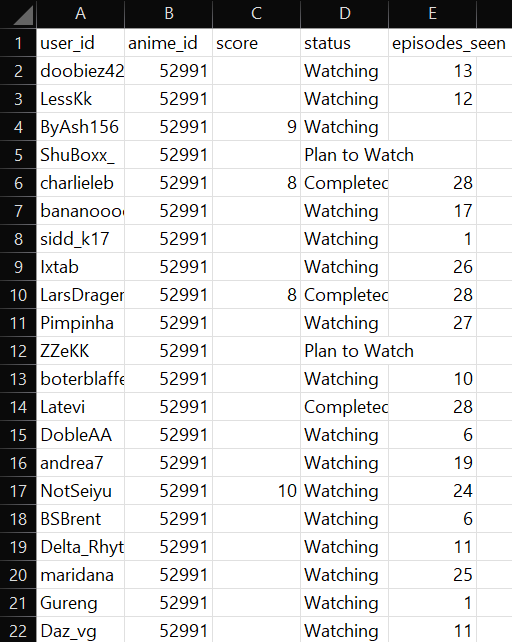
\includegraphics[width=0.85\textwidth]{images/img4_review_csv_sample.png}
\caption{ตัวอย่างข้อมูลดิบจากไฟล์ User-AnimeReview.csv}
\label{fig:ch4_108}
\end{figure}


สถาปัตยกรรมที่ออกแบบไว้สำหรับโมเดล MBRS รองรับห่วงโซ่พฤติกรรมได้ตั้งแต่ 2 ขั้นถึง 3 ขั้น โดยพฤติกรรมการเช่า ถูกกำหนดให้เป็นพฤติกรรมเป้าหมายหลักและอยู่ท้ายสุดของห่วงโซ่เสมอ ในโครงงานนี้ได้พัฒนาและทดสอบโมเดลจริง 2 เวอร์ชัน ได้แก่ โมเดลเวอร์ชัน 1 (v1) ที่ใช้ห่วงโซ่ 2 ขั้น Cart $\rightarrow$ Rent ฝึกจากข้อมูล MyAnimeList กว่า 700,000 ผู้ใช้ และโมเดลเวอร์ชัน 2 (v2) ที่ขยายเป็นห่วงโซ่ 3 ขั้น Click $\rightarrow$ Cart $\rightarrow$ Rent ฝึกจากข้อมูลพฤติกรรมจำลอง 1,000 ผู้ใช้กับหนังสือ 100 เรื่อง เพื่อทดสอบกลไกการเรียนรู้พฤติกรรมเสริมตั้งแต่ขั้นการคลิกดูรายละเอียดก่อนที่ระบบจะมีผู้ใช้จริงจำนวนมากพอ ทั้ง 2 เวอร์ชันได้ผ่านการฝึกสอนและประเมินประสิทธิภาพเสร็จสมบูรณ์แล้ว โดยผลการทดสอบของทั้งสองรุ่นจะแสดงในหัวข้อ 4.5.2 ส่วนรายละเอียดขั้นตอนการเตรียมข้อมูล สถาปัตยกรรม และการตั้งค่าพารามิเตอร์ในหัวข้อต่อไปนี้ อธิบายโดยใช้โมเดล v1 เป็นหลัก เนื่องจากเป็นโมเดลที่ฝึกจากข้อมูลจริงและใช้งานจริงในระบบเว็บแอปพลิเคชัน ขณะที่โมเดล v2 ใช้กลไกและพารามิเตอร์ชุดเดียวกัน แต่มีเลเยอร์เพิ่มเติมสำหรับพฤติกรรม Click และใช้น้ำหนักพฤติกรรมแบบปรับได้ แทนค่าคงที่ 

\subsection{การเตรียมข้อมูลและโครงสร้างข้อมูลนำเข้า (Data Preparation and Input Structure)}

ข้อมูลดิบจากไฟล์ CSV ทั้งสองไฟล์จะถูกนำเข้าและแปลงสภาพ (Transform) ให้อยู่ในรูปแบบโครงสร้างข้อมูลทางคณิตศาสตร์ที่เรียกว่า เทนเซอร์ (Tensors) เพื่อให้หน่วยประมวลผลสามารถคำนวณได้อย่างมีประสิทธิภาพ ส่วนภาพรวมของกระบวนการนำข้อมูลพฤติกรรมผู้ใช้จริงจากระบบ ไปใช้ฝึกสอนโมเดลเวอร์ชัน 2 แสดงดังภาพที่ \ref{fig:ch4_114}

\begin{figure}[H]
\centering
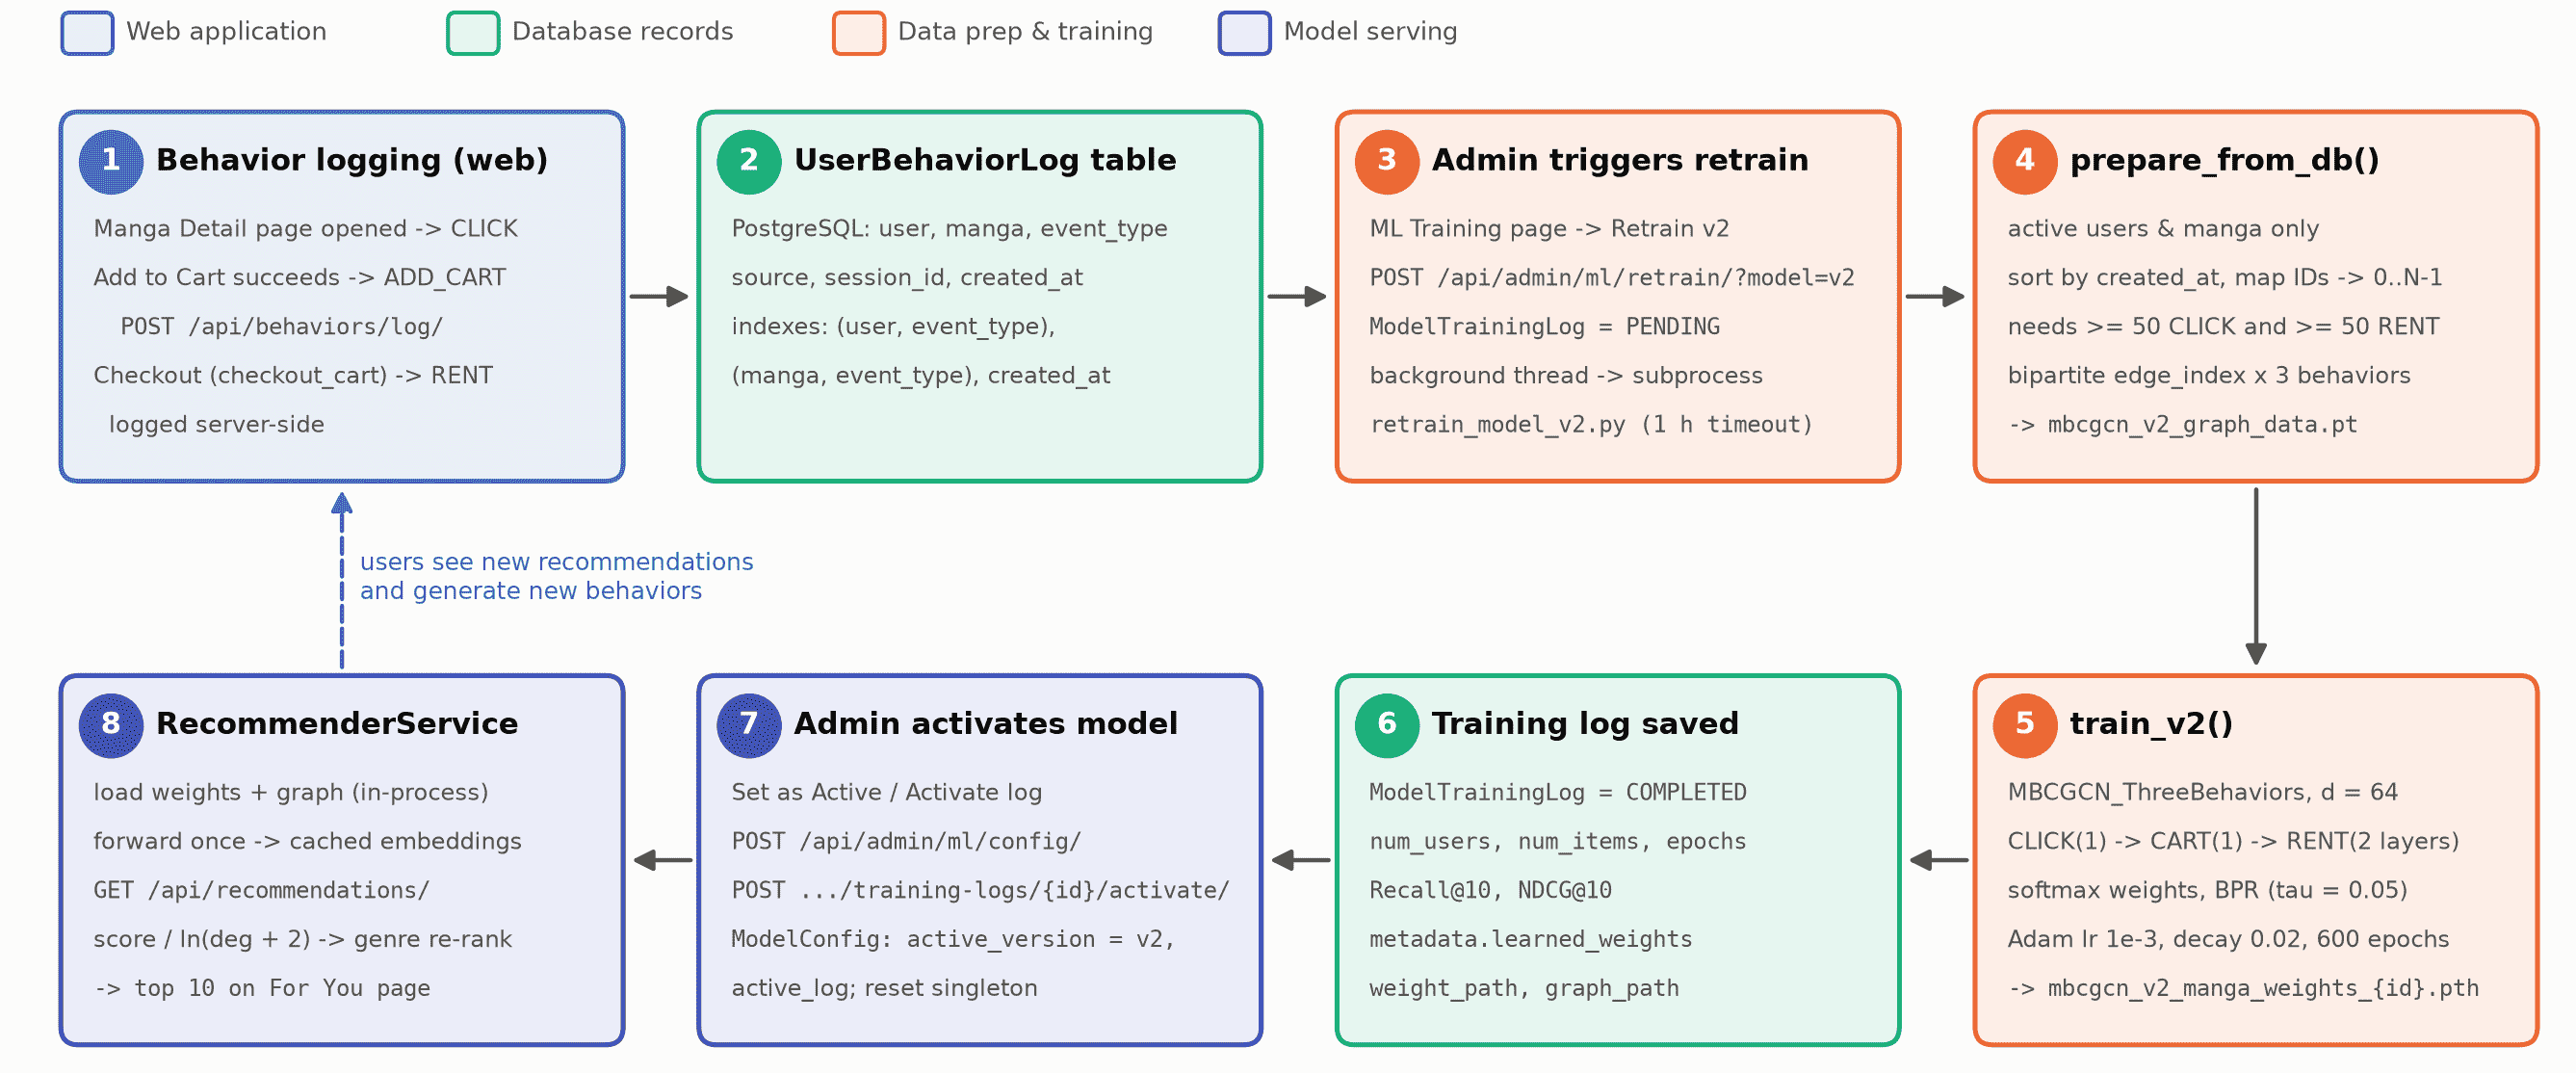
\includegraphics[width=0.9\textwidth]{images/fig_ch3_v2_data_pipeline.png}
\caption{ภาพรวมกระบวนการนำข้อมูลพฤติกรรมผู้ใช้จริงไปใช้ฝึกสอนโมเดลเวอร์ชัน 2}
\label{fig:ch4_114}
\end{figure}

\subsubsection{การโหลดและกรองข้อมูล}
ระบบจะโหลดข้อมูลจากไฟล์ Anime.csv และ User-AnimeReview.csv จากนั้นทำการกรองรายการโดยพิจารณาจากคอลัมน์ source ให้เหลือเฉพาะรายการที่มีต้นฉบับเป็นมังงะ เพื่อคัดรายการที่ไม่เกี่ยวข้อง เช่น อนิเมะต้นฉบับ ออกจากขอบเขตของระบบ ก่อนจะนำรหัสรายการที่ผ่านการกรองแล้วไปจับคู่กับข้อมูลปฏิสัมพันธ์ในไฟล์ User-AnimeReview.csv

\subsubsection{การแปลงดัชนี (ID Mapping)}
รหัสผู้ใช้ (user\_id) และรหัสรายการ (anime\_id) ซึ่งเป็นค่าไม่ต่อเนื่อง จะถูกแปลงเป็นดัชนีตัวเลขต่อเนื่องเริ่มจาก 0 (user\_idx, item\_idx) จากข้อมูลจริงพบว่ามีผู้ใช้ทั้งหมด 1,196,323 คน และรายการหนังสือการ์ตูนทั้งหมด 27,702 เรื่อง

\subsubsection{การแยกพฤติกรรมและแบ่งชุดข้อมูล}
ระบบแยกปฏิสัมพันธ์ออกเป็น 2 พฤติกรรม ได้แก่ พฤติกรรมการกดเข้าตะกร้า ซึ่งพิจารณาจากสถานะ ``Plan to Watch'' และพฤติกรรมการเช่า ซึ่งพิจารณาจากสถานะ ``Watching'' และ ``Completed'' โดยข้อมูลพฤติกรรมการเช่าจะถูกแบ่งออกเป็นชุดฝึกสอนและชุดทดสอบในสัดส่วน 80:20 (test\_size=0.20, random\_state=42) ด้วยฟังก์ชัน train\_test\_split จากไลบรารี scikit-learn เหตุผลที่ต้องแยกพฤติกรรมออกเป็นกราฟคนละชุดคือสถาปัตยกรรม MB-CGCN เรียนรู้แต่ละพฤติกรรมผ่านโครงข่ายกราฟ แยกกันก่อนนำผลลัพธ์มารวมกันในภายหลัง จึงจำเป็นต้องมีเอดจ์ของแต่ละพฤติกรรมแยกจากกันตั้งแต่ขั้นเตรียมข้อมูล โครงสร้างกราฟที่แยกตามพฤติกรรมแสดงดังภาพที่ \ref{fig:ch4_109}

สำหรับโมเดลเวอร์ชัน 2 (v2) ที่ใช้ห่วงโซ่ 3 ขั้น Click $\to$ Cart $\to$ Rent พฤติกรรม Click จะถูกสร้างจากข้อมูล UserBehaviorLog ที่บันทึกเหตุการณ์ CLICK เมื่อผู้ใช้คลิกดูรายละเอียดหนังสือ เนื่องจากข้อมูล MyAnimeList ไม่มีพฤติกรรมนี้ โมเดล v2 จึงฝึกจากข้อมูลพฤติกรรมจำลอง 1,000 ผู้ใช้กับหนังสือ 100 เรื่อง ซึ่งมีพฤติกรรมครบทั้งสามประเภท และแบ่งชุดฝึกกับชุดทดสอบในสัดส่วน 80:20 เช่นเดียวกับ v1 ตัวอย่างโครงสร้างข้อมูลจำลองที่ใช้ฝึก v2 แสดงดังตารางที่ \ref{tab:ch4_43}

\begin{table}[H]
\centering
\caption{ตัวอย่างข้อมูลพฤติกรรมจำลองที่ใช้ฝึกโมเดล v2}
\label{tab:ch4_43}
\small
\begin{tabular}{|c|c|c|l|}
\hline
\textbf{user\_id} & \textbf{manga\_id} & \textbf{event\_type} & \textbf{timestamp} \\ \hline
1 & 42 & CLICK & 2024-01-15 10:23:45 \\ \hline
1 & 42 & ADD\_TO\_CART & 2024-01-15 10:25:12 \\ \hline
1 & 42 & RENT & 2024-01-16 14:30:00 \\ \hline
1 & 87 & CLICK & 2024-01-18 09:15:33 \\ \hline
2 & 15 & CLICK & 2024-01-14 16:45:21 \\ \hline
2 & 15 & ADD\_TO\_CART & 2024-01-14 16:47:08 \\ \hline
2 & 23 & CLICK & 2024-01-17 11:20:45 \\ \hline
2 & 23 & RENT & 2024-01-19 13:10:22 \\ \hline
\end{tabular}
\end{table}

จากตัวอย่างในตารางที่ \ref{tab:ch4_43} จะเห็นว่าข้อมูลจำลองถูกออกแบบให้สะท้อนห่วงโซ่พฤติกรรมจริง โดยผู้ใช้ 1 คลิกดูหนังสือเรื่อง 42 ก่อน จากนั้นเพิ่มเข้าตะกร้า และทำการเช่าในภายหลัง ส่วนหนังสือเรื่อง 87 ผู้ใช้คลิกดูแต่ไม่ได้ทำขั้นตอนถัดไป และผู้ใช้ 2 มีพฤติกรรมคลิกดูหนังสือเรื่อง 23 แล้วเช่าโดยตรงโดยข้ามขั้นตอนตะกร้า ซึ่งสะท้อนพฤติกรรมการเช่าหน้าร้านที่ผู้ใช้อาจเลือกเช่าโดยตรงโดยไม่ผ่านระบบตะกร้า ข้อมูลจำลองทั้งหมดถูกสร้างให้มีลักษณะห่วงโซ่แบบนี้ครบทั้ง 1,000 ผู้ใช้ เพื่อทดสอบความสามารถของโมเดล v2 ในการเรียนรู้พฤติกรรมแบบ Cascading ก่อนที่ระบบจะสะสมข้อมูลจริงจากผู้ใช้งานจริงได้เพียงพอ

% TODO-IMG: img4_behavior_graph_structure.png -- วาดแผนภาพโครงสร้างกราฟแยกตามพฤติกรรม (edge_index_cart, edge_index_rent)
\begin{figure}[H]
\centering
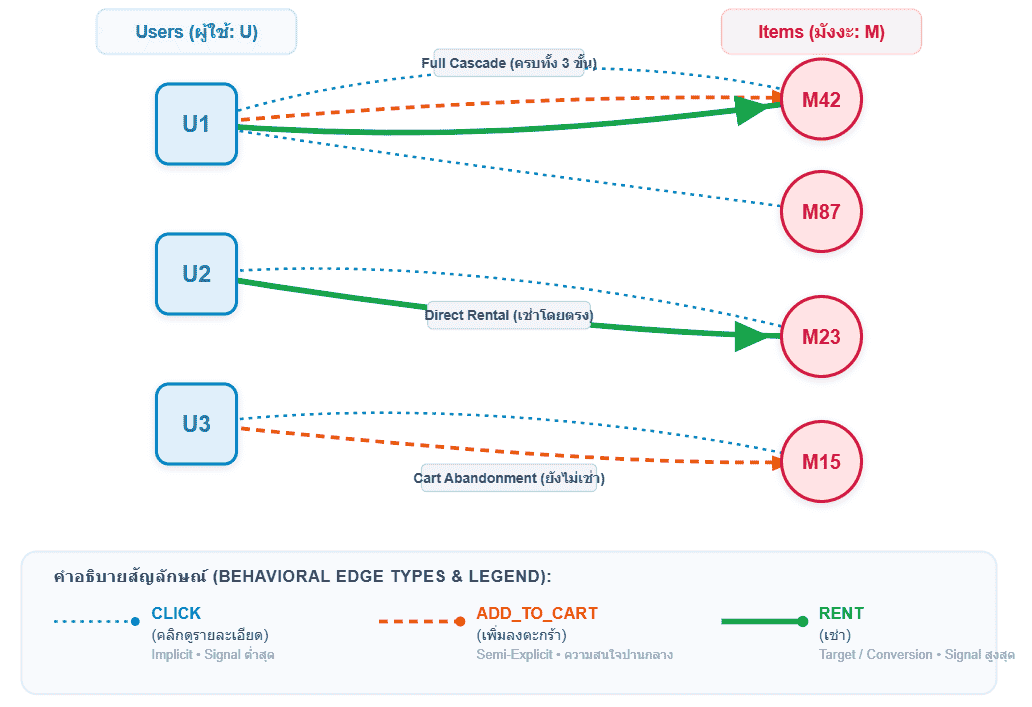
\includegraphics[width=0.8\textwidth]{images/img4_behavior_graph_structure.png}
\caption{โครงสร้างกราฟที่แยกตามพฤติกรรม (Cart และ Rent)}
\label{fig:ch4_109}
\end{figure}

ข้อมูลจะถูกนำเข้าในรูปแบบของเมทริกซ์ความสัมพันธ์ (Edge Index Tensors) ขนาด 2 × N โดยที่ N คือจำนวนการปฏิสัมพันธ์ แถวแรกจะเก็บดัชนีของผู้ใช้ และแถวที่สองจะเก็บดัชนีของหนังสือการ์ตูน จากการรันจริงได้ขนาดเทนเซอร์ดังนี้ กราฟการกดเข้าตะกร้ามีขนาด 2 × 4,897,807 กราฟการเช่าชุดฝึกสอนมีขนาด 2 × 8,298,820 และกราฟการเช่าชุดทดสอบมีขนาด 2 × 2,074,705 ทั้งหมดจะถูกบันทึกลงไฟล์ mbcgcn\_graph\_data.pt เพื่อนำไปใช้ในขั้นตอนฝึกสอนโมเดลต่อไป

\subsection{กระบวนการสร้างตัวแทนข้อมูล (Embedding Mechanism)}

กระบวนการ Embedding คือการแปลงข้อมูลผู้ใช้และหนังสือการ์ตูนให้อยู่ในรูปแบบของเวกเตอร์ตัวเลข เพื่อให้คอมพิวเตอร์สามารถเข้าใจและคำนวณความคล้ายคลึงกันได้

\subsubsection{สิ่งที่รับเข้าไป (Input)}
โมเดลจะรับค่า Index ID ของผู้ใช้ตั้งแต่ 0 ถึง $U$ (จำนวนผู้ใช้ทั้งหมด) และ Index ของหนังสือการ์ตูนตั้งแต่ 0 ถึง $I$ (จำนวนหนังสือทั้งหมด)

\subsubsection{กระบวนการ (Process)}
โมเดลจะใช้ฟังก์ชัน nn.Embedding ในการสร้างตารางค้นหา เพื่อแปลง Index แต่ละตัวให้กลายเป็น Latent Vector โดยกำหนดให้มีความยาว 64 มิติ 

\subsubsection{ผลลัพธ์ที่ได้ (Output)}
ในขั้นต้นนี้ จะได้เวกเตอร์ตัวแทนของผู้ใช้เริ่มต้น ($E_u^{(0)}$) และเวกเตอร์ตัวแทนของหนังสือเริ่มต้น ($E_i^{(0)}$) ที่พร้อมสำหรับการส่งเข้าสู่โครงข่ายกราฟ

\subsection{การออกแบบสถาปัตยกรรมโมเดล MB-CGCN}

สถาปัตยกรรมของโมเดล MB-CGCN ถูกออกแบบให้ทำงานแบบเรียงลำดับชั้น ตามแนวคิดห่วงโซ่พฤติกรรม โดยรองรับทั้งห่วงโซ่ 2 ขั้น (Cart $\rightarrow$ Rent สำหรับโมเดล v1) และห่วงโซ่ 3 ขั้น (Click $\rightarrow$ Cart $\rightarrow$ Rent สำหรับโมเดล v2) ในหัวข้อนี้จะอธิบายสถาปัตยกรรมโดยใช้โมเดล v1 ที่ครอบคลุม 2 บล็อกพฤติกรรม (Cart, Rent) เป็นหลัก ส่วนโมเดล v2 ใช้สถาปัตยกรรมเดียวกันแต่เพิ่มบล็อก Click เข้ามาขั้นแรก และเปลี่ยนน้ำหนักรวมพฤติกรรมจากค่าคงที่เป็นค่าที่ปรับได้ การประมวลผลแบ่งออกเป็น 4 ขั้นตอนหลัก ดังนี้

\subsubsection{การเรียนรู้พฤติกรรมเสริม (Auxiliary Behavior Modeling)}
นำเวกเตอร์เริ่มต้น ($E_u^{(0)}, E_i^{(0)}$) และกราฟตะกร้า ส่งเข้าสู่ชั้นการเรียนรู้กราฟ BehaviorGCN ซึ่งประกอบด้วยเลเยอร์ LightGCN จำนวน 1 ชั้น กระบวนการนี้จะทำให้โมเดลเรียนรู้ว่าผู้ใช้มีแนวโน้มสนใจหนังสือเรื่องใดบ้างในขั้นต้น ผลลัพธ์ที่ได้คือเวกเตอร์ของพฤติกรรมตะกร้า ($E_{cart}$)

\subsubsection{การคัดกรองและแปลงฟีเจอร์ (Feature Transformation)}
ระบบจะนำเวกเตอร์ $E_{cart}$ มาผ่านชั้น Linear Transformation (nn.Linear) เพื่อทำการคัดกรองสัญญาณรบกวนออก และสกัดเอาเฉพาะความรู้ที่เป็นประโยชน์ ส่งต่อไปเป็น ``ค่าเริ่มต้น'' ให้กับการเรียนรู้ในพฤติกรรมถัดไป

\subsubsection{การเรียนรู้พฤติกรรมเป้าหมาย (Target Behavior Modeling)}
นำเวกเตอร์ที่ผ่านการแปลงรูปแล้ว ส่งเข้าสู่ BehaviorGCN อีกชุดหนึ่ง จำนวน 1 ชั้นเช่นกัน พร้อมกับกราฟการเช่า เพื่อเรียนรู้พฤติกรรมขั้นสุดท้าย ผลลัพธ์ที่ได้คือเวกเตอร์ของการเช่า ($E_{rent}$)

\subsubsection{การรวมผลลัพธ์ (Embedding Aggregation)}
ในขั้นตอนสุดท้าย โมเดลจะนำเวกเตอร์ที่เรียนรู้ได้จากทั้งสองพฤติกรรมมารวมกันแบบถ่วงน้ำหนักคงที่ ในสัดส่วนพฤติกรรมตะกร้าร้อยละ 10 และพฤติกรรมการเช่าร้อยละ 90 ($0.1 \times E_{cart} + 0.9 \times E_{rent}$) ซึ่งเป็นสัดส่วนที่ได้จากการปรับจูนไฮเปอร์พารามิเตอร์ (Hyperparameter Tuning) ดังรายละเอียดในหัวข้อผลการทดสอบ เพื่อสร้างเป็น ``เวกเตอร์ผลลัพธ์สุดท้าย'' ของผู้ใช้และหนังสือการ์ตูนที่สมบูรณ์ที่สุด

\subsection{การทำนายและข้อมูลส่งออก (Prediction and Output Data)}

เมื่อระบบต้องการแนะนำหนังสือการ์ตูนให้กับผู้ใช้งาน จะมีกระบวนการคำนวณผลลัพธ์ดังนี้

\subsubsection{การคำนวณคะแนน}
ระบบจะนำเวกเตอร์ผลลัพธ์สุดท้ายของผู้ใช้เป้าหมาย ไปทำ Dot Product (การคูณเชิงสเกลาร์) กับเวกเตอร์ผลลัพธ์สุดท้ายของหนังสือการ์ตูนทุกเรื่องในระบบ ซึ่งจะได้ออกมาเป็น ``คะแนนความน่าจะเป็น'' ดังตัวอย่างโค้ดในภาพที่ \ref{fig:ch4_104}

% TODO-IMG: แคปจาก backend/rentals/recommender.py:330-340
\begin{figure}[H]
\centering
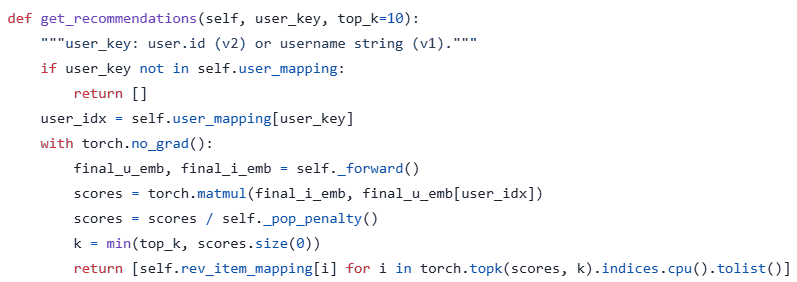
\includegraphics[width=0.85\textwidth]{images/code4_recommender_scoring.png}
\caption{ขั้นตอนการคำนวณคะแนนแนะนำในฟังก์ชัน get\_recommendations}
\label{fig:ch4_104}
\end{figure}
ภาพที่ \ref{fig:ch4_104} แสดงส่วนหนึ่งของฟังก์ชัน get\_recommendations ในไฟล์ recommender.py ซึ่งคำนวณคะแนนด้วย Dot Product ระหว่างเวกเตอร์ผู้ใช้และเวกเตอร์หนังสือการ์ตูนทุกเรื่อง ก่อนนำไปจัดเรียงลำดับเพื่อเลือก Top-K ผลลัพธ์

\subsubsection{ข้อมูลส่งออก}
โมเดลจะทำการจัดเรียงลำดับคะแนนจากมากไปน้อย โดยในกรณีที่คำนวณคะแนนจากเวกเตอร์เฉลี่ยของหนังสือที่ผู้ใช้เคยมีปฏิสัมพันธ์ด้วย ระบบจะคัดกรอง (Masking) หนังสือกลุ่มนั้นออกจากผลลัพธ์โดยปรับคะแนนเป็นลบอนันต์ ($-\infty$) ก่อนเรียงลำดับ จากนั้นจึงส่งออกผลลัพธ์ในรูปแบบของรายการดัชนีหนังสือการ์ตูนที่ได้คะแนนสูงสุด 10 อันดับแรก กลับไปยังระบบเพื่อแสดงผลให้ผู้ใช้เห็นต่อไป ดัชนีเหล่านี้มีความแตกต่างกันระหว่างโมเดลรุ่นที่ 1 และรุ่นที่ 2 กล่าวคือ โมเดลรุ่นที่ 1 อ้างอิงผู้ใช้ด้วยรหัส mbrs\_id หรือชื่อผู้ใช้จากชุดข้อมูล MyAnimeList โดยตรง ในขณะที่โมเดลรุ่นที่ 2 อ้างอิงผู้ใช้ด้วยรหัส id ของผู้ใช้ในระบบ Django เอง เนื่องจากฝึกสอนจากข้อมูลพฤติกรรมที่เกิดขึ้นจริงในเว็บแอปพลิเคชัน จึงต้องมีการแปลงดัชนีให้สอดคล้องกับโมเดลที่ถูกเลือกใช้งานในขณะนั้นก่อนส่งคำขอ

ฝั่งเซิร์ฟเวอร์จะรับผลลัพธ์ดัชนีดังกล่าวมาประกอบกับข้อมูลหนังสือการ์ตูนแต่ละเรื่อง ก่อนส่งกลับเป็น JSON ผ่าน API endpoint GET /api/recommendations/ ให้ส่วนหน้าเว็บแสดงผล ดังตัวอย่างใน \ref{fig:ch4_110}

% TODO-IMG: code4_recommendation_json.png -- capture ผลลัพธ์ JSON จริงจากการเรียก GET /api/recommendations/ (เช่นจาก Postman หรือ DevTools Network tab) ให้เห็นฟิลด์ recommendations, popular_fill, has_preferences
\begin{figure}[H]
\centering
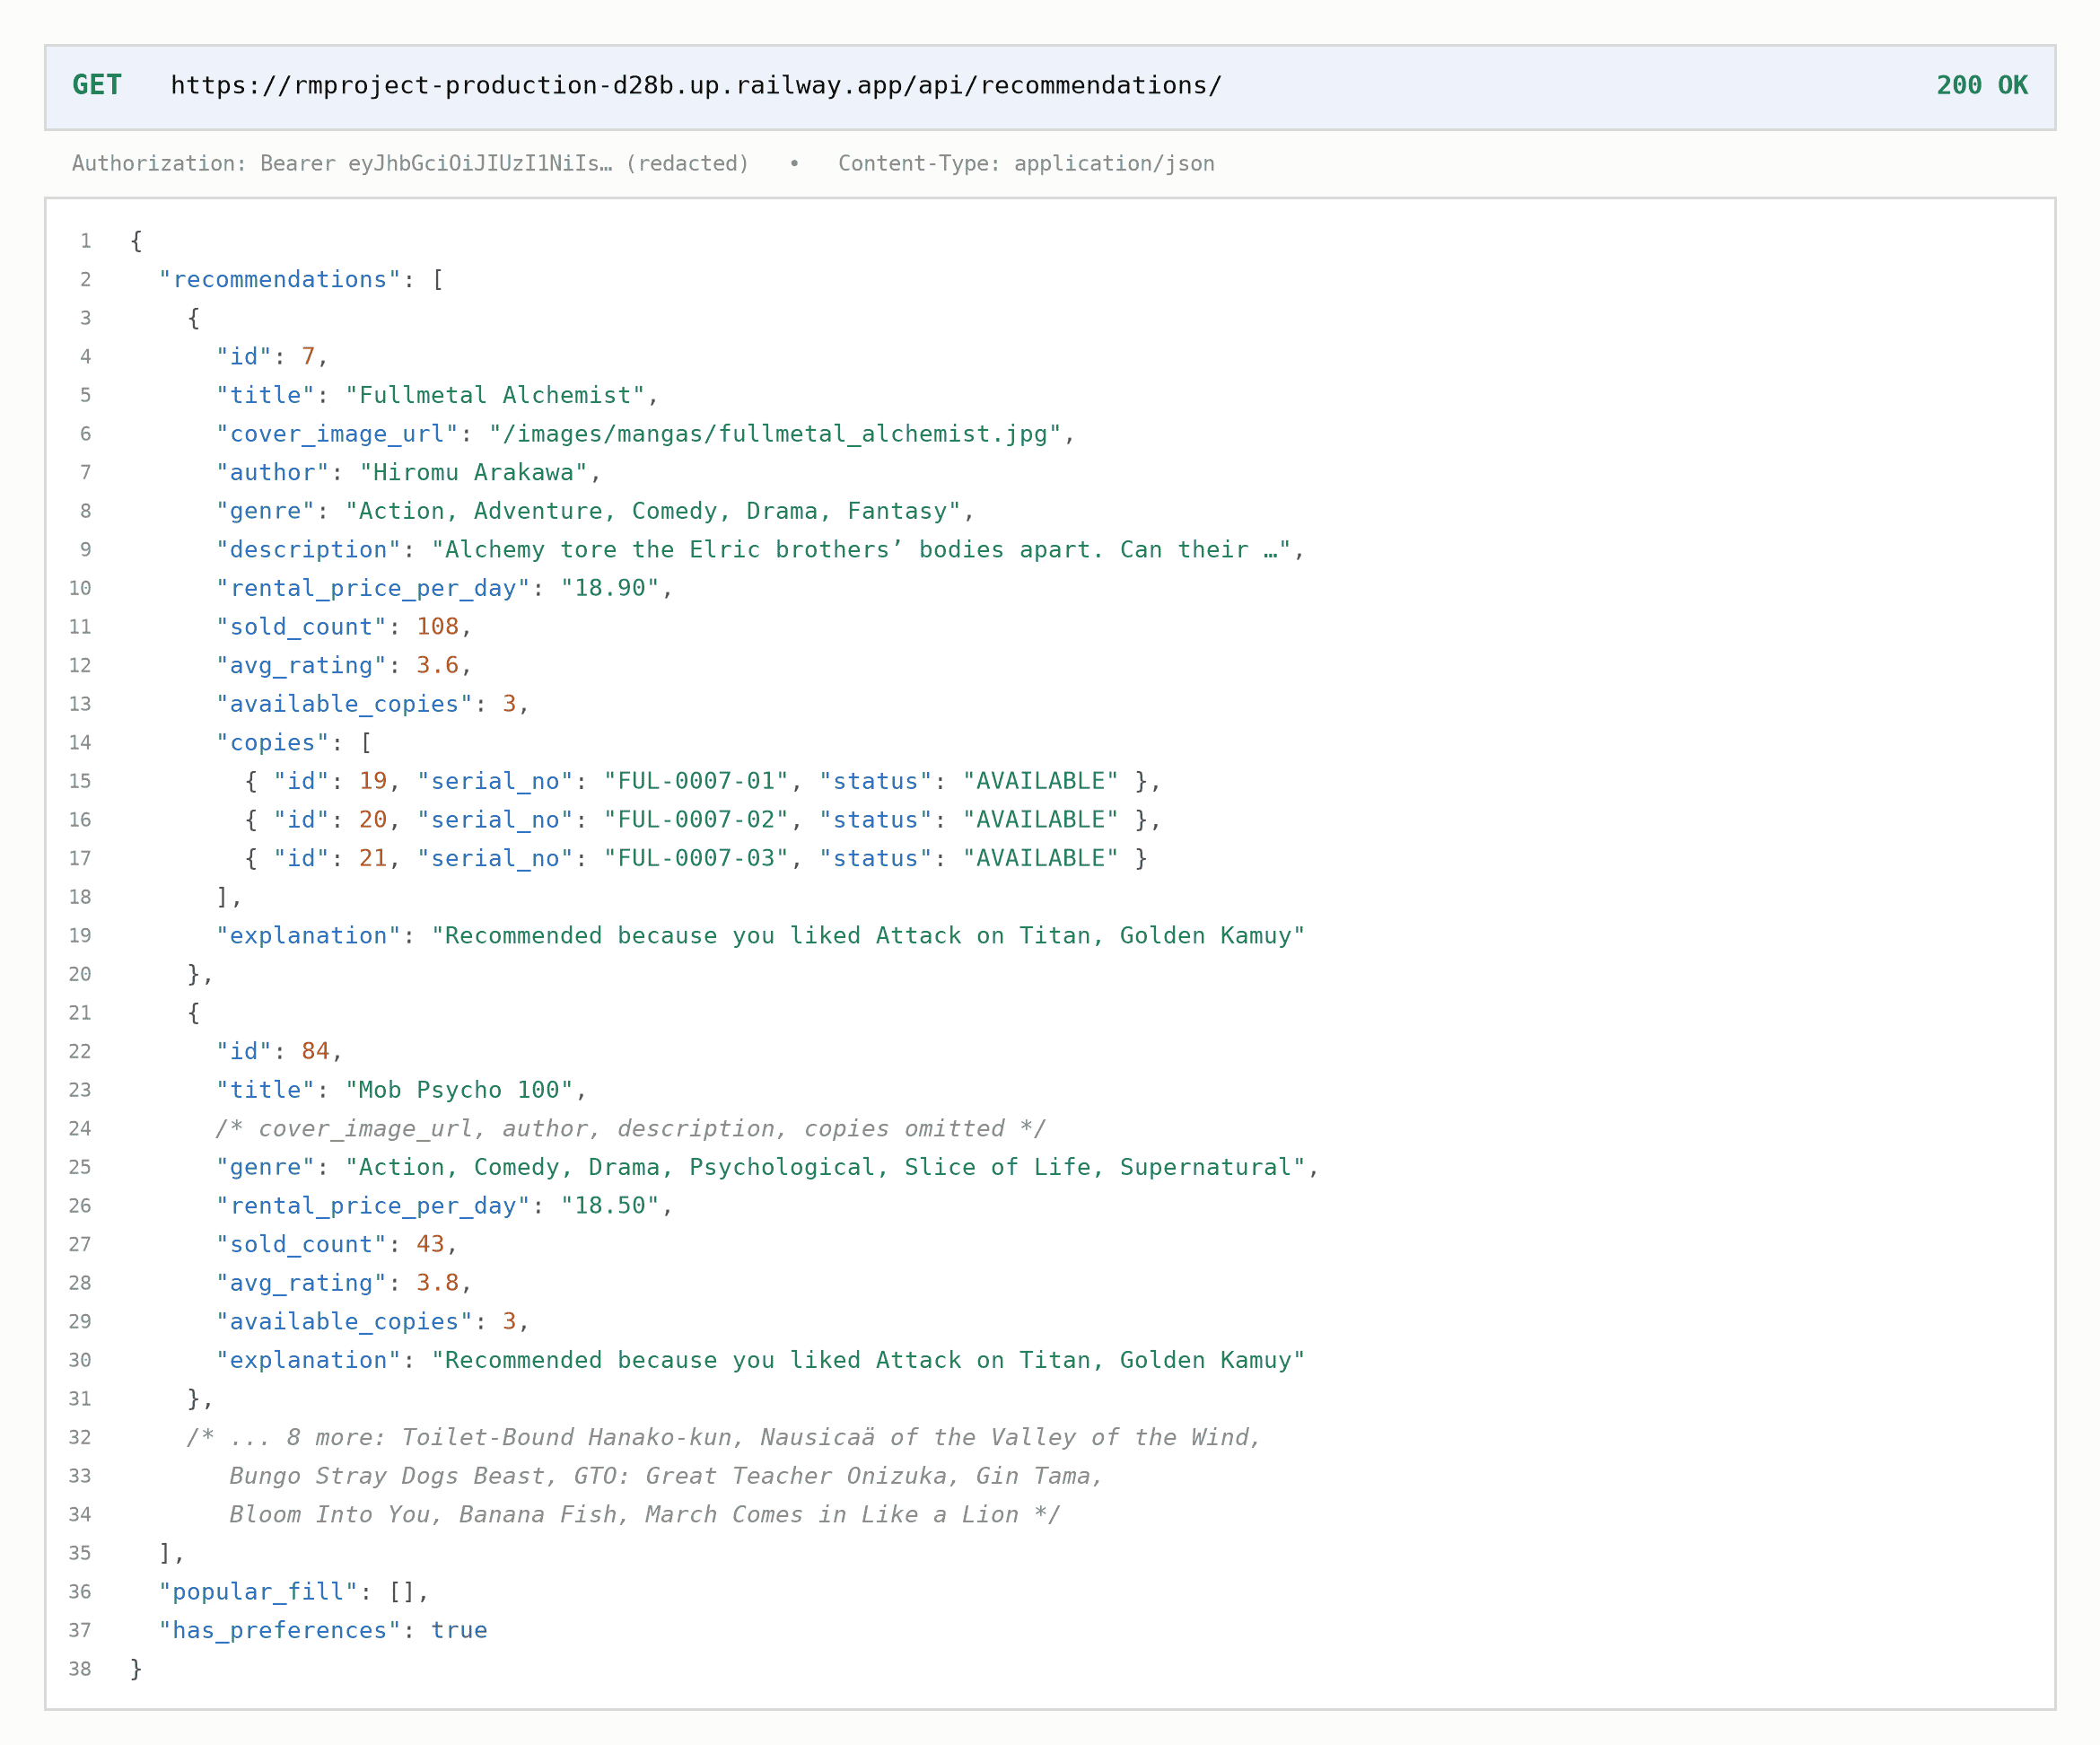
\includegraphics[width=0.9\textwidth]{images/code4_recommendation_json.png}
\caption{ตัวอย่างผลลัพธ์ JSON ที่ได้จาก API GET /api/recommendations/}
\label{fig:ch4_110}
\end{figure}

ภาพที่ \ref{fig:ch4_110} แสดงโครงสร้าง JSON ของผลลัพธ์ ซึ่งในกรณีที่ระบบสามารถคำนวณคะแนนจากโมเดลได้ จะส่งคืนฟิลด์ recommendations ซึ่งก็คือรายการหนังสือที่โมเดลแนะนำ พร้อมคำอธิบายเหตุผลในฟิลด์ explanation ของแต่ละเรื่อง จะนำฟิลด์ popular\_fill ที่เป็นรายการหนังสือเติมเต็มจากความนิยม กรณีผลลัพธ์จากโมเดลมีไม่ครบ 10 เรื่อง และฟิลด์ has\_preferences ที่เป็นค่า Boonlean ระบุว่าผู้ใช้มีข้อมูล UserPreference หรือไม่ ส่วนกรณีที่ไม่สามารถคำนวณผลลัพธ์จากโมเดลได้เลยและผู้ใช้ไม่มีประวัติการเช่า ระบบจะคืนค่าฟิลด์ recommendations เป็นรายการหนังสือใหม่และหนังสือที่ได้รับความนิยมสูงสุดแทน พร้อมฟิลด์ explanation\_type ที่มีค่าเป็น popular และฟิลด์ explanation อธิบายเหตุผลของรายการทั้งหมด

\subsection{การแนะนำสำหรับผู้ใช้ที่ไม่มีประวัติในชุดข้อมูลฝึกสอน}

ระบบแนะนำต้องรองรับกรณีที่ผู้ใช้งานจริงในเว็บแอปพลิเคชันไม่มีประวัติอยู่ในชุดข้อมูล MyAnimeList ที่ใช้ฝึกสอนโมเดล ซึ่งแบ่งออกเป็น 2 กรณีหลัก ดังนี้

\subsubsection{ตัวตนจำลองจากประวัติการเช่าในระบบ}
กรณีผู้ใช้ไม่มีดัชนีในกราฟที่ใช้ฝึกสอน แต่มีประวัติการเช่าหนังสือการ์ตูนในระบบจริงแล้ว ฟังก์ชัน get\_item\_based\_recommendations จะดึงเวกเตอร์ผลลัพธ์สุดท้ายของหนังสือที่ผู้ใช้เคยเช่า แล้วคำนวณค่าเฉลี่ย ของเวกเตอร์เหล่านั้นขึ้นมาเป็นเวกเตอร์ตัวตนจำลอง (Pseudo User Embedding) แทนเวกเตอร์ผู้ใช้ที่โมเดลไม่เคยเรียนรู้ จากนั้นจึงนำเวกเตอร์ตัวตนจำลองนี้ไปทำ Dot Product กับเวกเตอร์หนังสือทุกเรื่องเช่นเดียวกับกรณีผู้ใช้ปกติ

\subsubsection{การแก้ปัญหา Cold-Start จากข้อมูลความสนใจเริ่มต้น}
กรณีผู้ใช้สมัครสมาชิกใหม่และยังไม่มีประวัติการเช่าใด ๆ ระบบจะให้ผู้ใช้เลือกหนังสือการ์ตูนที่สนใจจำนวน 4 เรื่องในขั้นตอนเริ่มต้นใช้งาน (Onboarding) หรือสามารถปรับใหม่ได้ภายหลัง โดยบันทึกไว้ในตาราง UserPreference ฟังก์ชัน get\_recommendations\_with\_explanations จะใช้รหัสหนังสือที่เลือกไว้สร้างเวกเตอร์ตัวตนจำลองด้วยวิธี Mean Pooling แบบเดียวกับกรณีประวัติการเช่า เพื่อให้ระบบสามารถแนะนำหนังสือที่คล้ายคลึงกันได้ทันทีโดยไม่ต้องรอข้อมูลพฤติกรรมเพิ่มเติม

\subsubsection{การจัดอันดับใหม่ตามประเภทหนังสือที่ชอบ}
เมื่อผู้ใช้มีข้อมูลความสนใจ ระบบจะนำประเภทหนังสือ ของหนังสือที่ผู้ใช้เลือกไว้มาคำนวณน้ำหนักความสนใจต่อแต่ละประเภท โดยประเภทที่ปรากฏซ้ำหลายครั้งจะได้น้ำหนักสูงกว่าประเภทที่ปรากฏเพียงครั้งเดียว จากนั้นฟังก์ชัน genre\_rerank จะปรับคะแนนของหนังสือแต่ละเรื่องในผลลัพธ์เบื้องต้นแบบคูณ (Multiplicative Bonus) ตามสัดส่วนการทับซ้อนของประเภทหนังสือกับความสนใจของผู้ใช้ รวมถึงสามารถแทรกหนังสือที่ตรงกับประเภทที่ผู้ใช้ชอบแต่โมเดลไม่ได้จัดอยู่ในลำดับต้น ๆ เข้ามาในกลุ่มที่พิจารณาใหม่ได้ด้วย เพื่อให้ผลการแนะนำสอดคล้องกับความสนใจเชิงประเภทของผู้ใช้มากขึ้น ผลลัพธ์สุดท้ายที่ผ่านการคำนวณคะแนน การคัดกรอง Cold-Start และการจัดอันดับใหม่ตามประเภทแล้ว จะถูกแสดงให้ผู้ใช้เห็นที่หน้า For You ดังภาพที่ \ref{fig:ch4_113}

\begin{figure}[H]
\centering
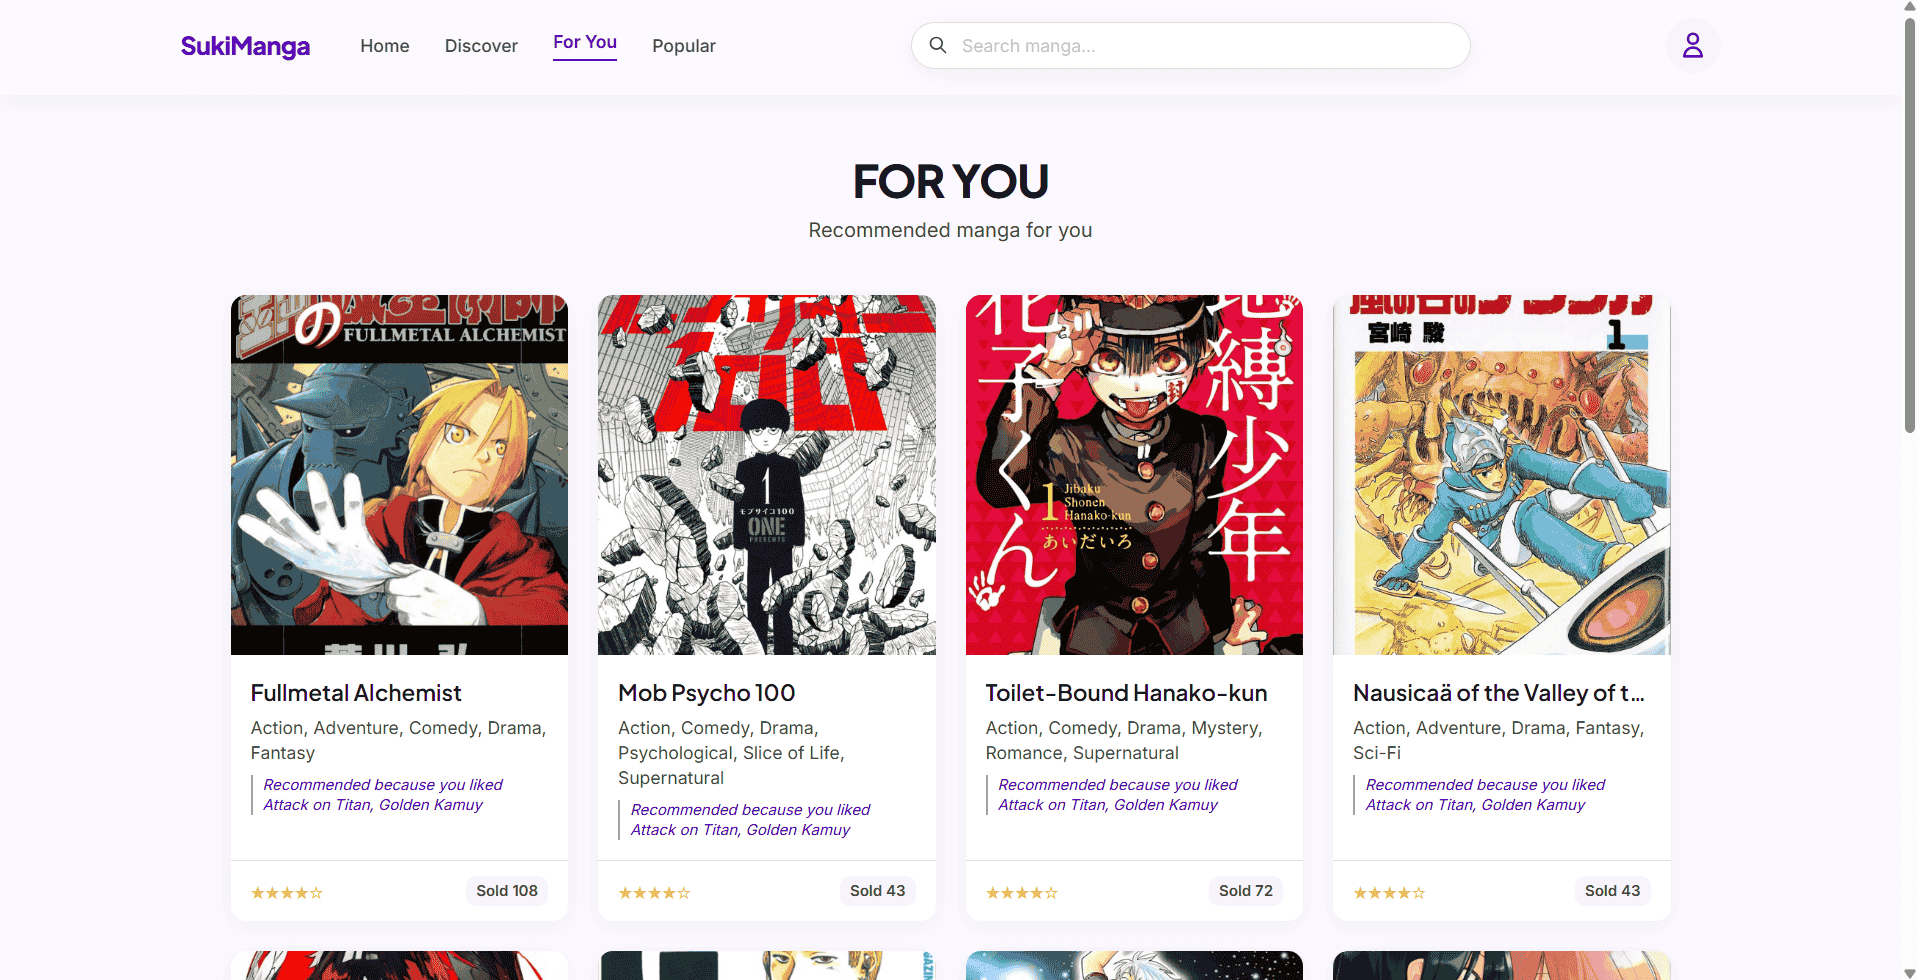
\includegraphics[width=0.85\textwidth]{images/foryoupage.png}
\caption{หน้า For You แสดงรายการหนังสือการ์ตูนที่ระบบแนะนำให้ผู้ใช้}
\label{fig:ch4_113}
\end{figure}

\subsection{การตั้งค่าและพารามิเตอร์ในการฝึกสอนโมเดล (Training Configuration)}

ก่อนเข้าสู่ขั้นตอนฝึกสอน โมเดลทุกตัวที่นำมาทดลอง ทั้งโมเดลฐานและโมเดล MBRS ถูกฝึกสอนภายใต้เงื่อนไขและพารามิเตอร์ชุดเดียวกันเพื่อให้สามารถเปรียบเทียบผลลัพธ์ได้อย่างยุติธรรม โดยพัฒนาและรันการทดลองบนแพลตฟอร์ม Google Colab ด้วยเฟรมเวิร์ก PyTorch ร่วมกับไลบรารี PyTorch Geometric ใช้เลเยอร์ LGConv ในการทำ Graph Convolution พารามิเตอร์สำคัญ 2 ตัวที่ปรากฏในตาราง ได้แก่ BPR Loss (Bayesian Personalized Ranking Loss) ซึ่งเป็นฟังก์ชันสูญเสียที่ออกแบบมาสำหรับงานจัดอันดับโดยเฉพาะ โดยฝึกให้โมเดลให้คะแนนคู่ผู้ใช้ \- หนังสือที่มีปฏิสัมพันธ์จริง (Positive) สูงกว่าคู่ที่ไม่มีปฏิสัมพันธ์ (Negative) และ Negative Sampling ซึ่งเป็นกระบวนการสุ่มเลือกหนังสือที่ผู้ใช้ยังไม่มีปฏิสัมพันธ์มาเป็นตัวอย่าง Negative สำหรับคำนวณ BPR Loss ในแต่ละรอบ รายละเอียดพารามิเตอร์ทั้งหมดแสดงดังตารางที่ \ref{tab:ch4_36}

\begin{table}[H]
\centering
\caption{พารามิเตอร์ที่ใช้ในการฝึกสอนโมเดล v1 และ v2}
\label{tab:ch4_36}
\small
\renewcommand{\arraystretch}{1.4}  % ระยะบนล่าง (ปกติ = 1)
\setlength{\tabcolsep}{8pt}        % ระยะซ้ายขวา (ปกติ = 6pt)
\newcolumntype{L}[1]{>{\raggedright\arraybackslash}p{#1}}
\begin{tabular}{|L{4.2cm}|L{4.2cm}|L{4.2cm}|}
\hline
\textbf{พารามิเตอร์} & \textbf{v1 (Cart $\rightarrow$ Rent)} & \textbf{v2 (Click $\rightarrow$ Cart $\rightarrow$ Rent)} \\ \hline
ชุดข้อมูล & MyAnimeList \newline (700,000+ ผู้ใช้) & ข้อมูลจำลอง \newline (1,000 ผู้ใช้ $\times$ 100 หนังสือ) \\ \hline
จำนวนพฤติกรรม & 2 ชั้น (Cart, Rent) & 3 ชั้น (Click, Cart, Rent) \\ \hline
มิติเวกเตอร์ตัวแทน (embed\_dim) & 64 & 64 \\ \hline
จำนวนเลเยอร์ GCN & 1 ชั้นต่อพฤติกรรม & Click: 1 ชั้น, Cart: 1 ชั้น, Rent: 2 ชั้น \\ \hline
น้ำหนักพฤติกรรม & สัดส่วนคงที่ (10:90) & Adaptive Weights \newline (เรียนรู้อัตโนมัติ) \\ \hline
Loss Function & BPR Loss, $\tau = 0.05$ & BPR Loss \\ \hline
Negative Sampling & Popularity-based \newline (ยกกำลัง 0.75) & Popularity-based \newline (ยกกำลัง 0.75) \\ \hline
Optimizer & Adam, LR = 0.001 & Adam, LR = 0.001 \\ \hline
LR Scheduler & StepLR \newline (ลดครึ่งหนึ่งทุก 100 Epoch) & ไม่ใช้ \\ \hline
L2 Regularization ($\lambda$) & 0.02 (คำนวณใน Loss) & 0.01 \newline (weight\_decay ใน Optimizer) \\ \hline
Batch/Sample Size & 400,000 คู่ปฏิสัมพันธ์ต่อ Epoch & 512 คู่ปฏิสัมพันธ์ต่อ Batch \\ \hline
จำนวน Epochs & 600 & 600 \\ \hline
Evaluation Interval & ทุก 20--50 Epoch & ทุก 50 Epoch \\ \hline
วิธีวัดผล & สุ่ม 1,000 ผู้ใช้จากชุดทดสอบ & ใช้ผู้ใช้ทั้งหมดในชุดทดสอบ \\ \hline
\end{tabular}
\end{table}

เนื่องจากขั้นตอนการวัดผลระหว่างการฝึกสอนโมเดล v1 ใช้วิธีสุ่มตัวอย่างผู้ใช้จากชุดทดสอบเพียง 1,000 คนในแต่ละรอบ (ไม่ใช่การประเมินด้วยผู้ใช้ทั้งหมด เพื่อความรวดเร็ว) ค่า Recall และ NDCG ที่วัดได้ในแต่ละ Epoch จึงมีความผันผวน (Fluctuation) ได้บ้างตามธรรมชาติของการสุ่ม ส่วนโมเดล v2 ใช้ผู้ใช้ทั้งหมดในชุดทดสอบเพราะกราฟมีขนาดเล็กกว่า ผลลัพธ์โดยละเอียดของแต่ละโมเดลแสดงไว้ในหัวข้อผลการทดสอบถัดไป

ตารางที่ \ref{tab:ch4_36} แสดงพารามิเตอร์ที่ใช้ฝึกสอนทั้งสองเวอร์ชัน ความแตกต่างหลักระหว่าง v1 และ v2 คือ v2 มีพฤติกรรมเพิ่มเป็น 3 ชั้น ใช้น้ำหนักพฤติกรรมแบบปรับได้อัตโนมัติ แทนสัดส่วนคงที่ เพิ่มจำนวนเลเยอร์ GCN ของพฤติกรรม Rent เป็น 2 ชั้น และใช้ข้อมูลจำลองขนาดเล็ก (1,000 ผู้ใช้ × 100 หนังสือ) เพื่อทดสอบกลไกก่อนมีข้อมูลจริงเพียงพอ นอกจากนี้ v2 ใช้ weight\_decay ของ Optimizer Adam โดยตรงแทนการคำนวณ L2 Regularization เข้าไปในค่า Loss และไม่ใช้ LR Scheduler

\subsection{การพัฒนาโมเดลเวอร์ชัน 2 และน้ำหนักพฤติกรรมแบบปรับได้}

หลังจากพัฒนาโมเดล MB-CGCN เวอร์ชันแรก (v1) ที่ใช้พฤติกรรมเช่าสองลำดับคือ Cart และ Rent แล้ว ทีมผู้พัฒนาได้ขยายโมเดลเป็นเวอร์ชันที่ 2 (v2) ซึ่งเพิ่มพฤติกรรม Click เข้ามาเป็นพฤติกรรมเสริมลำดับแรก ทำให้สายโซ่พฤติกรรมเป็น Click $\to$ Cart $\to$ Rent เพื่อให้โมเดลสามารถเรียนรู้สัญญาณความสนใจของผู้ใช้ได้ตั้งแต่ขั้นตอนการดูรายละเอียดหนังสือ ก่อนจะมีการหยิบลงตะกร้าหรือทำการเช่าจริง

ความแตกต่างสำคัญอีกประการของโมเดล v2 คือการเปลี่ยนจากน้ำหนักรวมพฤติกรรมแบบคงที่ ในโมเดล v1 ไปเป็นน้ำหนักที่ปรับค่าได้ระหว่างการฝึกสอน โดยกำหนดค่าเริ่มต้นของน้ำหนักทั้งสามพฤติกรรมเป็นพารามิเตอร์ที่เรียนรู้ได้ แล้วผ่านฟังก์ชัน Softmax เพื่อให้ผลรวมน้ำหนักเท่ากับ 1 เสมอ วิธีนี้ทำให้โมเดลสามารถเรียนรู้ได้เองว่าพฤติกรรมใดควรมีอิทธิพลต่อผลการทำนายมากหรือน้อยกว่ากัน แทนการกำหนดสัดส่วนตายตัวโดยผู้พัฒนา ระบบรองรับการสลับใช้งานระหว่างโมเดล v1 และ v2 ผ่านการตั้งค่า ModelConfig ซึ่งผู้ดูแลระบบสามารถเลือกเวอร์ชันที่ต้องการให้บริการจริงได้ โครงสร้างคลาสของโมเดล v2 แสดงดังภาพที่ \ref{fig:ch4_102}

% TODO-IMG: แคปจาก ml_model/models/mbcgcn_v2.py:48-87
\begin{figure}[H]
\centering
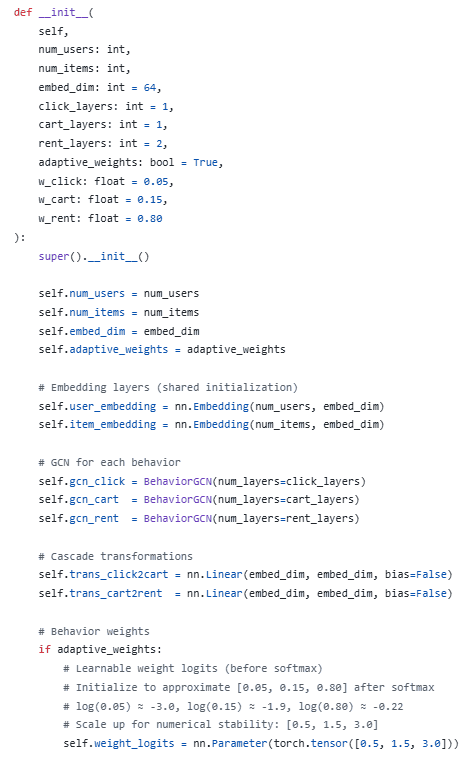
\includegraphics[width=0.85\textwidth]{images/code4_mbcgcn_class.png}
\caption{โครงสร้างคลาส MBCGCN\_ThreeBehaviors ในไฟล์ mbcgcn\_v2.py}
\label{fig:ch4_102}
\end{figure}
ภาพที่ \ref{fig:ch4_102} แสดงส่วนประกอบหลักของคลาส MBCGCN\_ThreeBehaviors ได้แก่ Embedding ของผู้ใช้และหนังสือการ์ตูน ชั้น BehaviorGCN ของแต่ละพฤติกรรม และพารามิเตอร์ weight\_logits ที่ใช้เป็นน้ำหนักเรียนรู้ได้สำหรับการรวมผลลัพธ์แบบ Adaptive Weights

ในด้านฟังก์ชันสูญเสีย โมเดลทั้ง v1 และ v2 ใช้ BPR Loss แบบเดียวกัน โดยคำนวณจากผลต่างคะแนนระหว่างคู่หนังสือที่ผู้ใช้มีปฏิสัมพันธ์จริง (Positive) และคู่ที่สุ่มมา (Negative) ดังแสดงในภาพที่ \ref{fig:ch4_103}

% TODO-IMG: แคปจาก ml_model/scripts/train_v2.py:20-34
\begin{figure}[H]
\centering
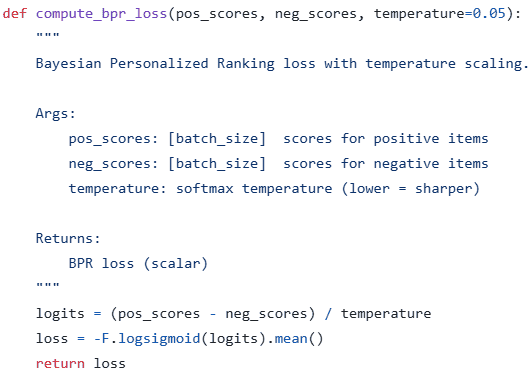
\includegraphics[width=0.85\textwidth]{images/code4_bpr_loss.png}
\caption{ฟังก์ชันคำนวณ BPR Loss ในสคริปต์ train\_v2.py}
\label{fig:ch4_103}
\end{figure}
ภาพที่ \ref{fig:ch4_103} แสดงฟังก์ชันคำนวณ BPR Loss ซึ่งนำผลต่างคะแนนของคู่ Positive และ Negative มาผ่าน Log-Sigmoid แล้วใส่เครื่องหมายลบเพื่อให้เป็นค่าที่ต้องลดให้น้อยที่สุดระหว่างการฝึกสอน

\subsection{การทดลอง A/B Testing}

ระบบมีโครงสร้างสำหรับการทดลองแบบ A/B Testing เพื่อเปรียบเทียบประสิทธิภาพของโมเดลหรือกลยุทธ์การแนะนำหลายรูปแบบกับผู้ใช้จริง โดยคลาส ABTestManager ทำหน้าที่สุ่มกำหนดกลุ่มทดลอง ให้แต่ละผู้ใช้ตามสัดส่วนน้ำหนักที่กำหนดไว้ และบันทึกการกำหนดกลุ่มของผู้ใช้แต่ละคนให้คงที่ เพื่อให้ผู้ใช้คนเดียวกันอยู่ในกลุ่มทดลองเดิมเสมอในการเข้าใช้งานครั้งต่อ ๆ ไป นอกจากนี้ยังมีฟังก์ชันสำหรับบันทึกเหตุการณ์ เช่น การเห็นรายการแนะนำ การคลิก การเพิ่มลงตะกร้า และการเช่าสำเร็จ เพื่อนำไปคำนวณตัวชี้วัดอย่าง Click-Through Rate (CTR) และ Conversion Rate ของแต่ละกลุ่มทดลอง ผู้ดูแลระบบสามารถจัดการกลุ่มทดลองและดูผลตัวชี้วัดเหล่านี้ได้ผ่านหน้าแดชบอร์ดผู้ดูแลระบบ ขั้นตอนการสุ่มกำหนดกลุ่มทดลองแสดงดังภาพที่ \ref{fig:ch4_105}

% TODO-IMG: แคปจาก backend/rentals/ab_testing.py:13-44
\begin{figure}[H]
\centering
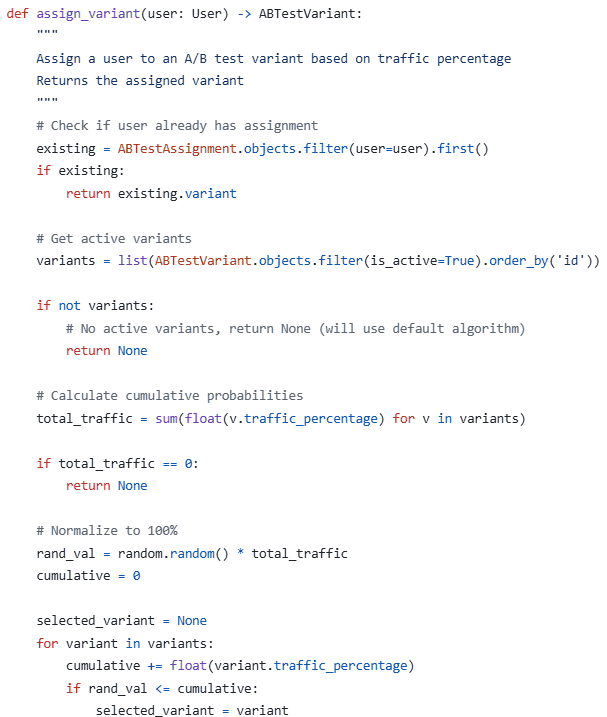
\includegraphics[width=0.85\textwidth]{images/code4_ab_assign.png}
\caption{ฟังก์ชัน assign\_variant สำหรับกำหนดกลุ่มทดลอง A/B Testing}
\label{fig:ch4_105}
\end{figure}
ภาพที่ \ref{fig:ch4_105} แสดงฟังก์ชัน assign\_variant ของคลาส ABTestManager ซึ่งตรวจสอบว่าผู้ใช้มีกลุ่มทดลองที่กำหนดไว้แล้วหรือไม่ หากยังไม่มีจะคำนวณสัดส่วนสะสม (Cumulative Traffic Percentage) ของแต่ละกลุ่มทดลอง แล้วสุ่มค่าเพื่อเลือกกลุ่มทดลองตามสัดส่วนนั้น 

ระบบ A/B Testing ในโครงงานนี้มีโครงสร้างพื้นฐานครบถ้วน ได้แก่ ตารางฐานข้อมูล คลาส ABTestManager และหน้าจอผู้ดูแลระบบสำหรับติดตามผล อย่างไรก็ตาม ฟังก์ชัน assign\_variant และ track\_event ยังไม่ถูกเรียกใช้จาก RecommendationView ผู้ใช้ทุกคนจึงยังได้รับอัลกอริทึมเดียวกัน และตัวชี้วัดในหน้าผู้ดูแลระบบแสดงค่า 0 เสมอ เพื่อให้การทดสอบ A/B ทำงานได้จริง ต้องเชื่อมโค้ดในส่วน RecommendationView ให้เรียก assign\_variant เพื่อแบ่งกลุ่มผู้ใช้ และบันทึกพฤติกรรมด้วย track\_event ซึ่งจะช่วยวัดประสิทธิภาพของอัลกอริทึมต่าง ๆ กับผู้ใช้จริงได้

% TODO: ตรวจสอบ ไม่พบการเรียกใช้ ABTestManager.assign\_variant หรือ get\_user\_variant จากฝั่ง RecommendationView หรือ endpoint แนะนำหนังสือใด ๆ ในซอร์สโค้ดปัจจุบัน จึงยังไม่สามารถยืนยันได้ว่ามีการนำผลการแบ่งกลุ่มไปใช้สลับอัลกอริทึมการแนะนำที่ให้บริการจริงกับผู้ใช้ปลายทางหรือไม่
อย่างไรก็ตาม ในปัจจุบันการแนะนำหนังสือที่ให้บริการจริงผ่าน /api/recommendations/ ยังใช้โมเดลเดียวตามที่กำหนดไว้ใน ModelConfig สำหรับผู้ใช้ทุกคนเหมือนกัน โครงสร้าง A/B Testing ที่พัฒนาไว้จึงอยู่ในลักษณะเครื่องมือพร้อมใช้สำหรับการทดลองและเก็บข้อมูลตัวชี้วัดในอนาคต 

\subsection{การฝึกสอนโมเดลใหม่โดยผู้ดูแลระบบ}

เพื่อให้ระบบสามารถปรับปรุงโมเดลแนะนำให้ทันกับข้อมูลพฤติกรรมผู้ใช้ที่เพิ่มขึ้นได้โดยไม่ต้องเข้าถึงเซิร์ฟเวอร์โดยตรง ผู้พัฒนาได้จัดทำกลไกการฝึกสอนโมเดลใหม่ที่สั่งงานผ่านหน้าแดชบอร์ดผู้ดูแลระบบ โดยเมื่อผู้ดูแลระบบเลือกเวอร์ชันโมเดลที่ต้องการฝึกสอนใหม่ ระบบจะเรียกใช้สคริปต์ฝึกสอน เป็น Subprocess แยกจาก process หลักของเว็บเซิร์ฟเวอร์ เพื่อไม่ให้การฝึกสอนที่ใช้เวลานานไปปิดกั้นการให้บริการผู้ใช้งานทั่วไป ระหว่างการฝึกสอนผู้ดูแลระบบสามารถตรวจสอบสถานะความคืบหน้าได้ และเมื่อฝึกสอนเสร็จสิ้นผลลัพธ์จะถูกบันทึกเป็นประวัติการฝึกสอน โดยผู้ดูแลระบบต้องเลือกยืนยัน ประวัติการฝึกสอนที่ต้องการนำไปใช้งานจริงด้วยตนเองอีกครั้งหนึ่ง การฝึกสอนใหม่ทั้งหมดจึงเกิดขึ้นจากการสั่งงานของผู้ดูแลระบบเท่านั้น ไม่มีการฝึกสอนซ้ำแบบอัตโนมัติตามรอบเวลา

กล่าวโดยสรุป ความเชื่อมโยงระหว่างระบบแนะนำกับการใช้งานจริงของเว็บแอปพลิเคชันเกิดขึ้นเป็นวงจรต่อเนื่อง 3 ขั้นตอน ได้แก่ ขั้นตอนที่ 1 การบันทึกพฤติกรรม (Behavior Logging) ซึ่งทุกครั้งที่ผู้ใช้คลิกดูรายละเอียดหนังสือ เพิ่มลงตะกร้า หรือเช่าหนังสือสำเร็จ ระบบจะบันทึกเหตุการณ์เหล่านี้ลงตาราง UserBehavior ขั้นตอนที่ 2 การฝึกสอนโมเดลใหม่โดยผู้ดูแลระบบ (Admin-Triggered Retraining) ซึ่งผู้ดูแลระบบจะนำข้อมูลพฤติกรรมที่สะสมไว้มาสั่งฝึกสอนโมเดลรุ่นที่ 2 ใหม่ผ่านหน้าแดชบอร์ดตามที่อธิบายไว้ข้างต้น เพื่อให้โมเดลเรียนรู้รูปแบบความสนใจที่เปลี่ยนแปลงไปของผู้ใช้งานจริง และขั้นตอนที่ 3 การเลือกใช้งานโมเดลเวอร์ชันที่ฝึกสอนเสร็จ (Model Activation) ซึ่งผู้ดูแลระบบจะตรวจสอบผลการประเมินของประวัติการฝึกสอนแต่ละครั้ง แล้วเลือกยืนยัน (Activate) เวอร์ชันที่ต้องการนำไปให้บริการจริง จากนั้นค่า ModelConfig จะถูกปรับให้ชี้ไปยังไฟล์น้ำหนักโมเดลเวอร์ชันดังกล่าว ทำให้คำขอแนะนำหนังสือครั้งต่อไปทุกคำขอใช้โมเดลเวอร์ชันใหม่นี้ทันที วงจรทั้ง 3 ขั้นตอนนี้ทำให้ระบบแนะนำสามารถปรับปรุงให้สอดคล้องกับพฤติกรรมผู้ใช้จริงได้อย่างต่อเนื่อง แม้ว่าในปัจจุบันทุกขั้นตอนยังต้องอาศัยการสั่งงานของผู้ดูแลระบบ ไม่มีการฝึกสอนและสลับเวอร์ชันโมเดลแบบอัตโนมัติ

\subsection{Scheduled Background Job}

นอกจากกลไกด้านโมเดลแนะนำแล้ว ระบบยังมีงานประมวลผลตามรอบเวลา (Scheduled Job) ที่ทำงานอยู่ใน process เดียวกับเว็บเซิร์ฟเวอร์ Django โดยใช้ไลบรารี APScheduler ตั้งเวลาให้ทำงานทุกเที่ยงคืน เพื่อตรวจสอบรายการเช่าที่มีสถานะค้างชำระ และเกินกำหนดส่งคืนเป็นเวลานานกว่า 90 วัน หากพบรายการดังกล่าว ระบบจะปรับสถานะของรายการเช่าและสำเนาหนังสือที่เกี่ยวข้องเป็นสูญหายโดยอัตโนมัติ เพื่อให้ข้อมูลสถานะหนังสือในระบบสอดคล้องกับความเป็นจริงโดยไม่ต้องให้ผู้ดูแลระบบตรวจสอบด้วยตนเองทุกวัน

\section{การทดสอบระบบ}

การทดสอบระบบในส่วนนี้แบ่งออกเป็น 2 ส่วน ได้แก่ การทดสอบการทำงานของระบบแนะนำในลักษณะกรณีทดสอบ (Test Case) ที่ตรวจสอบว่าแต่ละสถานการณ์การใช้งานให้ผลลัพธ์ตามที่คาดหวังหรือไม่ และการประเมินประสิทธิภาพของโมเดลด้วยตัวชี้วัดเชิงปริมาณที่นิยมใช้ในงานวิจัยระบบแนะนำ ได้แก่ Recall@K และ NDCG@K

Recall@K คือสัดส่วนของหนังสือที่ผู้ใช้มีปฏิสัมพันธ์จริงในชุดทดสอบ ที่โมเดลสามารถจัดอยู่ใน K อันดับแรกของรายการแนะนำได้ ค่ายิ่งสูงแสดงว่าโมเดลค้นหาหนังสือที่ผู้ใช้สนใจจริงได้ครอบคลุมมากขึ้น ส่วน NDCG@K (Normalized Discounted Cumulative Gain at K) คือตัวชี้วัดที่พิจารณาทั้งว่าหนังสือที่ถูกต้องปรากฏอยู่ใน K อันดับแรกหรือไม่ และตำแหน่งที่ปรากฏ โดยให้น้ำหนักกับผลลัพธ์ที่อยู่ในอันดับต้น ๆ มากกว่าอันดับท้าย ๆ ค่ายิ่งสูงแสดงว่าโมเดลไม่เพียงหาหนังสือที่ถูกต้องเจอ แต่ยังจัดลำดับให้อยู่ใกล้อันดับต้นมากขึ้นด้วย งานวิจัยนี้เลือกวัดผลที่ K=10 และ K = 20 เนื่องจาก K = 10 สอดคล้องกับจำนวนรายการแนะนำสูงสุดที่ระบบแสดงจริงต่อผู้ใช้ 1 ครั้ง (Top - 10) ในขณะที่ K = 20 ช่วยสะท้อนความสามารถของโมเดลในระดับที่กว้างกว่าหน้าจอแสดงผลจริง ทำให้เห็นแนวโน้มของโมเดลได้ชัดเจนขึ้น

การประเมินผลทั้งหมดใช้ข้อมูลพฤติกรรมการเช่า ที่แบ่งออกเป็นชุดฝึกสอนและชุดทดสอบในสัดส่วน 80:20 ตามที่อธิบายไว้ในหัวข้อการเตรียมข้อมูล โดยโมเดลจะไม่เคยเห็นข้อมูลในชุดทดสอบระหว่างการฝึกสอนเลย เพื่อให้ค่า Recall@K และ NDCG@K ที่วัดได้สะท้อนความสามารถในการแนะนำหนังสือให้กับสถานการณ์ที่โมเดลไม่เคยพบมาก่อนอย่างแท้จริง และเนื่องจากชุดทดสอบมีผู้ใช้จำนวนมาก การคำนวณตัวชี้วัดในทุก Epoch จึงสุ่มตัวอย่างผู้ใช้มาเพียง 1,000 คนต่อครั้ง เพื่อให้การฝึกสอนและประเมินผลเสร็จภายในเวลาที่เหมาะสม ซึ่งเป็นข้อจำกัดที่ควรพิจารณาควบคู่กับผลลัพธ์ที่ได้ กล่าวคือค่าตัวชี้วัดที่รายงานเป็นค่าประมาณจากกลุ่มตัวอย่าง มิใช่ค่าที่คำนวณจากผู้ใช้ทุกคนในชุดทดสอบ

\subsection{Test Case พร้อมผล Pass/Fail}

ผลการทดสอบโมเดลระบบแนะนำ แสดงดังตารางที่ \ref{tab:ch4_33}

\begin{longtable}{|c|p{3cm}|p{3.5cm}|p{3.5cm}|c|}
\caption{Test Case} \label{tab:ch4_33} \\
\hline
\textbf{รหัสทดสอบ} & \textbf{กรณีทดสอบ} & \textbf{ผลลัพธ์ที่คาดหวัง} & \textbf{ผลลัพธ์จริง} & \textbf{สถานะ} \\ \hline
\endfirsthead
\caption[]{Test Case (ต่อ)} \\
\hline
\textbf{รหัสทดสอบ} & \textbf{กรณีทดสอบ} & \textbf{ผลลัพธ์ที่คาดหวัง} & \textbf{ผลลัพธ์จริง} & \textbf{สถานะ} \\ \hline
\endhead
TC-MBRS-01 & เข้าสู่ระบบด้วยผู้ใช้ที่มีประวัติการฝึกสอนในโมเดล & ระบบดึงเวกเตอร์ของผู้ใช้ มาคำนวณและคืนค่าหนังสือการ์ตูนแนะนำ 10 อันดับแรกได้อย่างแม่นยำ & ระบบคืนค่าหนังสือการ์ตูน 10 เรื่อง อิงจากความน่าจะเป็นสูงสุด & Pass \\ \hline
TC-MBRS-02 & ผู้ใช้ไม่มีใน Dataset แต่ระบบ Local DB มีประวัติว่าเคยเช่าหนังสือ & ระบบสร้าง ''ตัวตนจำลอง'' จากประวัติการเช่าเดิม และคืนค่าหนังสือที่มีความคล้ายคลึงกัน 10 ลำดับ & ระบบคืนค่าหนังสือการ์ตูน 10 เรื่อง อิงจากความน่าจะเป็นสูงสุด & Pass \\ \hline
TC-MBRS-03 & ผู้ใช้เพิ่งสมัครสมาชิกและเลือกหนังสือการ์ตูนที่สนใจไว้ & ระบบสร้างโปรไฟล์ความสนใจเริ่มต้นจากหนังสือที่ผู้ใช้เลือก และแนะนำหนังสือที่คล้ายคลึงกัน 10 เรื่องทันที (แก้ปัญหา Cold-Start) & ระบบคืนค่าหนังสือการ์ตูน 10 เรื่องที่สัมพันธ์กับความสนใจที่ผู้ใช้เลือก & Pass \\ \hline
TC-MBRS-04 & ตรวจสอบผลลัพธ์การแนะนำของผู้ใช้ที่ไม่มีประวัติในชุดข้อมูลฝึกสอนแต่มีประวัติการเช่าหนังสือการ์ตูนในระบบ & หนังสือการ์ตูนที่ผู้ใช้เคยทำการเช่าไปแล้ว จะต้องถูกปรับคะแนนเป็นลบอนันต์ และไม่แสดงซ้ำในผลลัพธ์ & ผลลัพธ์ 10 อันดับแรกไม่มีหนังสือการ์ตูนที่ผู้ใช้เคยเช่าปรากฏอยู่ & Pass \\ \hline
TC-MBRS-05 & เรียกใช้งาน Endpoint GET /api/recommendations/ พร้อมส่ง JWT Token & ระบบคืนค่า JSON Response ที่มีสถานะ 200 OK พร้อมข้อมูลรายละเอียดหนังสือครบถ้วน & ระบบคืนค่ารูปแบบ JSON ที่ถูกต้อง สามารถนำไปแสดงผลได้ & Pass \\ \hline
TC-MBRS-06 & ผู้ใช้เพิ่มหนังสือลงในตะกร้าแล้วทำการเช่าสำเร็จ จากนั้นเรียกดูส่วน "แนะนำสำหรับคุณ" ในการเข้าใช้งานครั้งถัดไป & สำหรับผู้ใช้ที่สร้างคำแนะนำจากตัวตนจำลอง (Pseudo User) ผลการแนะนำจะเปลี่ยนไปตามประวัติการเช่าล่าสุดที่นำไปคำนวณเวกเตอร์เฉลี่ยใหม่ & ผลการแนะนำเปลี่ยนแปลงตามประวัติการเช่าที่อัปเดตแล้ว & Pass \\ \hline
TC-MBRS-07 & ผู้ใช้คลิกอ่านเนื้อหาของหนังสือเล่มใดเล่มหนึ่ง (บันทึกผ่าน /api/behaviors/log/) แล้วเรียกดูส่วน "แนะนำสำหรับคุณ" ทันที & ข้อมูลการคลิกถูกบันทึกไว้สำหรับใช้ฝึกสอนโมเดลเวอร์ชัน 2 ในอนาคต แต่ยังไม่มีผลต่อผลการแนะนำที่แสดงในทันที เนื่องจากโมเดลที่ให้บริการอยู่ไม่ได้คำนวณผลใหม่จากพฤติกรรม Click แบบเรียลไทม์ & ผลการแนะนำยังคงเดิม ไม่เปลี่ยนแปลงตามการคลิกล่าสุดในทันที & Pass \\ \hline
\end{longtable}

\subsection{ผลการทดสอบ}

ในการทดลอง ได้ทำการฝึกสอนโมเดลทั้งหมด 4 รุ่นภายใต้พารามิเตอร์ชุดเดียวกัน (ตารางที่ \ref{tab:ch4_36}) เป็นระยะเวลา 600 Epoch เท่ากันทุกโมเดล ได้แก่ (1) Baseline MF เรียนรู้จากพฤติกรรมการเช่าล้วนๆ โดยไม่ผ่านกราฟ (2) Baseline LightGCN เรียนรู้จากพฤติกรรมการเช่าเพียงพฤติกรรมเดียวแต่ผ่านการทำ Graph Convolution (3) MB-CGCN (น้ำหนักเรียนรู้เอง) ซึ่งเป็นการทดลองปรับจูนไฮเปอร์พารามิเตอร์เพื่อหาสัดส่วนอิทธิพลระหว่าง Cart และ Rent ที่เหมาะสม และ (4) MBRS (MB-CGCN สัดส่วนคงที่ Cart 10\% : Rent 90\%) ซึ่งเป็นโมเดลที่นำเสนอในโครงงานนี้ ผลการเปรียบเทียบภาพรวมแสดงดังภาพที่ \ref{fig:ch4_58}

\begin{figure}[H]
\centering
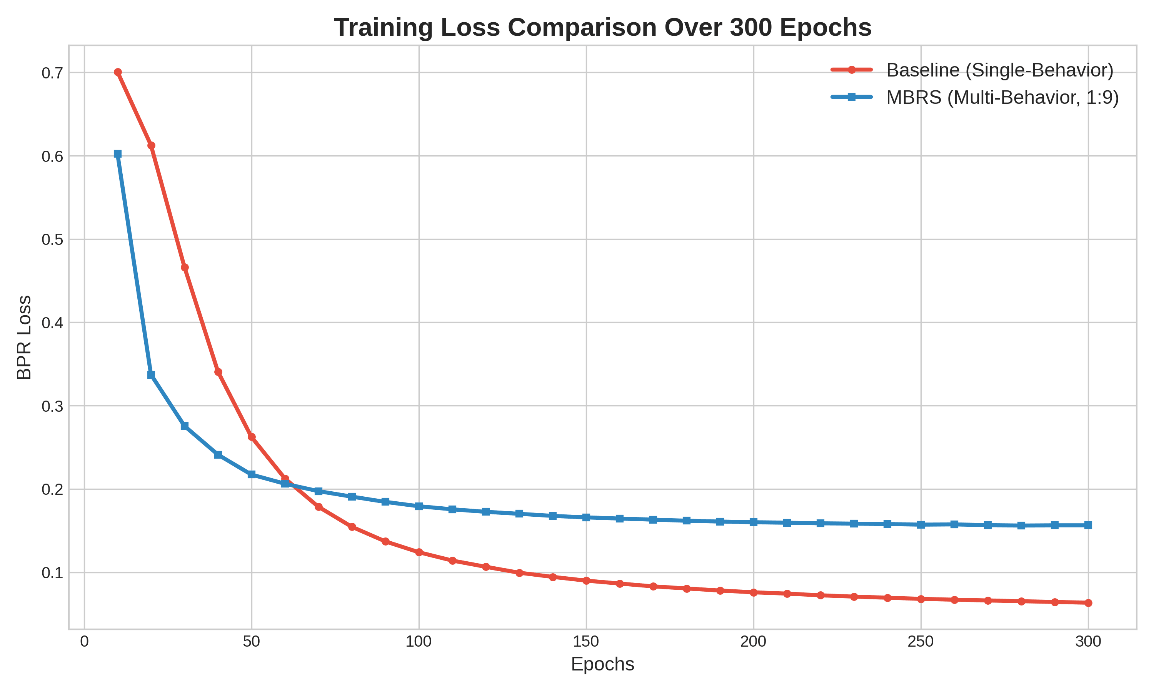
\includegraphics[width=0.85\textwidth]{images/4image58.png}
\caption{กราฟเปรียบเทียบผลการทดสอบระหว่างโมเดลฐานและโมเดล MBRS}
\label{fig:ch4_58}
\end{figure}

\subsubsection{ผลการทดสอบโมเดลฐานที่ 1: Matrix Factorization (Baseline MF)}

โมเดล MF เป็นโมเดลพื้นฐานที่สุด ใช้เวกเตอร์ตัวแทนของผู้ใช้และหนังสือการ์ตูนโดยตรงโดยไม่ผ่านชั้นกราฟใดๆ เพื่อใช้เป็นเส้นฐาน (Baseline) เทียบว่าการเพิ่ม Graph Convolution และการรวมพฤติกรรมหลายแบบช่วยเพิ่มประสิทธิภาพได้จริงหรือไม่ ผลลัพธ์ที่จุดวัดผลต่างๆ แสดงดังตารางที่ \ref{tab:ch4_37}

\begin{table}[H]
\centering
\caption{ประสิทธิภาพของโมเดล Baseline MF ณ ช่วงเวลาต่างๆ}
\label{tab:ch4_37}
\small
\begin{tabular}{|c|c|c|c|c|c|}
\hline
\textbf{Epoch} & \textbf{Loss} & \textbf{Recall@10} & \textbf{NDCG@10} & \textbf{Recall@20} & \textbf{NDCG@20} \\ \hline
100 & 0.1859 & 0.0202 & 0.0170 & 0.0334 & 0.0209 \\ \hline
200 & 0.1345 & 0.0370 & 0.0311 & 0.0559 & 0.0369 \\ \hline
300 & 0.1208 & 0.0339 & 0.0295 & 0.0550 & 0.0356 \\ \hline
400 & 0.1128 & 0.0386 & 0.0348 & 0.0660 & 0.0421 \\ \hline
500 & 0.1091 & 0.0451 & 0.0361 & 0.0654 & 0.0420 \\ \hline
600 & 0.1079 & 0.0378 & 0.0336 & 0.0641 & 0.0412 \\ \hline
\end{tabular}
\end{table}

\begin{figure}[H]
\centering
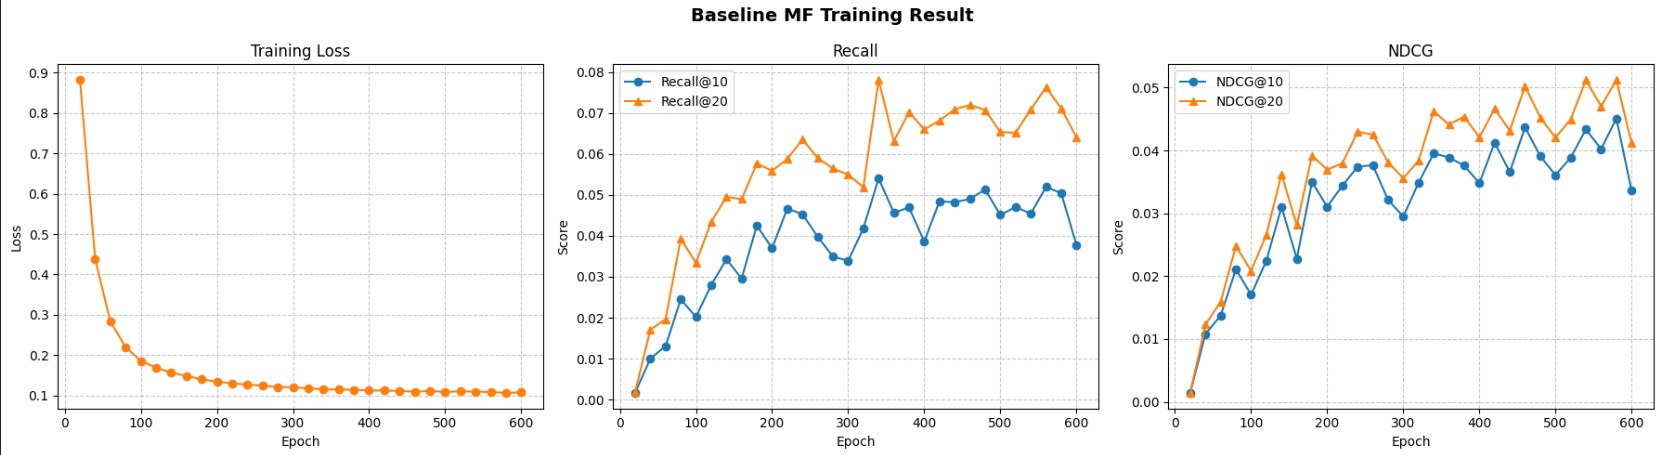
\includegraphics[width=\textwidth]{images/4image59.jpg}
\caption{กราฟผลการฝึกสอนของโมเดล Baseline MF (Loss, Recall, NDCG)}
\label{fig:ch4_59}
\end{figure}

จากตารางที่ \ref{tab:ch4_37} พบว่าค่า Loss ของโมเดล MF ลดลงอย่างต่อเนื่องจาก 0.8816 (Epoch 20) ลงมาจนถึง 0.1079 ในช่วงท้าย สะท้อนว่าโมเดลเรียนรู้ค่าพารามิเตอร์ได้อย่างมีเสถียรภาพ อย่างไรก็ตาม ค่า Recall@20 และ NDCG@20 มีแนวโน้มผันผวนขึ้นลงในช่วง Epoch ที่ 300 เป็นต้นไป โดย Recall@20 แกว่งตัวในช่วง 0.055--0.078 และ NDCG@20 แกว่งตัวในช่วง 0.036--0.051 ซึ่งเป็นผลจากการที่โมเดลไม่มีกลไก Graph Convolution ช่วยกระจายสัญญาณระหว่างผู้ใช้ที่มีพฤติกรรมใกล้เคียงกัน ทำให้ความสามารถในการจัดอันดับไม่พัฒนาขึ้นอย่างสม่ำเสมอ กราฟผลการฝึกสอนของโมเดล Baseline MF แสดงในภาพที่ \ref{fig:ch4_59}

\subsubsection{ผลการทดสอบโมเดลฐานที่ 2: Single-Behavior GCN (Baseline LightGCN)}

โมเดล LightGCN เป็นโมเดลฐานที่ใช้ Graph Convolution เช่นเดียวกับ MBRS แต่เรียนรู้จากพฤติกรรมการเช่า เพียงพฤติกรรมเดียว โดยไม่มีการนำพฤติกรรมการกดเข้าตะกร้า มาเป็นสัญญาณเสริม ใช้เพื่อวัดว่าการเพิ่มพฤติกรรมหลายแบบแบบ Cascading ช่วยเพิ่มประสิทธิภาพเมื่อเทียบกับ GCN พฤติกรรมเดียวหรือไม่ ผลลัพธ์แสดงดังตารางที่ \ref{tab:ch4_38}

\begin{table}[H]
\centering
\caption{ประสิทธิภาพของโมเดล Baseline LightGCN ณ ช่วงเวลาต่างๆ}
\label{tab:ch4_38}
\small
\begin{tabular}{|c|c|c|c|c|c|}
\hline
\textbf{Epoch} & \textbf{Loss} & \textbf{Recall@10} & \textbf{NDCG@10} & \textbf{Recall@20} & \textbf{NDCG@20} \\ \hline
100 & 0.1841 & 0.0293 & 0.0243 & 0.0433 & 0.0283 \\ \hline
200 & 0.1335 & 0.0215 & 0.0219 & 0.0335 & 0.0247 \\ \hline
300 & 0.1196 & 0.0394 & 0.0328 & 0.0535 & 0.0375 \\ \hline
400 & 0.1125 & 0.0532 & 0.0422 & 0.0760 & 0.0489 \\ \hline
500 & 0.1099 & 0.0401 & 0.0332 & 0.0614 & 0.0392 \\ \hline
600 & 0.1082 & 0.0444 & 0.0426 & 0.0619 & 0.0470 \\ \hline
\end{tabular}
\end{table}

\begin{figure}[H]
\centering
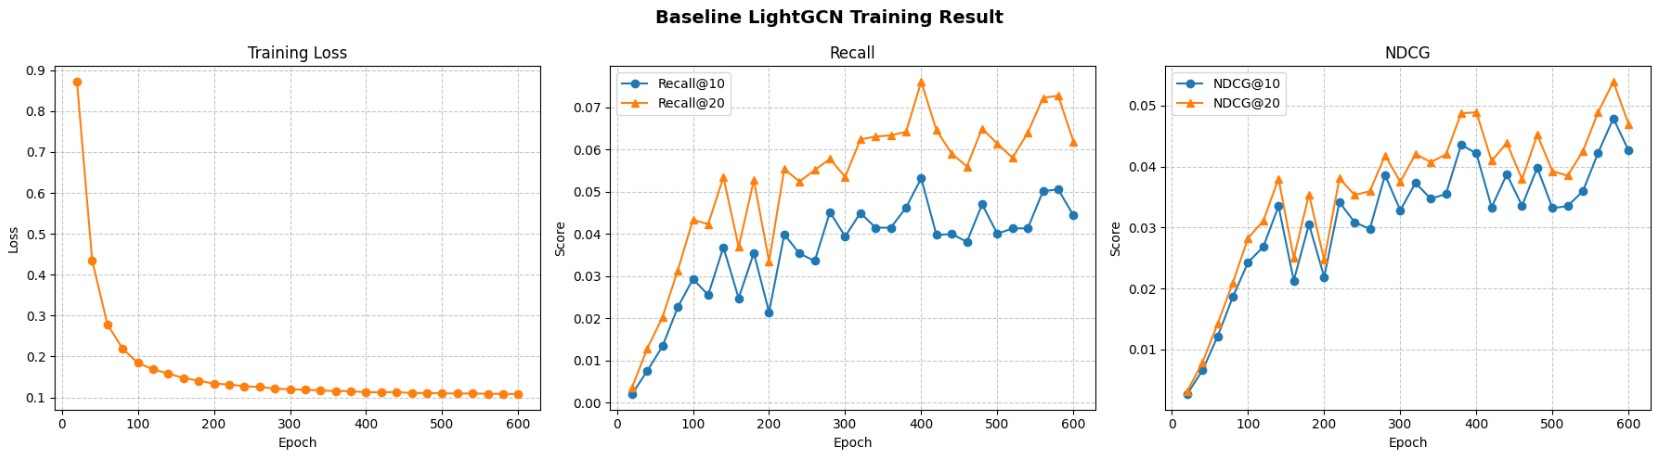
\includegraphics[width=\textwidth]{images/4image60.jpg}
\caption{กราฟผลการฝึกสอนของโมเดล Baseline LightGCN (Loss, Recall, NDCG)}
\label{fig:ch4_60}
\end{figure}

จากตารางที่ \ref{tab:ch4_38} โมเดล LightGCN ให้ค่า Loss สุดท้ายต่ำกว่าโมเดล MF เล็กน้อย 0.1082 เทียบกับ 0.1079 ของ MF ซึ่งใกล้เคียงกัน แต่ในแง่ความสามารถจัดอันดับกลับให้ผล NDCG@20 สูงสุดที่ Epoch 400 (0.0489) ก่อนจะแกว่งตัวลงในช่วงท้าย แสดงให้เห็นว่าการเพิ่ม Graph Convolution เพียงอย่างเดียวโดยไม่ผสานพฤติกรรมเสริมยังไม่สามารถให้ผลลัพธ์ที่เสถียรกว่าโมเดล MF ได้อย่างชัดเจน กราฟผลการฝึกสอนของโมเดล Baseline LightGCN แสดงในภาพที่ \ref{fig:ch4_60}

\subsubsection{ผลการทดสอบโมเดล MBRS (MB-CGCN สัดส่วนคงที่ Cart 10\% : Rent 90\%)}

โมเดล MBRS คือโมเดลที่นำเสนอในโครงงานนี้ ใช้สถาปัตยกรรม MB-CGCN แบบ Cascading พร้อมกำหนดสัดส่วนน้ำหนักคงที่ที่ Cart 10\% และ Rent 90\% ตามที่อธิบายไว้ในหัวข้อการออกแบบสถาปัตยกรรม ผลลัพธ์การฝึกสอนแสดงดังตารางที่ \ref{tab:ch4_39}

\begin{table}[H]
\centering
\caption{ประสิทธิภาพของโมเดล MBRS (Cart 10\% : Rent 90\%) ณ ช่วงเวลาต่างๆ}
\label{tab:ch4_39}
\small
\begin{tabular}{|c|c|c|c|c|c|}
\hline
\textbf{Epoch} & \textbf{Loss} & \textbf{Recall@10} & \textbf{NDCG@10} & \textbf{Recall@20} & \textbf{NDCG@20} \\ \hline
100 & 0.2059 & 0.0267 & 0.0229 & 0.0445 & 0.0284 \\ \hline
200 & 0.1545 & 0.0359 & 0.0297 & 0.0505 & 0.0340 \\ \hline
300 & 0.1386 & 0.0477 & 0.0393 & 0.0682 & 0.0456 \\ \hline
420 (Peak) & 0.1295 & 0.0574 & 0.0453 & 0.0799 & 0.0516 \\ \hline
500 & 0.1263 & 0.0411 & 0.0391 & 0.0666 & 0.0468 \\ \hline
600 & 0.1241 & 0.0478 & 0.0388 & 0.0708 & 0.0455 \\ \hline
\end{tabular}
\end{table}

\begin{figure}[H]
\centering
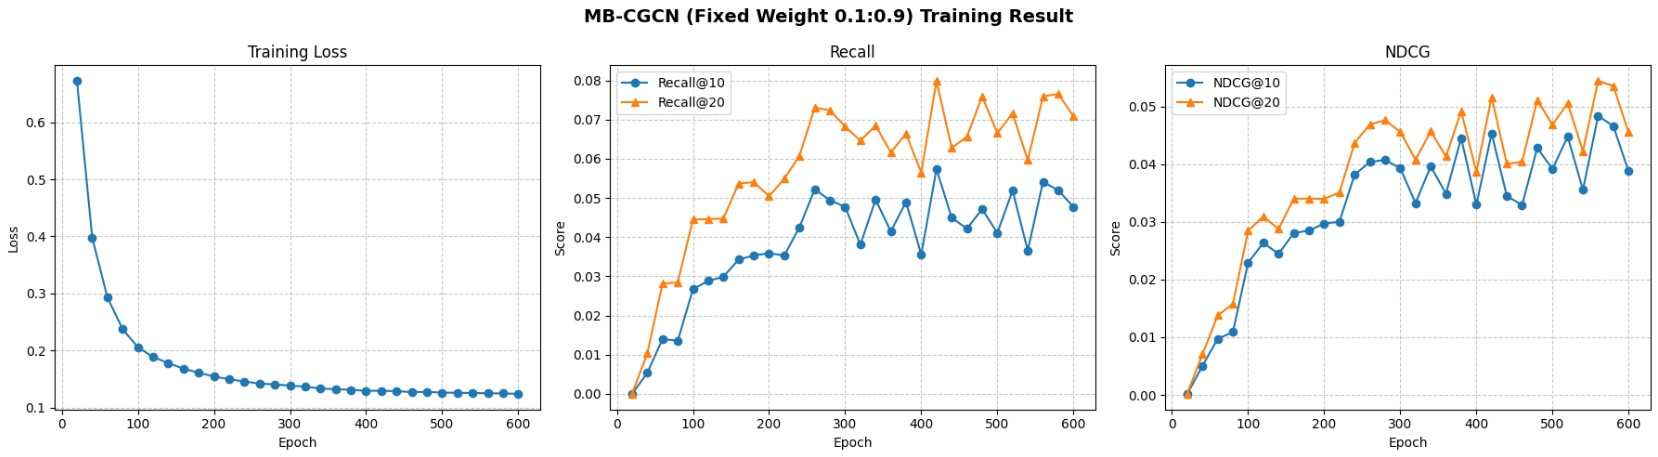
\includegraphics[width=\textwidth]{images/4image61.jpg}
\caption{กราฟผลการฝึกสอนของโมเดล MBRS สัดส่วนคงที่ 10:90 (Loss, Recall, NDCG)}
\label{fig:ch4_61}
\end{figure}

จากตารางที่ \ref{tab:ch4_39} โมเดล MBRS ทำจุดสูงสุด ที่ Epoch ประมาณ 420 โดยได้ค่า Recall@20 สูงถึง 7.99\% และ NDCG@20 อยู่ที่ 5.16\% ซึ่งสูงกว่าจุดสูงสุดของโมเดลฐานทั้งสองตัวในทุกช่วงที่วัดได้ สะท้อนว่าการนำสัญญาณจากพฤติกรรมการกดเข้าตะกร้า มาเป็นข้อมูลเสริมแบบ Cascading ก่อนจะเรียนรู้พฤติกรรมเป้าหมาย ช่วยให้โมเดลจับรูปแบบความสนใจของผู้ใช้ได้ดีขึ้นเมื่อเทียบกับการใช้ข้อมูลพฤติกรรมเดียว กราฟผลการฝึกสอนแสดงให้เห็นว่าค่า Loss ลดลงอย่างราบเรียบจาก 0.6725 (Epoch 20) เหลือ 0.1241 (Epoch 600) และค่า Recall@20 พัฒนาขึ้นอย่างต่อเนื่องตลอดการฝึกสอน กราฟผลการฝึกสอนของโมเดล MBRS แสดงในภาพที่ \ref{fig:ch4_61}

\subsubsection{การทดลองเปรียบเทียบ: สัดส่วนน้ำหนักแบบเรียนรู้เอง (Ablation Study)}

เพื่อยืนยันการเลือกใช้สัดส่วนน้ำหนักคงที่ Cart 10\% : Rent 90\% ได้ทำการทดลองเพิ่มเติมโดยปรับให้พารามิเตอร์น้ำหนัก $w_{cart}$ และ $w_{rent}$ เป็นค่าที่โมเดลเรียนรู้ได้เอง แทนการกำหนดค่าคงที่ ผลลัพธ์แสดงดังตารางที่ \ref{tab:ch4_40}

\begin{table}[H]
\centering
\caption{ประสิทธิภาพของโมเดล MB-CGCN แบบน้ำหนักเรียนรู้เอง ณ ช่วงเวลาต่างๆ}
\label{tab:ch4_40}
\footnotesize
\begin{tabular}{|c|c|c|c|c|c|c|}
\hline
\textbf{Epoch} & \textbf{Loss} & \textbf{Cart:Rent} & \textbf{Recall@10} & \textbf{NDCG@10} & \textbf{Recall@20} & \textbf{NDCG@20} \\ \hline
100 & 0.1839 & 0.478 : 0.522 & 0.0214 & 0.0179 & 0.0367 & 0.0221 \\ \hline
200 & 0.1400 & 0.483 : 0.517 & 0.0290 & 0.0241 & 0.0478 & 0.0296 \\ \hline
300 & 0.1266 & 0.486 : 0.514 & 0.0455 & 0.0345 & 0.0635 & 0.0401 \\ \hline
400 & 0.1202 & 0.488 : 0.512 & 0.0436 & 0.0372 & 0.0665 & 0.0434 \\ \hline
500 & 0.1167 & 0.489 : 0.511 & 0.0492 & 0.0403 & 0.0742 & 0.0477 \\ \hline
600 & 0.1161 & 0.490 : 0.510 & 0.0522 & 0.0420 & 0.0749 & 0.0494 \\ \hline
\end{tabular}
\end{table}

\begin{figure}[H]
\centering
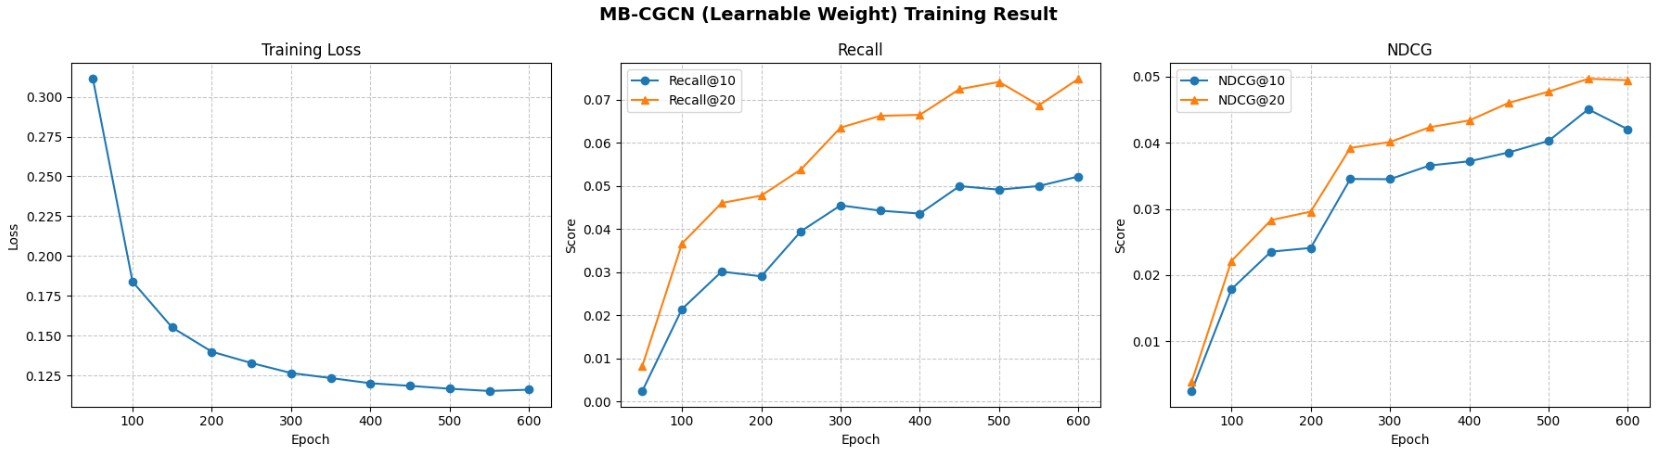
\includegraphics[width=\textwidth]{images/4image62.jpg}
\caption{กราฟผลการฝึกสอนของโมเดล MB-CGCN แบบน้ำหนักเรียนรู้เอง (Loss, Recall, NDCG)}
\label{fig:ch4_62}
\end{figure}

จากตารางที่ \ref{tab:ch4_40} จะเห็นว่าเมื่อปล่อยให้โมเดลปรับน้ำหนักเอง ค่า $w_{cart}$ และ $w_{rent}$ จะลู่เข้าใกล้สัดส่วนที่เกือบเท่ากัน ประมาณ 0.49 : 0.51 ตลอดการฝึกสอน แทนที่จะให้น้ำหนักกับพฤติกรรมเป้าหมาย มากเป็นพิเศษ ซึ่งสอดคล้องกับกราฟผลการฝึกสอนที่แสดงให้เห็นว่าสัดส่วนน้ำหนัก Cart:Rent ค่อยๆ เปลี่ยนจาก 0.478 : 0.522 (Epoch 100) เป็น 0.490 : 0.510 (Epoch 600) อย่างค่อยเป็นค่อยไป ซึ่งเมื่อเทียบค่าสูงสุด ที่ทำได้ตลอดการฝึกสอนกับโมเดล MBRS สัดส่วนคงที่ในตารางที่ \ref{tab:ch4_39} พบว่ารุ่นสัดส่วนคงที่ 10:90 สามารถทำค่า NDCG@20 สูงสุดได้มากกว่า 5.16\% ที่ Epoch 420 เทียบกับ 4.94\% ที่ Epoch 600 ของรุ่นน้ำหนักเรียนรู้เอง จึงเป็นเหตุผลสนับสนุนการเลือกใช้สัดส่วนคงที่ Cart 10\% : Rent 90\% เป็นค่าสุดท้ายของโมเดล MBRS ที่นำไปใช้งานจริงในระบบ ทั้งนี้เนื่องจากค่าที่วัดได้ในแต่ละ Epoch มาจากการสุ่มผู้ใช้ทดสอบเพียง 1,000 คน ผลต่างระหว่างสองแนวทางจึงควรพิจารณาร่วมกับแนวโน้มโดยรวมมากกว่าตัวเลข ณ จุดใดจุดหนึ่งเพียงจุดเดียว กราฟผลการฝึกสอนของโมเดล MB-CGCN แบบน้ำหนักเรียนรู้เองแสดงในภาพที่ \ref{fig:ch4_62}

\subsubsection{ผลเปรียบเทียบประสิทธิภาพสุดท้ายระหว่างโมเดลทั้งหมด (Final Performance Comparison)}

เพื่อสรุปภาพรวม ได้นำผลลัพธ์ ณ Epoch สุดท้าย ของทั้ง 3 โมเดลหลัก ได้แก่ MBRS (MB-CGCN สัดส่วนคงที่ 10:90), Baseline MF และ Baseline LightGCN มาเปรียบเทียบกันโดยตรงใน 4 ตัวชี้วัด ดังภาพที่ \ref{fig:ch4_63} และตารางที่ \ref{tab:ch4_41}

\begin{figure}[H]
\centering
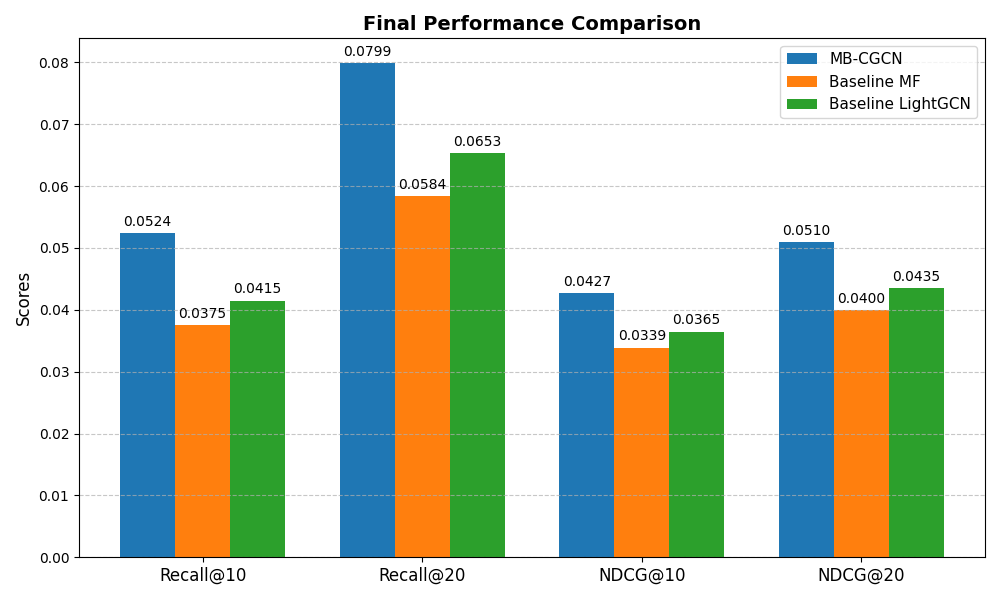
\includegraphics[width=0.85\textwidth]{images/4image63.png}
\caption{กราฟแท่งเปรียบเทียบผลลัพธ์สุดท้าย (Epoch 600) ของทั้ง 3 โมเดล}
\label{fig:ch4_63}
\end{figure}

กราฟแท่งในภาพที่ \ref{fig:ch4_63} แสดงผลลัพธ์เปรียบเทียบ 4 ตัวชี้วัด ได้แก้ Recall@10, Recall@20, NDCG@10, NDCG@20 ของโมเดลทั้ง 3 ตัว ณ Epoch สุดท้าย ซึ่งจะเห็นได้ว่าโมเดล MBRS ทำคะแนนได้สูงสุดในทุกตัวชี้วัดอย่างชัดเจน ขณะที่ Baseline MF และ Baseline LightGCN ทำคะแนนได้ต่ำกว่าในทุกมิติ

\begin{table}[H]
\centering
\caption{เปรียบเทียบประสิทธิภาพสุดท้าย (Epoch 600) ระหว่างโมเดลทั้งหมด}
\label{tab:ch4_41}
\small
\begin{tabular}{|p{4cm}|c|c|c|c|}
\hline
\textbf{โมเดล} & \textbf{Recall@10} & \textbf{Recall@20} & \textbf{NDCG@10} & \textbf{NDCG@20} \\ \hline
MBRS (MB-CGCN 10:90) & \textbf{0.0524} & \textbf{0.0799} & \textbf{0.0427} & \textbf{0.0510} \\ \hline
Baseline MF & 0.0375 & 0.0584 & 0.0339 & 0.0400 \\ \hline
Baseline LightGCN & 0.0415 & 0.0653 & 0.0365 & 0.0435 \\ \hline
\end{tabular}
\end{table}

\begin{figure}[H]
\centering
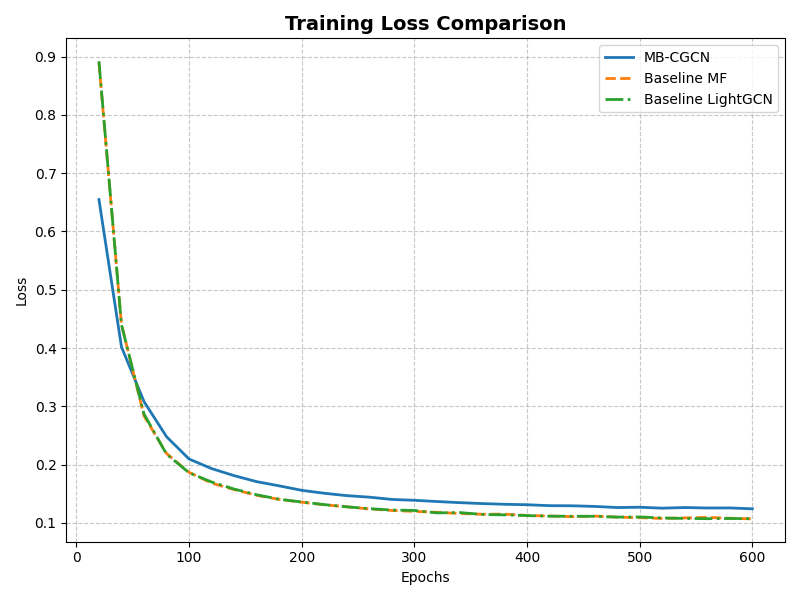
\includegraphics[width=\textwidth]{images/4image64.png}
\caption{กราฟเปรียบเทียบ Training Loss ระหว่างทั้ง 3 โมเดลตลอดการฝึกสอน}
\label{fig:ch4_64}
\end{figure}

กราฟเปรียบเทียบ Training Loss ในภาพที่ \ref{fig:ch4_64} แสดงแนวโน้มค่า Loss ของโมเดลทั้ง 3 ตัวตลอด 600 Epoch จะเห็นได้ว่าทั้ง 3 โมเดลมีแนวโน้ม Loss ลดลงในทิศทางเดียวกัน โดย MBRS มีค่า Loss สูงกว่า MF และ LightGCN  เล็กน้อยในช่วงแรก เนื่องจากต้องเรียนรู้จากข้อมูลพฤติกรรมหลายชั้น แต่ในช่วงท้าย Loss ลดลงจนใกล้เคียงกัน แสดงว่าโมเดล MBRS เรียนรู้ได้สำเร็จแม้จะมีโครงสร้างที่ซับซ้อนกว่า

\begin{figure}[H]
\centering
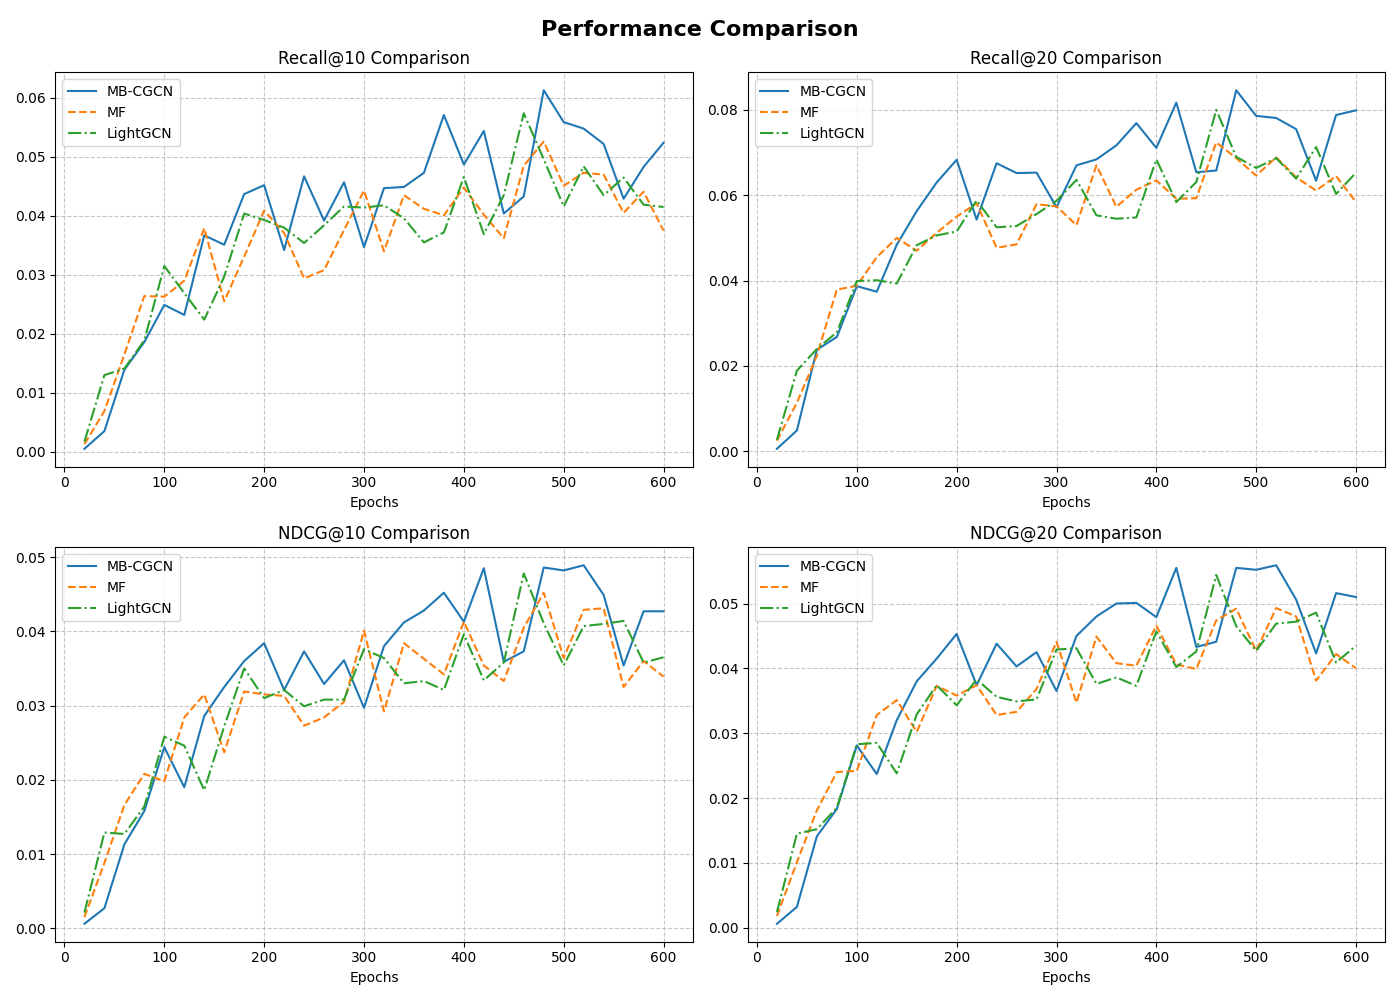
\includegraphics[width=\textwidth]{images/4image65.png}
\caption{กราฟเปรียบเทียบ Recall@10, Recall@20, NDCG@10 และ NDCG@20 ของทั้ง 3 โมเดลตลอดการฝึกสอน}
\label{fig:ch4_65}
\end{figure}

กราฟเปรียบเทียบเมตริกในภาพที่ \ref{fig:ch4_65} แสดงแนวโน้ม Recall@10, Recall@20, NDCG@10 และ NDCG@20 ของโมเดลทั้ง 3 ตัวตลอดการฝึกสอนในรูปแบบ 2$\times$2 กราฟย่อย จะเห็นได้ว่าในทุกตัวชี้วัด MBRS มีแนวโน้มสูงขึ้นอย่างต่อเนื่องและมักอยู่เหนือ MF และ LightGCN ในช่วง Epoch ที่ 200 เป็นต้นไป โดยเฉพาะใน Recall@20 และ NDCG@20 ซึ่ง MBRS เริ่มทิ้งห่างจากโมเดลฐานอย่างชัดเจนในช่วง Epoch 300--600 ยืนยันว่าการผสานพฤติกรรมแบบ Cascading ช่วยเพิ่มความสามารถในการจัดอันดับคำแนะนำอย่างมีนัยสำคัญ

จากตารางที่ \ref{tab:ch4_41} พบว่าโมเดล MBRS ที่นำเสนอในโครงงานนี้ทำคะแนนสูงสุดในทุกตัวชี้วัดเมื่อเทียบกับโมเดลฐานทั้งสองตัว ณ Epoch สุดท้าย โดยให้ค่า Recall@20 สูงกว่า Baseline MF ราวร้อยละ 37 และสูงกว่า Baseline LightGCN ราวร้อยละ 22 ยืนยันว่าการออกแบบสถาปัตยกรรมแบบ Cascading ที่ผสานพฤติกรรมตะกร้า เข้ากับพฤติกรรมการเช่า ให้ผลลัพธ์ในการแนะนำที่ดีกว่าการใช้ข้อมูลพฤติกรรมเดียว (Single-Behavior) ไม่ว่าจะเป็นแบบไม่มีกราฟ (MF) หรือมีกราฟแต่ไม่ผสานพฤติกรรม (LightGCN) ทั้งนี้ผลต่างระหว่างโมเดลยังอยู่ในระดับปานกลาง ซึ่งส่วนหนึ่งเป็นผลจากความหนาแน่นของข้อมูลพฤติกรรม Cart ที่มีจำนวนน้อยกว่าพฤติกรรม Rent ค่อนข้างมาก และยังไม่ได้รวมพฤติกรรมการคลิกอ่านเนื้อหา เข้ามาด้วยตามที่อธิบายไว้ในขอบเขตของโครงงาน

\subsubsection{ผลการทดสอบโมเดลเวอร์ชัน 2 (MB-CGCN v2) แบบสามพฤติกรรม}

หลังจากพัฒนาและใช้งานโมเดลเวอร์ชันแรก (v1) ที่ใช้พฤติกรรมสองลำดับ Cart $\to$ Rent เป็นโมเดลหลักในระบบเว็บแอปพลิเคชันแล้ว ทีมผู้พัฒนาได้ขยายโมเดลเป็นเวอร์ชันที่สอง (v2) ซึ่งเพิ่มพฤติกรรม Click เข้ามาเป็นพฤติกรรมเสริมลำดับแรก ทำให้สายโซ่พฤติกรรมเป็น Click $\to$ Cart $\to$ Rent และเปลี่ยนน้ำหนักรวมพฤติกรรมจากค่าคงที่เป็นน้ำหนักที่ปรับได้ระหว่างการฝึกสอน การเปลี่ยนแปลงนี้มีจุดประสงค์เพื่อให้โมเดลเรียนรู้สัญญาณความสนใจของผู้ใช้ได้ตั้งแต่ขั้นตอนการดูรายละเอียดหนังสือ ก่อนจะมีการหยิบลงตะกร้าหรือทำการเช่าจริง และให้โมเดลสามารถเรียนรู้ได้เองว่าพฤติกรรมใดควรมีอิทธิพลต่อผลการทำนายมากหรือน้อยกว่ากัน แทนการกำหนดสัดส่วนคงที่โดยผู้พัฒนา

ทั้งนี้เนื่องจากเว็บแอปพลิเคชันเพิ่งพัฒนาเสร็จและยังไม่มีผู้ใช้งานจริงจำนวนมากพอสำหรับการฝึกสอนโมเดล v2 ผู้พัฒนาจึงสร้างข้อมูลพฤติกรรมจำลอง ของผู้ใช้ 1,000 คนกับหนังสือการ์ตูน 100 เรื่อง โดยมีพฤติกรรมครบทั้งสามประเภทตามห่วงโซ่ Click $\to$ Cart $\to$ Rent เพื่อทดสอบกลไกการฝึกสอนและประเมินประสิทธิภาพของโมเดล v2 ได้ล่วงหน้า ข้อมูลจำลองนี้ถูกสร้างให้มีลักษณะสอดคล้องกับโครงสร้างข้อมูลจริงของระบบ และถูกแบ่งออกเป็นชุดฝึกสอนและชุดทดสอบในสัดส่วน 80:20 เช่นเดียวกับข้อมูลของโมเดล v1

โมเดล v2 ถูกฝึกสอนบนข้อมูลจำลองนี้ภายใต้พารามิเตอร์ชุดเดียวกับโมเดล v1 แต่มีความแตกต่างในรายละเอียดดังนี้ จำนวนเลเยอร์ GCN ของพฤติกรรมเช่า เพิ่มเป็น 2 ชั้น มีเลเยอร์เพิ่มเติมสำหรับพฤติกรรม Click และน้ำหนักรวมพฤติกรรม เปลี่ยนจากค่าคงที่เป็นค่าที่ปรับได้ระหว่างฝึกสอน เพื่อเปรียบเทียบประสิทธิภาพของโมเดล v2 กับโมเดลฐาน ผู้พัฒนาได้ฝึกสอนโมเดลฐานเพิ่มเติม 2 ตัวบนชุดข้อมูลจำลองชุดเดียวกัน ได้แก่ Baseline MF และ Baseline LightGCN นอกจากนี้ยังมีการเปรียบเทียบกับ Baseline Popularity ซึ่งเป็นโมเดลที่แนะนำหนังสือโดยอิงจากจำนวนครั้งที่ถูกเช่าโดยรวมมากที่สุด เพื่อเป็น Baseline พื้นฐานที่สุด ผลลัพธ์การฝึกสอนและการเปรียบเทียบแสดงดังตารางที่ \ref{tab:ch4_42} และภาพที่ \ref{fig:ch4_115}, \ref{fig:ch4_116} และ \ref{fig:ch4_117}

\begin{table}[H]
\centering
\caption{ประสิทธิภาพของโมเดล MB-CGCN v2 และโมเดลฐาน ณ ช่วงเวลาต่างๆ}
\label{tab:ch4_42}
\small
\begin{tabular}{|c|c|c|c|c|c|c|}
\hline
\textbf{โมเดล} & \textbf{Epoch} & \textbf{Loss} & \textbf{Recall@10} & \textbf{NDCG@10} & \textbf{Recall@20} & \textbf{NDCG@20} \\ \hline
\multirow{7}{*}{MB-CGCN v2}
& 1 & 0.6867 & 0.1399 & 0.0865 & 0.2744 & 0.1277 \\ \cline{2-7}
& 100 & 0.6931 & 0.1939 & 0.1223 & 0.3220 & 0.1621 \\ \cline{2-7}
& 200 & 0.6931 & 0.2400 & 0.1427 & 0.3642 & 0.1820 \\ \cline{2-7}
& 300 & 0.6931 & 0.2273 & 0.1360 & 0.3833 & 0.1832 \\ \cline{2-7}
& 400 & 0.6931 & 0.2213 & 0.1343 & 0.3719 & 0.1816 \\ \cline{2-7}
& 500 & 0.6931 & 0.2133 & 0.1325 & 0.3632 & 0.1785 \\ \cline{2-7}
& 600 & 0.6931 & \textbf{0.2158} & \textbf{0.1318} & \textbf{0.3522} & \textbf{0.1742} \\ \hline
\multirow{7}{*}{MF}
& 1 & 0.8195 & 0.1046 & 0.0591 & 0.2253 & 0.0957 \\ \cline{2-7}
& 100 & 0.4609 & 0.1017 & 0.0573 & 0.1991 & 0.0878 \\ \cline{2-7}
& 200 & 0.5280 & 0.1187 & 0.0696 & 0.2275 & 0.1028 \\ \cline{2-7}
& 300 & 0.5563 & 0.1291 & 0.0746 & 0.2368 & 0.1073 \\ \cline{2-7}
& 400 & 0.5685 & 0.1474 & 0.0854 & 0.2497 & 0.1175 \\ \cline{2-7}
& 500 & 0.5639 & 0.1360 & 0.0854 & 0.2665 & 0.1256 \\ \cline{2-7}
& 600 & 0.5604 & 0.1614 & 0.0956 & 0.2705 & 0.1303 \\ \hline
\multirow{7}{*}{LightGCN}
& 1 & 0.6042 & 0.1028 & 0.0562 & 0.2219 & 0.0929 \\ \cline{2-7}
& 100 & 0.6664 & 0.1090 & 0.0641 & 0.2108 & 0.0960 \\ \cline{2-7}
& 200 & 0.6890 & 0.1113 & 0.0667 & 0.2153 & 0.0988 \\ \cline{2-7}
& 300 & 0.6928 & 0.1099 & 0.0686 & 0.2161 & 0.1017 \\ \cline{2-7}
& 400 & 0.6931 & 0.1113 & 0.0745 & 0.2353 & 0.1118 \\ \cline{2-7}
& 500 & 0.6931 & 0.1217 & 0.0747 & 0.2381 & 0.1095 \\ \cline{2-7}
& 600 & 0.6931 & 0.1224 & 0.0748 & 0.2507 & 0.1134 \\ \hline
\end{tabular}
\end{table}

\begin{figure}[H]
\centering
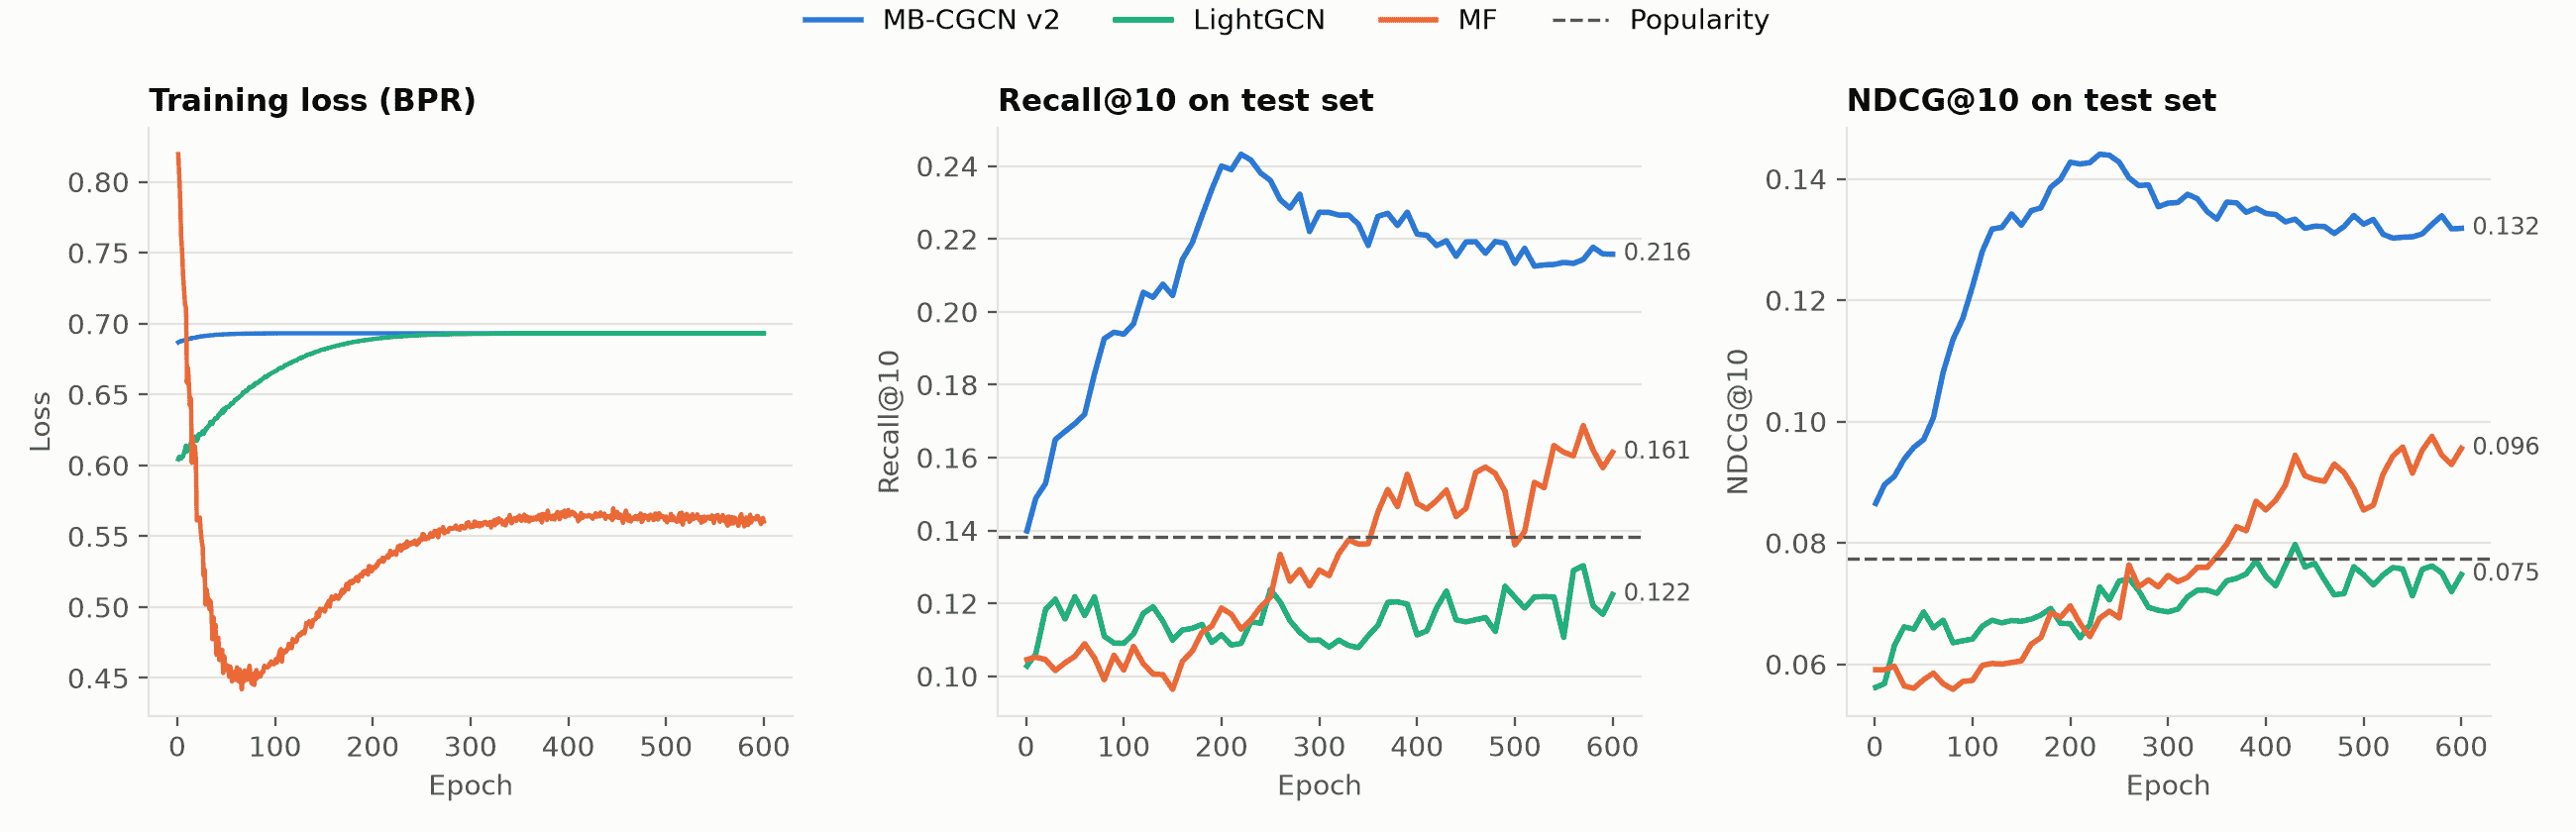
\includegraphics[width=0.9\textwidth]{images/fig_ch4_v2_learning_curve.png}
\caption{กราฟผลการฝึกสอนของโมเดล MB-CGCN v2 (Loss, Recall@10, NDCG@10)}
\label{fig:ch4_115}
\end{figure}

จากตารางที่ \ref{tab:ch4_42} และภาพที่ \ref{fig:ch4_115} พบว่าโมเดล MB-CGCN v2 มีค่า Loss ค่อนข้างคงที่ตลอดการฝึกสอน เริ่มต้นที่ 0.6867 และลู่เข้าสู่ 0.6931 ตั้งแต่ Epoch 100 แตกต่างจาก MF และ LightGCN ที่มีแนวโน้ม Loss เพิ่มขึ้น MF เริ่มต้นที่ 0.8195 แล้วลดลงมาอยู่ที่ 0.5604 ณ Epoch 600 ขณะที่ LightGCN เพิ่มขึ้นจาก 0.6042 มาอยู่ที่ 0.6931 พฤติกรรมนี้สะท้อนธรรมชาติของฟังก์ชันสูญเสีย BPR Loss ที่วัดจากผลต่างคะแนนระหว่างคู่ Positive และ Negative ซึ่งไม่จำเป็นต้องมีความสัมพันธ์เชิงเดียวกับตัวชี้วัดอันดับเสมอไป ในแง่ของความสามารถจัดอันดับ โมเดล v2 เริ่มต้นที่ Recall@10 = 13.99\% และพัฒนาขึ้นอย่างต่อเนื่องจนถึงจุดสูงสุดที่ Epoch 200 ก่อนจะแกว่งตัวลดลงเล็กน้อยในช่วง Epoch 300 - 600 และจบที่ Epoch 600 ด้วย Recall@10 = 21.58\% และ NDCG@10 = 13.18\% ซึ่งสูงกว่า MF และ LightGCN อย่างชัดเจน ส่วนค่า Recall@20 และ NDCG@20 ของโมเดล v2 ณ Epoch 600 อยู่ที่ 35.22\% และ 17.42\% ตามลำดับ ซึ่งสูงกว่าโมเดลฐานทั้งสองตัวเช่นกัน

\begin{figure}[H]
\centering
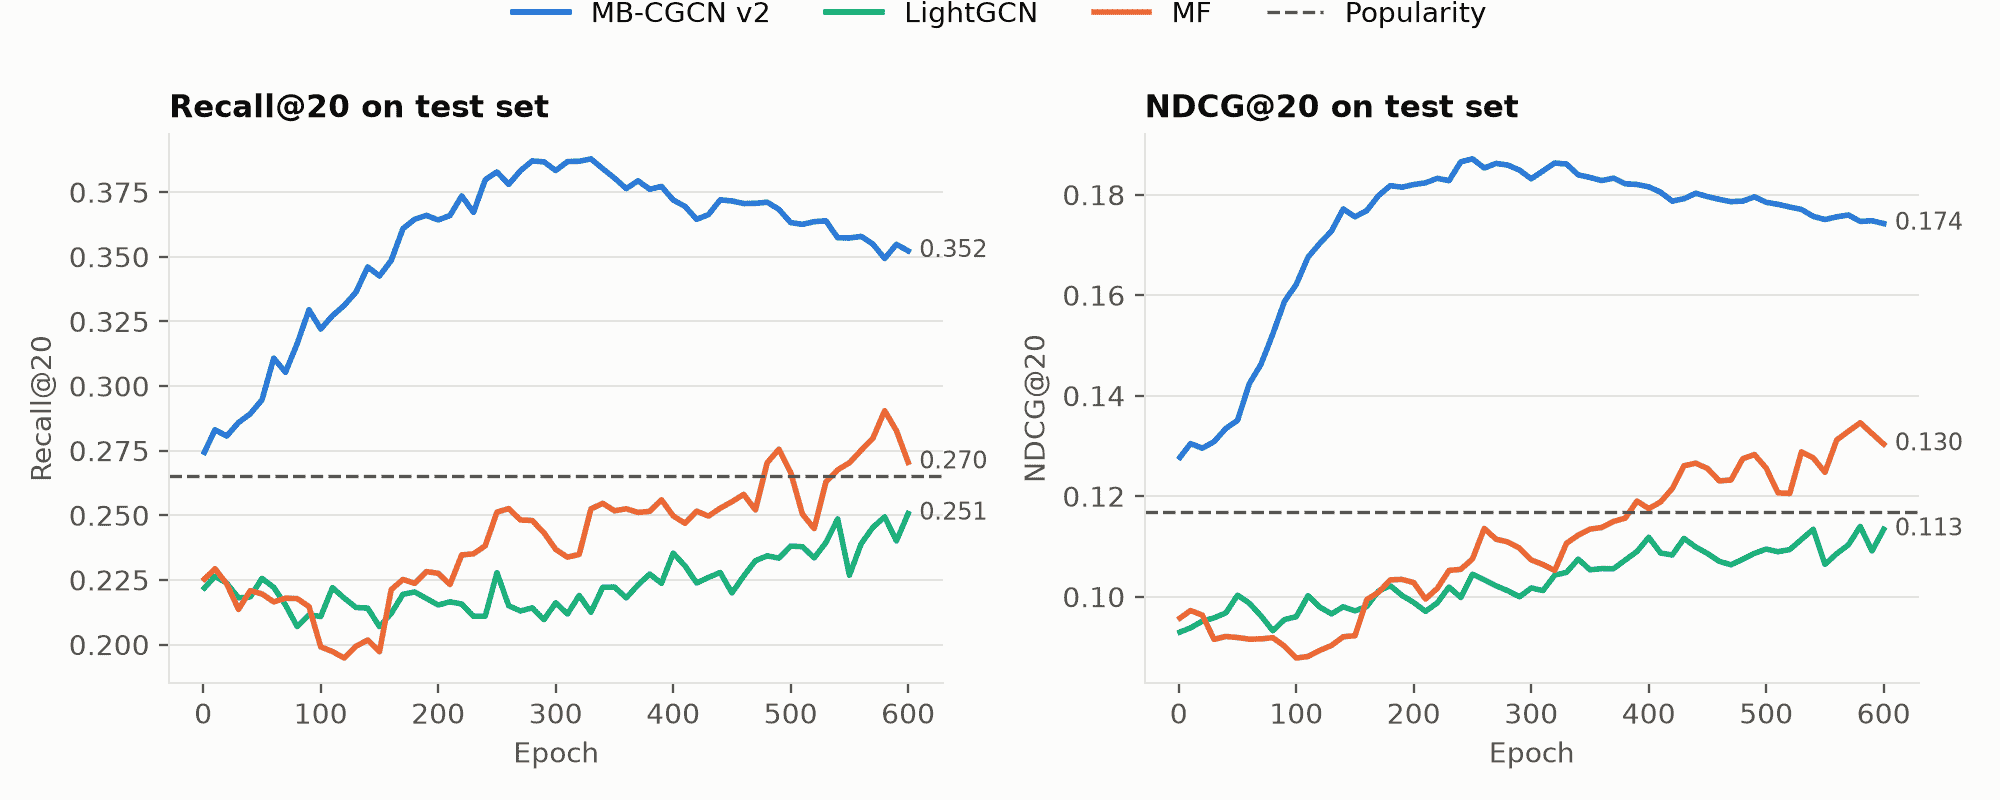
\includegraphics[width=0.9\textwidth]{images/fig_ch4_v2_learning_curve_at20.png}
\caption{กราฟผลการฝึกสอนของโมเดล MB-CGCN v2 (Recall@20, NDCG@20)}
\label{fig:ch4_116}
\end{figure}

ภาพที่ \ref{fig:ch4_116} แสดงแนวโน้ม Recall@20 และ NDCG@20 ของโมเดล v2 เปรียบเทียบกับโมเดลฐานตลอดการฝึกสอน จะเห็นได้ว่าเส้นของโมเดล v2 อยู่เหนือเส้นของ MF และ LightGCN ตลอดเกือบทั้งหมด โดยเฉพาะในช่วง Epoch 150 - 350 ที่โมเดล v2 ทำจุดสูงสุด Recall@20 ถึง 38.70\% ก่อนจะคงที่อยู่ในระดับ 35 - 37\% ในช่วงท้าย ขณะที่ MF และ LightGCN ทำคะแนนได้เพียง 27\% และ 25\% ตามลำดับ แสดงให้เห็นว่าการเพิ่มพฤติกรรม Click เข้ามาช่วยให้โมเดลจับรูปแบบความสนใจของผู้ใช้ได้ดีขึ้น แม้ว่าข้อมูลจะเป็นข้อมูลจำลองก็ตาม

นอกจากนี้ น้ำหนักพฤติกรรมที่ปรับได้ (Adaptive Behavior Weights) ของโมเดล v2 เริ่มต้นที่สัดส่วน Click : Cart : Rent = 0.0629 : 0.1710 : 0.7662 และค่อยๆ เปลี่ยนแปลงไปเป็น 0.0730 : 0.1736 : 0.7534 ณ Epoch 600 สะท้อนว่าโมเดลให้น้ำหนักกับพฤติกรรม Click เพิ่มขึ้นเล็กน้อยตลอดการฝึกสอน (จาก 6.29\% เป็น 7.30\%) ขณะที่น้ำหนักของ Rent ลดลงเล็กน้อย (จาก 76.62\% เป็น 75.34\%) และน้ำหนักของ Cart คงที่ประมาณ 17\% แสดงว่าโมเดลเรียนรู้ได้เองว่าพฤติกรรม Rent ยังคงเป็นสัญญาณหลัก แต่พฤติกรรม Click และ Cart ก็มีอิทธิพลเสริมที่สำคัญในการทำนายความสนใจของผู้ใช้

\begin{figure}[H]
\centering
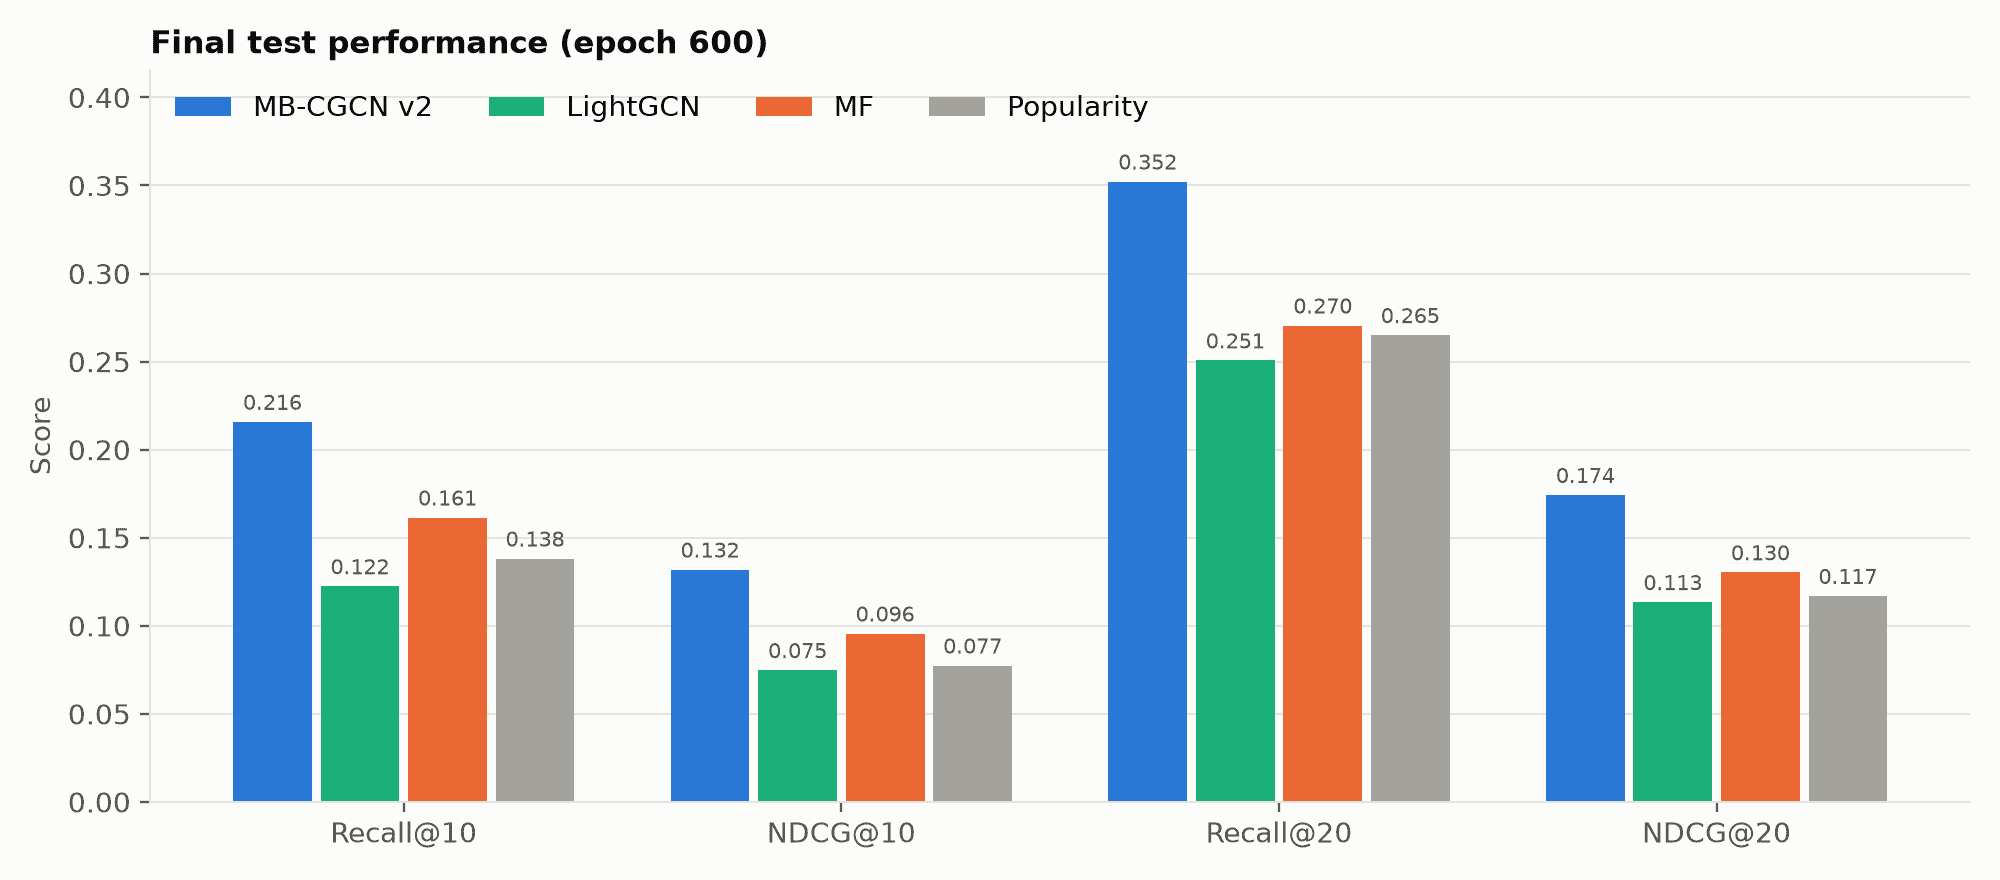
\includegraphics[width=0.85\textwidth]{images/fig_ch4_v2_vs_popularity_bar.png}
\caption{กราฟแท่งเปรียบเทียบผลลัพธ์สุดท้าย ของโมเดล v2 กับโมเดลฐานทั้งหมด}
\label{fig:ch4_117}
\end{figure}

ภาพที่ \ref{fig:ch4_117} แสดงกราฟแท่งเปรียบเทียบประสิทธิภาพสุดท้ายของโมเดล MB-CGCN v2 กับโมเดลฐานทั้งหมด ได้แก่ MF, LightGCN และ Popularity ในตัวชี้วัดทั้งสี่ตัว จะเห็นได้ชัดเจนว่าโมเดล v2 ทำคะแนนได้สูงสุดในทุกตัวชี้วัด โดยเฉพาะ Recall@10 ที่สูงกว่า Popularity (13.81\%) ถึงร้อยละ 56 และสูงกว่า LightGCN ถึงร้อยละ 76 ยืนยันว่าการออกแบบโมเดลแบบหลายพฤติกรรม ร่วมกับกลไกน้ำหนักที่ปรับได้ ให้ผลลัพธ์ที่ดีกว่าโมเดลพฤติกรรมเดียวและโมเดล Popularity อย่างมีนัยสำคัญ

สรุปได้ว่าโมเดล MB-CGCN v2 แม้จะฝึกสอนบนข้อมูลจำลองเพียง 1,000 ผู้ใช้และ 100 หนังสือ แต่ก็แสดงให้เห็นความสามารถในการเรียนรู้รูปแบบพฤติกรรมแบบ Cascading (Click $\to$ Cart $\to$ Rent) ได้อย่างมีประสิทธิภาพ และให้ผลการจัดอันดับที่ดีกว่าโมเดลฐานทั้งหมดอย่างชัดเจน โดยมีค่า Recall@10 และ NDCG@10 ที่ Epoch สุดท้ายอยู่ที่ 21.58\% และ 13.18\% ตามลำดับ ซึ่งเป็นไปตามสมมติฐานที่ว่าการเพิ่มสัญญาณพฤติกรรมเสริม จะช่วยเพิ่มความแม่นยำของการทำนายพฤติกรรมเป้าหมายได้ เมื่อระบบมีผู้ใช้จริงมากขึ้นและข้อมูลพฤติกรรมสะสมเพียงพอ ผู้ดูแลระบบจะสามารถฝึกโมเดล v2 ใหม่จากข้อมูลจริงผ่านหน้าแดชบอร์ดได้ และผลลัพธ์ที่ได้จากข้อมูลจริงจะสะท้อนรูปแบบความสนใจของผู้ใช้งานจริงอย่างแท้จริง ซึ่งคาดว่าจะให้ประสิทธิภาพที่ดีกว่าการฝึกจากข้อมูลจำลองอีกด้วย